%%%
% Compile com latexmk -xelatex -synctex=1 ifes8-tcc.tex para usar Arial.
\documentclass[arial,centeredequations,english,brazilian,oneside,section=TITLE]{ifes8}

\usepackage{lastpage}           % Usado pelo exemplo de ficha catalográfica
\usepackage[alf,abnt-full-initials=yes]{abntex2cite} % Esta opção é exigida pelas normas do ifes.

% Ajuste ABNT NBR 10520:2023 (Citações autor-data em caixa mista)
\makeatletter
\renewcommand{\citeauthor}{\citeauthoronline}
\makeatother

\usepackage{microtype}          % para melhorias de justificação
\setlength{\emergencystretch}{2em}
\usepackage{morefloats}         % permite mais floats
\usepackage{blindtext}          % para gerar texto aleatório (dummy text)
\usepackage{tikz}
\usetikzlibrary[topaths]
\usepackage{mathtools}
\usepackage{xcolor}
\usepackage{algorithm}
\usepackage{algpseudocode}
\usepackage{textcomp}
\usepackage{eurosym}
\usepackage{listings}
%%% Define que todos os códigos fontes construídos com o ambiente
%%% `lstlisting' terão uma borda simples.
\definecolor{mygreen}{rgb}{0,0.6,0}
\definecolor{mygray}{rgb}{0.5,0.5,0.5}
\definecolor{mymauve}{rgb}{0.58,0,0.82}

\lstset{%
  backgroundcolor=\color{white},   % choose the background color
  basicstyle=\footnotesize,        % size of fonts used for the code
  breaklines=true,                 % automatic line breaking only at whitespace
  captionpos=b,                    % sets the caption-position to bottom
  commentstyle=\color{mygreen},    % comment style
  escapeinside={\%*}{*)},          % if you want to add LaTeX within your code
  keywordstyle=\color{blue},       % keyword style
  stringstyle=\color{mymauve}, 
  numbers=left,
  numberstyle=\scriptsize,
  stepnumber=1,    
  firstnumber=1,
  numberfirstline=true % string literal style,
  frame=single,
  literate=
  {á}{{\'a}}1 {é}{{\'e}}1 {í}{{\'i}}1 {ó}{{\'o}}1 {ú}{{\'u}}1
  {Á}{{\'A}}1 {É}{{\'E}}1 {Í}{{\'I}}1 {Ó}{{\'O}}1 {Ú}{{\'U}}1
  {à}{{\`a}}1 {è}{{\`e}}1 {ì}{{\`i}}1 {ò}{{\`o}}1 {ù}{{\`u}}1
  {À}{{\`A}}1 {È}{{\'E}}1 {Ì}{{\`I}}1 {Ò}{{\`O}}1 {Ù}{{\`U}}1
  {ä}{{\"a}}1 {ë}{{\"e}}1 {ï}{{\"i}}1 {ö}{{\"o}}1 {ü}{{\"u}}1
  {Ä}{{\"A}}1 {Ë}{{\"E}}1 {Ï}{{\"I}}1 {Ö}{{\"O}}1 {Ü}{{\"U}}1
  {â}{{\^a}}1 {ê}{{\^e}}1 {î}{{\^i}}1 {ô}{{\^o}}1 {û}{{\^u}}1
  {Â}{{\^A}}1 {Ê}{{\^E}}1 {Î}{{\^I}}1 {Ô}{{\^O}}1 {Û}{{\^U}}1
  {œ}{{\oe}}1 {Œ}{{\OE}}1 {æ}{{\ae}}1 {Æ}{{\AE}}1 {ß}{{\ss}}1
  {ű}{{\H{u}}}1 {Ű}{{\H{U}}}1 {ő}{{\H{o}}}1 {Ő}{{\H{O}}}1
  {ç}{{\c c}}1 {Ç}{{\c C}}1 {ø}{{\o}}1 {å}{{\r a}}1 {Å}{{\r A}}1
  {€}{{\EUR}}1 {£}{{\pounds}}1
}

\renewcommand{\lstlistingname}{Código Fonte}

%%% Local Variables:
%%% mode: latex
%%% TeX-master: "ifes8-tcc-ex"
%%% End:


%%% Definição da linguagem padrão do documento (pacote babel) para
%%% definir que certas porções do texto (como o resumo, por exemplo)
%%% estão em uma língua estrangeira, usar as macros
%%% \foreignlanguage{languageB}{Text in another language}
%%% ou
%%% \begin{otherlanguage}{languageB}
%%% ...
%%% \end{otherlanguage}
\selectlanguage{brazilian}

%%% Ajuste do alinhamento do caption de figuras, tabelas e quadros.
% \captionstyle{\raggedright}
% \normalcaption
% \normalcaptionwidth
% \captionwidth{\linewidth}


%%% Define que todos os códigos fontes construídos com o ambiente
%%% `lstlisting' terão uma borda simples.
\lstset{frame=single}

\titulo{Metodologia para Caracterização Viscoelástica e Dimensionamento de Enrijecedores à Flexão para Risers Flexíveis}

\autor{Alexandre Lima Simões\\Pedro Antônio Gomes Goronci}
\autorficha{Simões, Alexandre Lima; Goronci, Pedro Antônio Gomes}

\orientador{Prof. Dr. Vinicius Erler de Souza Ramos}

% \coorientadora{Prof.ª Dr.ª Fulana Detal Longname}

\instituicao{Instituto Federal do Espírito Santo}

\curso{Bacharelado em Engenharia Mecânica}

\data{2026}

\local{Vitória, ES}

\preambulo{Trabalho de Conclusão de Curso apresentado à Coordenadoria
  do Curso de Engenharia Mecânica do Instituto Federal do Espírito
  Santo, Campus Serra, como requisito parcial para a obtenção do
  título de Bacharel em Engenharia Mecânica.}

\tipotrabalho{Trabalho de Conclusão de Curso}



\begin{document}

%%% A macro \pretextual não precisa ser explicitamente chamada porque
%%% o abntex2 aciona essa macro no início do documento.
% \pretextual

\imprimircapa
\addtocounter{page}{-1}

\imprimirfolhaderosto*

\begin{fichacatalografica}
  \vspace*{\fill}
  % Posição vertical
  \begin{center}
    % Minipage Centralizado
    \fbox{
      \begin{minipage}[t]{12.5cm}
        \vspace*{3mm}
        \begin{minipage}[t]{2cm}
          X000x
        \end{minipage}
        \begin{minipage}[t]{10cm}
          \imprimirautorficha.\vspace{2mm}

          \hspace{0.5cm}\imprimirtitulo\ / \imprimirautor. ---
          \imprimirlocal, \imprimirdata.\\ 

          \hspace{0.5cm}\pageref{LastPage} p.:\ il. (algumas color.);
          30 cm.\\ 

          \hspace{0.5cm}\imprimirorientadorRotulo~\imprimirorientador.\\

          \hspace{0.5cm}\imprimirtipotrabalho\ ---
          \imprimirinstituicao, \imprimirdata\\

          \hspace{0.5cm}        
          1. Viscoelasticidade.
          2. Engenharia do petróleo.
          3. Equações diferenciais.
          4. Métodos numéricos.
          I. Vinicius Erler de Souza Ramos.
          II. Instituto Federal do Espírito Santo.
          III. Campus Vitória.
          IV. Título.
          
          \begin{flushright}
            CDU 00:000:000.0
          \end{flushright}
          \vspace*{1mm}
        \end{minipage}
      \end{minipage}
    }
    
    \vspace*{3mm}
    {\footnotesize Bibliotecário(a) responsável: Nome Completo -- CRB X/XXXX}
  \end{center}
\end{fichacatalografica}
\addtocounter{page}{-1}

%%% ====================================================================
%%% Exemplo de construção da folha de aprovação. Depois da
%%% apresentação do trabalho, quando a folha de apresentação real
%%% tiver sido assinada pela banca, a folha real deve ser digitalizada
%%% e o ambiente abaixo deve ser substituído por:
%%% \includepdf{folhadeaprovacao_final.pdf}
\begin{folhadeaprovacao}
  \begin{center}
    {\ABNTEXchapterfont\MakeTextUppercase{\imprimirautor}}\\
    \begin{center}
      \ABNTEXchapterfont\MakeTextUppercase{\imprimirtitulo}\\
    \end{center}
    \hspace{.45\textwidth}
    \begin{minipage}{.5\textwidth}
      {\footnotesize{\imprimirpreambulo}}\\
    \end{minipage}%
  \end{center}
  % \vspace{-1cm}%
  \begin{center}
    Aprovado em 11 de agosto de 2026.\\[15mm]
    \textbf{COMISSÃO EXAMINADORA}\\[5mm]
    \assinatura{\imprimirorientador \\
      Instituto Federal do Espírito Santo \\
      Orientador}
    % \vspace{-1cm}
    \makeatletter
    \abntex@ifnotempty{\imprimircoorientador}{%
      \assinatura{\imprimircoorientador \\
        Instituto Federal do Espírito Santo \\
        Coorientador}
    }
    \makeatother
    % \vspace{-1cm}
    \assinatura{Membro Convidado da Banca 1 \\
      Instituição Externa 1}
    % \vspace{-1cm}
    \assinatura{Membro Convidado da Banca 2 \\
      Instituição Externa 2}
  \end{center}
\end{folhadeaprovacao}

%%% ====================================================================
%%% Ambiente para a escrita da dedicatória.
\begin{dedicatoria}
  \vspace*{\fill}
  \hspace{0.2\textwidth}
  \begin{minipage}{0.8\textwidth}
    Este trabalho é dedicado aos que acreditam que Pikachu sempre será o
    melhor pokemon.
  \end{minipage}
\end{dedicatoria}


%%% ====================================================================
%%% Agradecimentos
\begin{agradecimentos}
  Agradeço a todos os que fizeram alguma coisa pela qual eu deveria
  ser grato.
\end{agradecimentos}


%%% ====================================================================
%%% Epígrafe
\begin{epigrafe}
  \vspace*{\fill}
  \begin{otherlanguage}{english}
    \begin{flushright}
      \begin{SingleSpace}
        People who think they know everything are a great \\
        annoyance to those of us who do. \cite{Asimov2004}
      \end{SingleSpace}
    \end{flushright}
  \end{otherlanguage}
\end{epigrafe}


%%% Ambiente para resumo em português
\begin{resumo}

  A engenharia \emph{offshore} (fora da costa) é responsável pelo desenvolvimento de atividades
  relacionadas à exploração e produção de petróleo e gás natural em ambientes marítimos. Para essas
  aplicações, o uso de linhas flexíveis é essencial para o escoamento da produção e para a interligação
  de equipamentos marinhos com a plataforma de operação FPSO (\emph{Floating Production Storage and Offloading}).
  De modo geral, as linhas flexíveis não possuem resistência à flexão suficiente para suportar as cargas associadas
  ao ambiente que são trasnferidas para as conexões de topo, sendo necessário o uso de enrijecedores à flexão.
  O objetivo deste trabalho é apresentar uma metodologia para a caracterização viscoelástica e 
  o dimensionamento de enrijecedores à flexão para risers flexíveis por meio da implementação 
  de um modelo matemático capaz de descrever o comportamento viscoelástico mediante regressão
  dos dados experimentais obtidos no ensaio de relaxação do poliuretano e implementação de solução
  numérica para avaliação da resposta dinâmica do sistema enrijecedor de curvatura com duto flexível
  em regime harmônico.

  Palavras-chave: Engenharia offshore. Enrijecedores à Flexão. Viscoelasticidade. Métodos numéricos. Dimensionamento. 
\end{resumo}

%%% Ambiente para resumo em inglês.
\begin{resumo}[Abstract]
  \begin{otherlanguage}{english}
    The offshore engineering is responsible for the development of activities related to the exploration and 
    production of oil and natural gas in marine environments. For these applications, the use of flexible 
    risers is essential for the flow of production and for the interconnection of marine equipment with the 
    FPSO (\emph{Floating Production Storage and Offloading}) platform. In general, flexible risers do not 
    have sufficient bending resistance to withstand the loads associated with the environment, which are transferred 
    to the top connections, making the use of bending stiffeners necessary. The objective of this work is to 
    present a methodology for the viscoelastic characterization and the design of bending stiffeners for flexible 
    risers through the implementation of a mathematical model capable of describing the viscoelastic behavior by 
    regression of the experimental data obtained in the polyurethane relaxation test and the implementation of a 
    numerical solution for evaluating the dynamic response of the bending stiffener system with flexible pipe under 
    harmonic regime.

    Keywords: Offshore Engineering. Bending Stiffeners. Viscoelasticity. Numerical Methods. Design.
  \end{otherlanguage}
\end{resumo}


% %%% Lista de figuras
% \renewcommand{\listfigurename}{Lista de figuras}
% \pdfbookmark[0]{\listfigurename}{lof}
% \listoffigures*
% \cleardoublepage


% %%% Lista de tabelas
% \pdfbookmark[0]{\listtablename}{lot}
% \listoftables*
% \cleardoublepage


% %%% Lista de quadros
% \pdfbookmark[0]{\listadequadrosname}{loq}
% \listadequadros*
% \cleardoublepage


% %%% Lista de abreviaturas
% \begin{abreviaturas}
%   \simb{Abrev.} -- Abreviatura
%   \simb{Assoc.} -- Associação
%   \simb{Atm.} -- Atmosfera
%   \simb{Bel.} -- Bacharel
%   \simb{Bioq.} -- Bioquímica
%   \simb{Cit.} -- Citação
%   \simb{Compl.} -- Complemento
%   \simb{Dic.} -- Dicionário
%   \simb{Dipl.} -- Diploma
% \end{abreviaturas}


% %%% Lista de siglas
% \begin{siglas}
%   \simb{ABNT} -- Associação Brasileira de Normas Técnicas
%   \simb{ACM} -- Association for Computing Machinery
%   \simb{APA} -- American Psychological Association
%   \simb{BIOS} -- Basic Input / Output System
%   \simb{CREA} -- Conselho Regional de Engenharia e Agronomia
%   \simb{IBGE} -- Instituto Brasileiro de Geografia e Estatística
%   \simb{IEEE} -- Institute of Electrical and Electronics Engineers
%   \simb{Ifes} -- Instituo Federal de Educação, Ciência e Tecnologia do Espírito Santo
%   \simb{ISDN} -- Integrated Services Digital Network
%   \simb{RISC} -- Reduced Instruction Set Computer
% \end{siglas}


%%% Lista de símbolos
\begin{simbolos}
  \simb{$\Gamma$} -- Letra grega Gama
  \simb{$\Lambda$} -- Lambda
  \simb{$\zeta$} -- Letra grega minúscula zeta
  \simb{$\in$} -- Pertence
  \simb{$\top$} -- Valor lógico máximo dentro de um reticulado regular booleano ou quasi-booleano.
\end{simbolos}
\cleardoublepage


%%% Sumário --- Table of Contents
\imprimirsumario
\cleardoublepage


%%% ====================================================================
%%% Início da parte textual do documento.
\textual


%%% Configuração do espaçamento entre títulos e texto
\setlength{\afterchapskip}{0\baselineskip}

% ----------------------------------------------------------------------
% Pedro
\chapter{Introdução}
\label{cha:introducao}

% Introduz o contexto.
A produção de petróleo e gás em alto-mar integra cadeias de fornecimento de energia e de matérias-primas 
utilizadas em diferentes setores da economia. A continuidade dessas atividades depende de uma infraestrutura
capaz de operar sob condições ambientais exigentes. Nesse contexto, a confiabilidade dos equipamentos submarinos
não se restringe ao desempenho da produção, mas também está relacionada à segurança e à prevenção de falhas com
possíveis consequências ambientais \cite{ANP2023}.

% % Relaciona com linhas flexíveis e explica os diferentes trechos.
% Nesse contexto, a comunicação entre as plataformas que operam longe da costa (\emph{offshore}) e os sistemas
% submarinos que realizam as operações no leito marinho é um objeto de estudo relevante para a engenharia. As 
% unidades flutuantes de operação e armazenamento (\emph{FPSO -- Floating Production Storage and Offloading})
% são conectadas por meio de linhas flexíveis que permitem o transporte de petróleo e gás natural diretamente 
% da extração por meio de dutos flexíveis, e existem também cabos desenvolvidos para a transmissão de sinais, 
% dados e energia entre as plataformas e os sistemas submarinos, denominados cabos umbilicais. O trecho suspenso
% que em mar que vai do ponto de conexão da plataforma até a zona de contato com o leito marinho é comumente 
% atribuído pelo nome de \emph{riser} e é caracterizado pela forte resposta dinâmica, enquanto o trecho estático
% é o restante da linha flexível que permanece em contato com o leito marinho e é chamado de \emph{flowline}.

% Apresenta os risers flexíveis e a função dos enrijecedores à flexão.
Entre os componentes dessa infraestrutura estão os \emph{risers} flexíveis, que conectam as instalações 
submarinas às unidades de produção, como as FPSO -- \emph{Floating Production Storage and Offloading} e 
FPU -- \emph{Floating Production Unit}. Sua flexibilidade permite acomodar movimentos da unidade flutuante, mas
a conexão com estruturas mais rígidas constitui regiões mais críticas, sujeitas a maiores concentrações de 
esforços e deformações. Para controlar a curvatura nessa transição, empregam-se enrijecedores à flexão, cuja 
geometria cônica proporciona uma variação gradual de rigidez do conjunto linha flexível-enrijecedor 
\cite{Caire2011,Lopes2025}. Uma visualização do enrijecedor instalado juntamente com a linha flexível que 
adentra o mar é apresentada na Figura \ref{fig:enrijecedor_flexao}.

% % Destaca a severidade do ambiente offshore.
% O trecho dinâmico das linhas flexíveis está sempre sujeito à ação de forças hidrodinâmicas relacionadas à 
% corrente marítima e à incidência de ondas, cargas provenientes da movimentação da plataforma e que podem ser
% agravadas por condições ambientais adversas e também por variações na operação da plataforma, como cargas 
% acidentais (e.g. perda de linhas de ancoragem, inundação de compartimentos da plataforma). Dessa forma, 
% apesar das linhas flexíveis serem projetadas para suportar condições de elevada tração e curvatura, o projeto
% desse tipo de produto não funcionaria sem o uso de acessórios específicos que possam contribuir para sua 
% operação, considerando a severidade do ambiente \emph{offshore}. 

% % Relaciona linhas flexíveis com a necessidade de enrijecedores à flexão.
% De modo geral, na região de conexão da linha com a plataforma (região de topo), a curvadura pode ser concentrada,
% permitindo que o valor de máxima curvatura permitida no projeto seja ultrapassado com maior facilidade.
% Para evitar que o limite de curvatura seja excedido, utilizam-se de um equipamento capaz de suavizar os ângulos
% gerados na região de topo a partir do aumento de rigidez com uma redução gradual ao longo do comprimento
% da linha. Esses acessórios são chamados de enrijecedores à flexão e possuem um formato cônico com a base maior 
% próxima do ponto de conexão e envolvem o cabo submarino, de modo que o atravessa o centro do enrijecedor. 

% % Importancia do dimensionamento do enrijecedor.
% Dada a função de suavização da curvatura na região de topo, o enrijecedor à flexão desempenha um papel crucial 
% para a segurança estrutural da linha flexível, sendo bastante presente em projetos que envolvam cabos submarinos. 
% Portanto, o dimensionamento correto dos enrijecedores é apreciado do ponto de vista da engenharia, por conta 
% de sua relevância estrutural devido a sua relevância e criticidade.

% % Características do enrijecedor. (ACHAR UMA CITAÇÃO PARA ISSO)
% Dada a importância dos enrijecedores, ainda se faz necessário compreender como suas propriedades mecânicas 
% devem atender aos requisitos funcionais do sistema enrijecedor e dalinha flexível. São feitos de poliuretano -- um 
% material polimérico de elevada resistência mecânica, resistência abrasiva e capacidade de absorvação de impactos 
% \cite{Balmoral?} -- e possuem um inserto metálico no seu interior para permitir a união com outros acessórios 
% importantes do sistema de fixação da linha flexível.

%%%% https://expo.windjournal.jp/booth/haradacorp/
\begin{figure}[h]
  \centering
  \caption{Enrijecedor à flexão.}
  \label{fig:enrijecedor_flexao}
  \includegraphics[width=0.5\textwidth]{pics/Bend stiffener, installation expo_windjounal_haracop.jpeg}
  \fonte{https://expo.windjournal.jp/booth/haradacorp/}
\end{figure}

O arranjo esquemático da Figura~\ref{fig:arranjo-tipico-souza} permite identificar o corpo
do enrijecedor envolvendo a linha flexível e os componentes de sua fixação. O corpo
polimérico proporciona a transição de rigidez, enquanto os componentes metálicos fazem
a ligação com a estrutura de suporte. Trata-se de uma representação simplificada,
reproduzida por \citeonline{Souza2008}, e não de um detalhamento construtivo de
todos os arranjos utilizados em serviço.

% Análise global e local.
A análise desses sistemas pode ser desenvolvida em diferentes escalas. Na análise global, avalia-se a resposta da linha 
às ações ambientais e aos movimentos da unidade flutuante, obtendo-se informações dos carregamentos na região de conexão
(região de topo). Essas informações podem ser utilizadas em um modelo local do conjunto \emph{riser}-enrijecedor, 
permitindo a determinação das curvaturas e deformações nessa região. Essa separação é o que permite investigar aspectos
específicos do componente sem adentrar toda a complexidade de uma única vez. O presente trabalho, portanto, é focado no 
desenvolvimento de uma análise local.

\begin{figure}[!htbp]
  \centering
  \caption{Arranjo típico de um enrijecedor à flexão e seus componentes de fixação.}
  \label{fig:arranjo-tipico-souza}
  \includegraphics[width=0.85\textwidth]{pics/souza2008-arranjo-tipico.png}
  \fonte{Lane et al. (1995), reproduzido em \citeonline{Souza2008}.}
\end{figure}

% % Mais detalhes sobre o poliuretano para entrar no tema de viscoelasticidade.
% O poliuretano é um material polimérico que apresenta comportamento viscoelástico em temperatura ambiente, 
% os efeitos desse tipo de material se manifestam principalmente pela fluência de deformação e pela relaxação 
% de tensão \cite{Pagliosa2004}. Essa característica não pode ser negligênciada no dimensionamento de componentes 
% estruturais sujeitos a carregamentos de longo prazo, como é o caso de enrijecedores à flexão.

% Importância de considerar a viscoelasticidade no dimensionamento de enrijecedores à flexão.
Sob este prisma, o dimensionamento de enrijecedores à flexão não envolve apenas a definição da geometria, mas também a descrição
do comportamento mecânico do poliuretano empregado em sua fabricação e a caracterização das cargas de ambiente. Uma 
idealização elástica permite simplificar a análise, porém não representa os fenômenoos dependentes do tempo, como a fluência 
de deformações e a relaxação de tensões \cite{Pagliosa2004}. Nos enrijecedores submetidos a carregamentos periódicos, também
importa considerar a influência da frequência e da dissipação de energia na resposta do sistema \cite{Caire2011}. 

% Caracterização experimental - modelo constitutivo
A inclusão desses efeitos exige a identificação de parâmetros capazes de representar a resposta do material nas condições
de interesse. Como discute \citeonline{Pagliosa2004}, propriedades obtidas em ensaios convencionais de tração não são suficientes
para a descrição do comportamento de longo prazo de materiais poliméricos, como é o caso do poliuretano. Ensaios de 
relaxação e de fluência fornecem informações para a construção de modelos constitutivos dependentes do tempo, permitindo
relacionar a caracterização experimental à análise estrutural. O comportamento desse tipo de material é típicamente 
representado por modelos constitutivos e suas devidas funções constitutivas dependentes do tempo, como as Séries de Prony,
que permitem descrever a evolução da resposta mecânica do material ao longo do tempo.

% Necessidade de métodos numéricos
A aplicação desses modelos ao conjunto \emph{riser}-enrijecedor requer procedimentos numéricos para determinar sua resposta
estrutural. \citeonline{Lopes2025} investiga essa abordagem considerando o material elástico e aponta a implmentação de um modelo 
que considere a viscoelasticidade do material como uma possibilidade de continuidade. \citeonline{Caire2011}, por sua vez, apresenta
formulações viscoelásticas para a análise específica de enrijecedores à flexão submetidos a carregamentos dependentes do 
tempo. A partir dessas contribuições, este trabalho busca integrar a identificação de parâmetros do poliuretano à 
implementação e à validação de uma metodologia numérica de análise sob carregamento harmônico simples.

% Desafios na integração da caracterização experimental e análise numérica
A disponibilidade de formulações viscoelásticas, entretanto, não dispensa a necessidade da implementação de um processo de 
identificação adequada dos parâmetros do material nem a verificação de sua implementação numérica. O desafio consiste em 
integrar essas etapas de maneira consistente, para que os dados de caracterização sejam utilizados na previsão de curvaturas
e deformações relevantes ao dimensionamento do enrijecedor.

% Noções importantes (que vão ser abordadas para justificar as considerações)

% Idealização do carregamento harmônico simples.
A representação simplificada das solicitações ambientais também encontra aplicação nas análises globais de carregamento
extremo. A especificação técnica da \citeonline{Petrobras2024} admite, como alternativa à análise
com ondas irregulares, o procedimento de máxima resposta com ondas regulares. A partir do espectro de ondas e dos
operadores de amplitude de resposta (RAOs) da unidade flutuante no ponto de conexão do umbilical, esse procedimento
estabelece uma representação regular destinada a reproduzir os máximos de movimento angular e de aceleração vertical
estimados para uma tempestade de três horas. A especificação exige, entretanto, a verificação dos casos mais críticos
por análises com ondas irregulares \cite{Petrobras2024}.

Essa possibilidade de representação regular oferece contexto para o uso de solicitações periódicas em modelos
simplificados, mas não implica que os carregamentos locais sejam necessariamente harmônicos. Neste trabalho, o
carregamento harmônico simples é adotado como uma idealização controlada para investigar a resposta viscoelástica do
conjunto \emph{riser}-enrijecedor, sem reproduzir toda a complexidade das solicitações reais nem pressupor equivalência
automática com os carregamentos obtidos pelo procedimento de máxima resposta.

% Representação simplificada do sistema linha flexível-enrijecedor. (importante para vigas)
Em uma representação simplificada, o sistema linha flexível-enrijecedor pode ser tratado como uma estrutura submetida à 
flexão e à tração, cuja rigidez flexional varia ao longo do comprimento. A geometria do enrijecedor contribui para essa 
variação, enquanto o comportamento do poliuretano introduz uma dependência temporal na resposta. A modelagem procura, 
portanto, combinar a descrição geométrica do conjunto com uma relação constitutiva adequada ao material.


\section{Objetivo Geral}
\label{sec:objetivo-geral}

O objetivo geral deste trabalho é aplicar e validar uma metodologia numérica
para caracterização viscoelástica de poliuretanos e análise de enrijecedores à
flexão para \emph{risers} flexíveis, empregando modelos constitutivos identificados a 
partir de ensaios de relaxação, implementação computacional da formulação de análise e 
proposição de critérios para dimensionamento de  enrijecedores à flexão para um 
carregamento harmônico simples.

\section{Objetivos Específicos}
\label{sec:objetivos-especificos}

O trabalho tem como objetivos específicos:

\begin{enumerate}
  \item Realizar revisão bibliográfica sobre: viscoelasticidade, poliuretanos, 
enrijecedores à flexão, modelos físicos e séries de Prony.
  \item Implementar procedimentos para identificação de parâmetros de modelos 
viscoelásticos a partir de dados de ensaios de relaxação.
  \item Implementar numericamente a formulação viscoelástica para enrijecedores à flexão, 
  considerando os efeitos viscoelásticos do poliuretano e carregamento harmônico simples.
  \item Avaliar e validar a resposta estrutural do enrijecedor e comparar com os resultados 
  esperados pela bibliografia.
  \item Realizar um estudo de caso.
  \item Analisar os resultados obtidos no estudo de caso e discutir sobre as limitações 
  envolvendo a metodologia.

\end{enumerate}


% \begin{itemize}
%   \item Contextualização da indústria offshore e a importância das linhas flexíveis.
%   \item Problema de pesquisa: necessidade de enrijecedores à flexão para risers flexíveis.
%   \item Aprofundamento do problema: desafios na caracterização viscoelástica de poliuretanos e dimensionamento de enrijecedores.
%   \item Análise global e inputs do problema (cargas submetidas).
%   \item Apresentação de ferramentas e métodos numéricos relevantes para o desenvolvimento da análise estrutural do \emph{bend stiffener}.
%   \begin{itemize}
%     \item Softwares de análise estrutural e simulação numérica como OrcaBend.
%     \item Linguagens de programação utilizadas para implementação de modelos matemáticos como Python e MATLAB.
%     \item Métodos numéricos aplicados à análise de estruturas viscoelásticas, incluindo método de diferenças finitas (FDM), Runge-Kutta e método da perturbação.
%   \end{itemize}
%   \item Apresentação das séries de Prony como ferramenta fundamental para desenvolvimento da formulação matemática e implementação computacional da análise estrutural do \emph{bend stiffener}.
% \end{itemize}

% ---------------------------------------------------------------------
% Alexandre
\chapter{Referencial Teórico}
\label{cha:referencial-teorico}

Nesse capítulo apresenta-se o referencial teórico que fundamenta o desenvolvimento do trabalho, 
abordando conceitos essenciais relacionados à viscoelasticidade, poliuretanos, enrijecedores à 
flexão e modelos constitutivos utilizados na análise estrutural de \emph{risers} flexíveis.
Ademais, explicitam-se os conceitos básicos sobre equações diferenciais, métodos numéricos e 
modelos constitutivos utilizados na solução destas. Por fim, são discutidos os conceitos de 
séries de Prony e sua aplicação na caracterização viscoelástica de materiais poliméricos, 
com ênfase em poliuretanos.

% ---------------------------------------------------------------------

\section{Flexão}
\label{sec:flexao}

A flexão é o modo de solicitação em que um elemento estrutural, ao ser submetido a
carregamentos transversais ao seu eixo, desenvolve esforços internos que tendem a
curvá-lo. Do ponto de vista do projeto mecânico, qualquer peça apoiada e sujeita a
esforços transversais ao seu comprimento comporta-se como uma viga, de modo que o
estudo da flexão se confunde com o estudo das vigas \cite{Norton2013}. Como o
enrijecedor à flexão e a linha flexível por ele envolvida trabalham essencialmente sob
esse regime, esta seção reúne os conceitos de cargas, esforços internos, tensões e
deflexões em vigas que fundamentam a formulação desenvolvida nos capítulos seguintes.

\subsection{Vigas e Tipos de Carregamento}
\label{sub:vigas-carregamentos}

Segundo \citeonline{Norton2013}, uma viga é qualquer elemento que suporta um
carregamento transversal ao longo de seu eixo e que também pode suportar carregamentos
na direção axial. A classificação das vigas é feita em função da forma como são
vinculadas, conforme ilustrado na Figura~\ref{fig:tipos-vigas}:

\begin{itemize}
  \item \textbf{viga biapoiada:} apoiada por pinos ou apoios estreitos em cada
  extremidade;
  \item \textbf{viga engastada:} fixa em uma extremidade e livre na outra;
  \item \textbf{viga biapoiada com extremidade em balanço:} biapoiada, mas projetando-se
  além de um de seus apoios;
  \item \textbf{viga indeterminada (hiperestática):} possui mais apoios do que o
  necessário para o equilíbrio estático, de modo que suas reações não podem ser obtidas
  apenas pelas equações de equilíbrio.
\end{itemize}

\begin{figure}[h]
  \centering
  \caption{Tipos usuais de vigas quanto aos vínculos: (a) biapoiada; (b) engastada;
    (c) biapoiada com extremidade em balanço; (d) indeterminada.}
  \label{fig:tipos-vigas}
  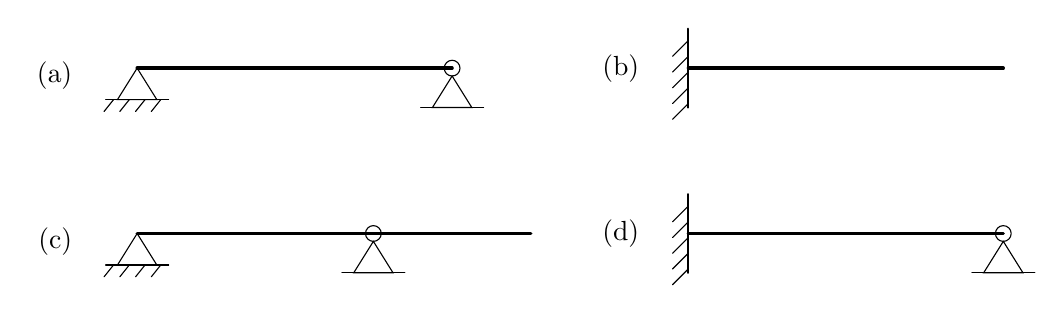
\begin{tikzpicture}[x=1cm,y=1cm,line cap=round,>=stealth]
    % ---------- (a) biapoiada ----------
    \begin{scope}[shift={(0,3.6)}]
      \draw[very thick] (0,0) -- (4,0);
      \draw (0,0) -- (-0.25,-0.4) -- (0.25,-0.4) -- cycle;
      \draw (-0.4,-0.4) -- (0.4,-0.4);
      \draw (4,0) circle (0.1);
      \draw (4,-0.1) -- (3.75,-0.5) -- (4.25,-0.5) -- cycle;
      \draw (3.6,-0.5) -- (4.4,-0.5);
      \foreach \x in {-0.3,-0.1,0.1,0.3}{\draw (\x,-0.4) -- (\x-0.12,-0.55);}
      \node[anchor=east] at (-0.7,-0.1) {(a)};
    \end{scope}
    % ---------- (b) engastada ----------
    \begin{scope}[shift={(7,3.6)}]
      \draw[very thick] (0,0) -- (4,0);
      \draw[thick] (0,-0.5) -- (0,0.5);
      \foreach \y in {-0.45,-0.25,-0.05,0.15,0.35}{\draw (0,\y) -- (-0.2,\y-0.2);}
      \node[anchor=east] at (-0.5,0) {(b)};
    \end{scope}
    % ---------- (c) balanço ----------
    \begin{scope}[shift={(0,1.5)}]
      \draw[very thick] (0,0) -- (5,0);
      \draw (0,0) -- (-0.25,-0.4) -- (0.25,-0.4) -- cycle;
      \draw (-0.4,-0.4) -- (0.4,-0.4);
      \draw (3,0) circle (0.1);
      \draw (3,-0.1) -- (2.75,-0.5) -- (3.25,-0.5) -- cycle;
      \draw (2.6,-0.5) -- (3.4,-0.5);
      \foreach \x in {-0.3,-0.1,0.1,0.3}{\draw (\x,-0.4) -- (\x-0.12,-0.55);}
      \node[anchor=east] at (-0.7,-0.1) {(c)};
    \end{scope}
    % ---------- (d) indeterminada ----------
    \begin{scope}[shift={(7,1.5)}]
      \draw[very thick] (0,0) -- (4,0);
      \draw[thick] (0,-0.5) -- (0,0.5);
      \foreach \y in {-0.45,-0.25,-0.05,0.15,0.35}{\draw (0,\y) -- (-0.2,\y-0.2);}
      \draw (4,0) circle (0.1);
      \draw (4,-0.1) -- (3.75,-0.5) -- (4.25,-0.5) -- cycle;
      \draw (3.6,-0.5) -- (4.4,-0.5);
      \node[anchor=east] at (-0.5,0) {(d)};
    \end{scope}
  \end{tikzpicture}
  \fonte{Adaptado de \citeonline{Norton2013}.}
\end{figure}

A viga engastada, em particular, é a idealização adotada neste trabalho para o conjunto
enrijecedor e linha flexível, conforme as premissas apresentadas no
Capítulo~\ref{sec:metodologia}, uma vez que o engaste modela a fixação da estrutura
na região de topo.

As cargas aplicadas a uma viga podem ser forças concentradas, forças distribuídas ao
longo de parte do comprimento ou do comprimento total, e momentos concentrados. Essas
cargas dão origem tanto a forças cortantes quanto a momentos fletores na viga, de
modo que a análise dos esforços internos consiste em determinar a magnitude e a
distribuição desses esforços ao longo do comprimento \cite{Norton2013}. Em
geral, as vigas são tratadas como sistemas estáticos, ainda que vibrações e acelerações
possam provocar carregamento dinâmico \cite{Norton2013}.

\subsection{Força Cortante e Momento Fletor}
\label{sub:cortante-momento}

Seja $q(x)$ a função que descreve o carregamento distribuído ao longo do eixo $x$ da
viga. A força cortante $V(x)$ e o momento fletor $M(x)$ relacionam-se com $q(x)$ por
\cite{Norton2013}:

\begin{equation}
  \label{eq:q-V-M}
  q(x) = \frac{\mathrm{d}V}{\mathrm{d}x} = \frac{\mathrm{d}^2 M}{\mathrm{d}x^2}.
\end{equation}

Integrando-se a Equação~(\ref{eq:q-V-M}) uma vez, obtém-se a força cortante e, uma
segunda vez, o momento fletor:

\begin{align}
  V(x) &= \int q(x)\,\mathrm{d}x + C_1, \label{eq:V-integral}\\
  M(x) &= \int V(x)\,\mathrm{d}x + C_1 x + C_2, \label{eq:M-integral}
\end{align}

em que $C_1$ e $C_2$ são constantes de integração, determinadas pelas condições de
contorno do problema \cite{Norton2013}. Em termos geométricos, a
diferença entre as forças cortantes em dois pontos quaisquer é igual à área sob a curva
do carregamento distribuído entre eles, e a diferença entre os momentos fletores em dois
pontos é igual à área sob a curva da força cortante \cite{Norton2013}.

Quanto à convenção de sinais, adota-se o momento fletor positivo quando ele coloca
a parte superior da viga em compressão e a parte inferior em tração, e a força
cortante positiva quando provoca uma rotação horária na seção em que atua
\cite{Norton2013}. Os valores máximos absolutos
de $V$ e $M$ são os de maior interesse, pois determinam as tensões críticas na viga.
Como $V$ é a derivada de $M$, o momento fletor atinge um máximo ou um mínimo nas
seções em que a força cortante se anula \cite{Norton2013}. Nas vigas
engastadas com carga na extremidade livre, a força cortante não se anula ao longo do
comprimento e o momento máximo ocorre no engaste, que é a seção crítica do projeto.

Para carregamentos formados por parcelas discretas, possivelmente descontínuas ao longo
do comprimento, é conveniente representar $q(x)$ por funções de singularidade, que
permitem escrever uma única expressão válida em toda a viga e facilitam a solução
computacional \cite{Norton2013}. Sob pequenas deflexões, vale também a
superposição de efeitos, de modo que casos combinados podem ser resolvidos somando-se
as soluções de casos individuais \cite{Norton2013}.

\subsection{Tensões Normais de Flexão}
\label{sub:tensoes-flexao}

Embora raramente uma viga real esteja sujeita à flexão pura, esse caso é o ponto de
partida para o desenvolvimento da teoria das tensões de flexão. Considere-se a viga
biapoiada da Figura~\ref{fig:flexao-pura}, com duas cargas idênticas aplicadas
simetricamente. No trecho entre as cargas a força cortante é nula e o momento
fletor é constante, caracterizando a flexão pura \cite{Norton2013}.

A dedução das tensões nesse regime baseia-se nas seguintes hipóteses
\cite{Norton2013}:

\begin{enumerate}
  \item o segmento analisado está distante das cargas aplicadas e dos vínculos externos;
  \item a viga é carregada em um plano de simetria;
  \item as seções transversais permanecem planas e perpendiculares à linha neutra
  durante a flexão;
  \item o material é homogêneo e obedece à lei de Hooke;
  \item as tensões permanecem abaixo do limite elástico e as deflexões são pequenas;
  \item o segmento está sujeito à flexão pura, sem cargas axiais ou cortantes;
  \item a viga é inicialmente reta.
\end{enumerate}

Essas hipóteses são as da teoria clássica de vigas de Euler-Bernoulli, adotada nas
premissas deste trabalho (Capítulo~\ref{sec:metodologia}).

\begin{figure}[h]
  \centering
  \caption{Flexão pura em uma viga biapoiada: (a) carregamento e reações;
    (b) diagrama de força cortante; (c) diagrama de momento fletor.}
  \label{fig:flexao-pura}
  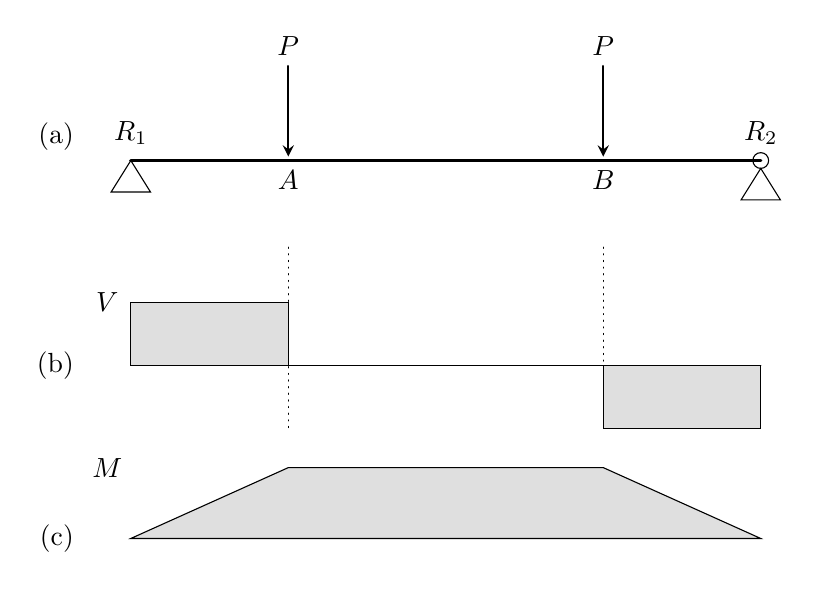
\begin{tikzpicture}[x=1cm,y=1cm,line cap=round,>=stealth]
    % --- (a) viga e cargas ---
    \draw[very thick] (0,0) -- (8,0);
    \draw (0,0) -- (-0.25,-0.4) -- (0.25,-0.4) -- cycle;
    \draw (8,-0.1) -- (7.75,-0.5) -- (8.25,-0.5) -- cycle;
    \draw (8,0) circle (0.1);
    \draw[->,thick] (2,1.2) -- (2,0.05);
    \draw[->,thick] (6,1.2) -- (6,0.05);
    \node at (2,1.45) {$P$};
    \node at (6,1.45) {$P$};
    \node at (2,-0.25) {$A$};
    \node at (6,-0.25) {$B$};
    \node at (0,0.35) {$R_1$};
    \node at (8,0.35) {$R_2$};
    \node[anchor=east] at (-0.6,0.3) {(a)};
    % --- (b) cortante ---
    \begin{scope}[shift={(0,-2.6)}]
      \draw[thin] (0,0) -- (8,0);
      \draw[fill=gray!25] (0,0) -- (0,0.8) -- (2,0.8) -- (2,0) -- cycle;
      \draw[fill=gray!25] (6,0) -- (6,-0.8) -- (8,-0.8) -- (8,0) -- cycle;
      \node at (-0.3,0.8) {$V$};
      \node[anchor=east] at (-0.6,0) {(b)};
      \draw[dotted] (2,1.5) -- (2,-0.8);
      \draw[dotted] (6,1.5) -- (6,-0.8);
    \end{scope}
    % --- (c) momento ---
    \begin{scope}[shift={(0,-4.8)}]
      \draw[thin] (0,0) -- (8,0);
      \draw[fill=gray!25] (0,0) -- (2,0.9) -- (6,0.9) -- (8,0) -- cycle;
      \node at (-0.3,0.9) {$M$};
      \node[anchor=east] at (-0.6,0) {(c)};
    \end{scope}
  \end{tikzpicture}
  \fonte{Adaptado de \citeonline{Norton2013}.}
\end{figure}

Quando o momento fletor é aplicado, o segmento se curva: as fibras de um dos lados
encurtam-se e ficam em compressão, as do lado oposto alongam-se e ficam em tração,
enquanto a linha neutra mantém o comprimento original. Para que as seções
permaneçam planas, a deformação varia linearmente com a distância à linha neutra, e,
sob a lei de Hooke, o mesmo ocorre com a tensão normal, que é nula na linha neutra
\cite{Norton2013}. Essa relação conduz à conhecida fórmula da tensão de
flexão:

\begin{equation}
  \label{eq:sigma-flexao}
  \sigma_x = -\frac{M y}{I},
\end{equation}

em que $M$ é o momento fletor na seção considerada, $I$ é o momento de inércia da área
da seção transversal em relação à linha neutra, que passa pelo centroide da seção
em uma viga reta, e $y$ é a distância da linha neutra ao ponto onde a tensão é
calculada \cite{Norton2013}. O sinal negativo resulta da convenção de sinais
adotada.

A tensão máxima ocorre nas fibras externas, onde $y = c$:

\begin{equation}
  \label{eq:sigma-max}
  \sigma_{max} = \frac{M c}{I},
\end{equation}

sendo $c$ a distância da linha neutra à fibra externa, tomada como positiva tanto
na parte superior quanto na inferior. Essas duas distâncias só são iguais em seções
simétricas em relação à linha neutra \cite{Norton2013}. Uma forma alternativa
frequentemente empregada é

\begin{equation}
  \label{eq:sigma-Z}
  \sigma_{max} = \frac{M}{Z}, \qquad Z = \frac{I}{c},
\end{equation}

em que $Z$ é o módulo de resistência da seção \cite{Norton2013}. A
Figura~\ref{fig:distribuicao-tensao} ilustra a distribuição linear da tensão normal ao
longo da altura da seção.

\begin{figure}[h]
  \centering
  \caption{Distribuição da tensão normal de flexão ao longo da altura de uma seção
    simétrica: tração em um lado, compressão no outro e tensão nula na linha neutra.}
  \label{fig:distribuicao-tensao}
  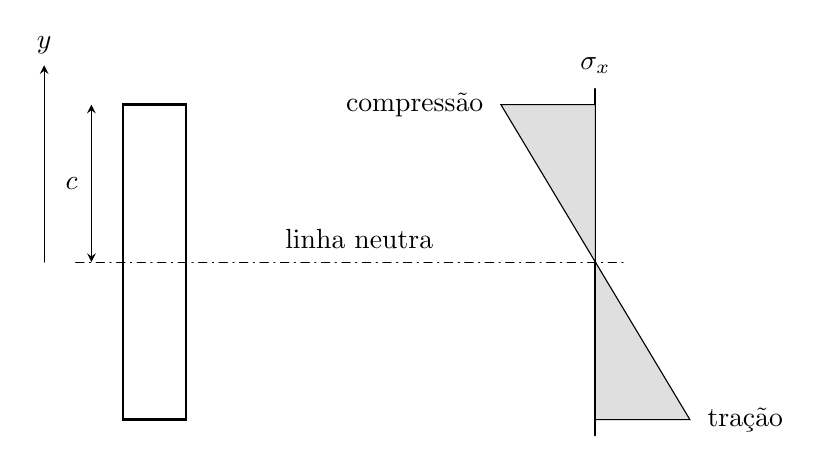
\begin{tikzpicture}[x=1cm,y=1cm,line cap=round,>=stealth]
    % seção (retângulo representando a altura da seção)
    \draw[thick] (0,-2) rectangle (0.8,2);
    % linha neutra
    \draw[dash dot] (-0.6,0) -- (6.4,0);
    \node at (3.0,0.3) {linha neutra};
    % eixo y e distância c
    \draw[->] (-1.0,0) -- (-1.0,2.5);
    \node at (-1.0,2.75) {$y$};
    \draw[<->] (-0.4,0) -- (-0.4,2);
    \node[anchor=east] at (-0.45,1) {$c$};
    % diagrama de tensões (triangular)
    \draw[thick] (6,2.2) -- (6,-2.2);
    \draw[fill=gray!25] (6,0) -- (6,2) -- (4.8,2) -- cycle;
    \draw[fill=gray!25] (6,0) -- (6,-2) -- (7.2,-2) -- cycle;
    \node[anchor=east] at (4.7,2.0) {compressão};
    \node[anchor=west] at (7.3,-2.0) {tração};
    \node at (6,2.5) {$\sigma_x$};
  \end{tikzpicture}
  \fonte{Adaptado de \citeonline{Norton2013}.}
\end{figure}

O momento de inércia $I$ depende exclusivamente da geometria da seção. Para um
retângulo de largura $b$ e altura $h$, $I = b h^3/12$ \cite{Norton2013}; para
uma seção circular maciça de diâmetro $d$, $I = \pi d^4/64$, e para uma seção
anular de diâmetros externo $D$ e interno $d$, $I = \pi (D^4 - d^4)/64$. A dependência
de $I$ com a quarta potência do diâmetro explica por que pequenas variações de
geometria alteram de modo significativo a rigidez e as tensões, aspecto central no
projeto de elementos de seção variável como o enrijecedor.

As Equações~(\ref{eq:sigma-flexao}) a (\ref{eq:sigma-Z}), embora deduzidas para
flexão pura, também podem ser utilizadas quando há outros carregamentos além do
momento fletor, desde que a deformação por cisalhamento seja desprezível
\cite{Norton2013}.

No caso de vigas curvas, isto é, de elementos com curvatura inicial significativa,
como ganchos e grampos, a linha neutra se desloca em direção ao centro de curvatura
e deixa de coincidir com a linha centroidal; a distribuição de tensões passa a ser
hiperbólica e não mais linear, e as Equações~(\ref{eq:sigma-flexao}) a
(\ref{eq:sigma-Z}) não se aplicam diretamente \cite{Norton2013}.
Como a hipótese de viga inicialmente reta é adotada neste trabalho, esse caso não é
desenvolvido aqui.

\subsection{Tensões de Cisalhamento na Flexão}
\label{sub:cisalhamento-flexao}

Na situação mais comum, a viga está submetida simultaneamente a força cortante e a
momento fletor. Como o momento varia com $x$ quando $V \neq 0$, as tensões normais nas
duas faces de um elemento da viga são diferentes, e o equilíbrio exige uma tensão de
cisalhamento compensatória \cite{Norton2013}. A tensão de cisalhamento
a uma distância $y_1$ da linha neutra é dada por \cite{Norton2013}:

\begin{equation}
  \label{eq:tau-flexao}
  \tau = \frac{V Q}{I b},
\end{equation}

em que $b$ é a largura da seção transversal em $y_1$ e $Q$ é o momento estático, em
relação à linha neutra, da porção da seção situada além de $y_1$:

\begin{equation}
  \label{eq:Q}
  Q = \int_{y_1}^{c} y\,\mathrm{d}A.
\end{equation}

Como $Q$ se anula na fibra externa e é máximo na linha neutra, a tensão de
cisalhamento devida à força cortante é nula na superfície e máxima na linha neutra,
ao contrário da tensão normal de flexão, que é nula na linha neutra e máxima na
superfície. Por isso, a combinação das duas tensões em um elemento qualquer da seção
raramente origina um estado de tensão pior do que o das fibras externas
\cite{Norton2013}. A Tabela~\ref{tab:tau-max} apresenta os valores máximos
da tensão de cisalhamento para algumas seções usuais, sendo $A$ a área da seção.

\begin{table}[h]
  \caption{Tensão máxima de cisalhamento devida à força cortante em vigas de
    diferentes seções transversais.}
  \label{tab:tau-max}
  \begin{center}
    \begin{tabular}{lc}
      \toprule
      Seção transversal                   & $\tau_{max}$ (na linha neutra)  \\
      \midrule
      Retangular                          & $\dfrac{3V}{2A}$                \\[2ex]
      Circular maciça                     & $\dfrac{4V}{3A}$                \\[2ex]
      Circular oca de parede fina         & $\dfrac{2V}{A}$                 \\[2ex]
      Viga I (aproximação pela alma)      & $\dfrac{V}{A_{alma}}$           \\
      \bottomrule
    \end{tabular}
  \end{center}
  \fonte{Adaptado de \citeonline{Norton2013}.}
  \nota{Para a seção circular oca, considera-se parede de espessura inferior a,
    aproximadamente, um décimo do raio externo.}
\end{table}

A tensão de cisalhamento devida à cortante é pequena em comparação com a tensão
normal de flexão quando a viga é longa em relação à sua altura. Como regra prática,
ela pode ser ignorada se a razão entre o comprimento e a altura da viga for igual
ou superior a 10; abaixo desse valor, a análise deve considerar ambas as tensões
\cite{Norton2013}.

\subsection{Deflexão em Vigas}
\label{sub:deflexao-vigas}

A teoria de Euler-Bernoulli considera que as seções transversais permanecem planas e
perpendiculares ao eixo deformado da viga. Isso significa desprezar a parcela da deflexão
causada pela deformação por cisalhamento, mas não a força cortante que participa do equilíbrio.
Quando essa parcela é relevante, uma teoria que a inclua, como a de \citeonline{Timoshenko1921}, permite
considerar separadamente a rotação da seção e a inclinação do eixo. A escolha depende da
geometria e das rigidezes à flexão e ao cisalhamento, não apenas da comparação entre tensões.
Para o conjunto linha flexível-enrijecedor, \citeonline{Caire2011} discute avaliações
nas quais a inclusão do cisalhamento teve pouca influência na distribuição de curvatura.
Além disso, a hipótese de Euler-Bernoulli não deve ser confundida com a aproximação de
pequenas rotações utilizada na equação de deflexão apresentada a seguir.

Além das tensões, o projetista deve considerar a deflexão, pois, mesmo com tensões
bem abaixo dos níveis de falha do material, as deflexões elásticas podem causar
interferências e desalinhamentos em um sistema \cite{Norton2013}. A deflexão
por flexão é obtida a partir da equação da viga
\cite{Norton2013}:

\begin{equation}
  \label{eq:viga-EI}
  \frac{\mathrm{d}^2 y}{\mathrm{d}x^2} = \frac{M(x)}{E I},
\end{equation}

em que $y(x)$ é a deflexão, $E$ é o módulo de elasticidade do material e $I$ é o
momento de inércia da seção. O produto $E I$ é a rigidez à flexão da viga. A
Equação~(\ref{eq:viga-EI}) é válida somente para pequenas deflexões e não inclui o
efeito da força cortante, que em vigas longas é normalmente desprezado, a menos que a
razão entre comprimento e altura seja inferior a, aproximadamente, 10
\cite{Norton2013}.

Derivando-se a Equação~(\ref{eq:viga-EI}) duas vezes e integrando-se duas vezes,
obtém-se o conjunto de equações que descreve o comportamento da viga
\cite{Norton2013}:

\begin{align}
  \frac{q}{E I} &= \frac{\mathrm{d}^4 y}{\mathrm{d}x^4}, \label{eq:viga-q}\\
  \frac{V}{E I} &= \frac{\mathrm{d}^3 y}{\mathrm{d}x^3}, \label{eq:viga-V}\\
  \frac{M}{E I} &= \frac{\mathrm{d}^2 y}{\mathrm{d}x^2}, \label{eq:viga-M}\\
  \theta        &= \frac{\mathrm{d}y}{\mathrm{d}x}, \label{eq:viga-theta}\\
  y             &= f(x), \label{eq:viga-y}
\end{align}

em que $\theta$ é a rotação da seção. O único parâmetro de material nessas equações é o
módulo de elasticidade $E$, que define a rigidez do material \cite{Norton2013}.
A determinação da função de deflexão é, portanto, um exercício de integração: a função
de carregamento $q$ é normalmente conhecida e as constantes de integração são obtidas
a partir das condições de contorno da configuração particular da viga
\cite{Norton2013}. Para uma viga engastada em $x = 0$, por exemplo, as
condições de contorno são deflexão e rotação nulas no engaste, $y(0) = 0$ e
$\theta(0) = 0$, e momento fletor e força cortante nulos na extremidade livre.

Quando a seção transversal varia ao longo do comprimento, o produto $E I$ deixa de
ser constante e passa a ser uma função $E I(x)$. Nesse caso, é necessário construir
a função $M/EI$ a partir do diagrama de momento antes de integrar, e a integração
deve ser feita por trechos para considerar as variações de $I$
\cite{Norton2013}. Esse é o caso do enrijecedor à flexão, cuja geometria
cônica faz com que $I$ decresça com $x$. Além disso, ao se considerar o
comportamento viscoelástico do poliuretano, o módulo de elasticidade $E$ deixa de ser
uma constante e passa a depender do tempo, conforme discutido na
Seção~\ref{sec:viscoelasticidade} e na Subseção~\ref{sub:rigidez}.

% ---------------------------------------------------------------------

\section{Viscoelasticidade}
\label{sec:viscoelasticidade}

Em um sólido elástico linear, a tensão é proporcional à deformação e independe do
tempo, relação expressa pela lei de Hooke, $\sigma = E\,\varepsilon$, em que $E$ é o
módulo de elasticidade \cite{Caire2005}. Diversos materiais, porém, apresentam
tensão e deformação dependentes do tempo; essa característica é denominada
viscoelasticidade e é bastante comum, à temperatura ambiente, em materiais poliméricos
como o poliuretano \cite{Caire2005}. Esta seção apresenta os fenômenos de
fluência e relaxação, os modelos mecânicos que os descrevem, a equação constitutiva
na forma integral, a resposta em regime harmônico e os limites da teoria linear. Em
seguida, na Subseção~\ref{sub:rigidez}, esses conceitos são aplicados à rigidez à flexão
do conjunto linha flexível-enrijecedor. As funções constitutivas são tratadas aqui
em sua forma geral; sua representação por série de Prony é apresentada na
Subseção~\ref{subsec:serie-prony} e o procedimento de ajuste aos dados experimentais, na
Seção~\ref{sec:caracterizacao-do-material}.

\subsection{Fluência e Relaxação de Tensão}
\label{sub:fluencia-relaxacao}

A resposta mecânica de um sólido viscoelástico reúne aspectos de um sólido elástico e de
um fluido viscoso \cite{Caire2005}. Quando uma tensão é aplicada
instantaneamente e mantida constante, observa-se uma deformação instantânea,
característica de um sólido elástico, seguida de uma deformação continuada a taxa não
constante, denominada fluência \cite{Caire2005}. De modo análogo, quando uma
deformação é imposta em $t = 0$ e mantida constante, a tensão sofre um salto e decai
gradualmente com o tempo, fenômeno denominado relaxação de tensão. Sólidos elásticos
mantêm a tensão constante e não apresentam essa característica, enquanto fluidos
newtonianos relaxam a tensão instantaneamente \cite{Caire2005}. A
Figura~\ref{fig:fluencia-relaxacao} ilustra as duas respostas.

\begin{figure}[h]
  \centering
  \caption{Respostas características de um material viscoelástico: relaxação de tensão,
    (a) deformação imposta e (b) tensão resultante; e fluência, (c) tensão imposta e
    (d) deformação resultante.}
  \label{fig:fluencia-relaxacao}
  \begin{tikzpicture}[x=1cm,y=1cm,line cap=round,>=stealth]
    % ---------- (a) deformacao imposta (relaxacao) ----------
    \begin{scope}[shift={(0,3.6)}]
      \draw[->] (0,0) -- (4.2,0) node[right] {$t$};
      \draw[->] (0,0) -- (0,2.3) node[above] {$\varepsilon$};
      \draw[very thick] (0,1.4) -- (3.9,1.4);
      \draw[dotted] (0,0) -- (0,1.4);
      \node[anchor=east] at (0,1.4) {$\varepsilon_0$};
      \node[anchor=north west] at (0.1,2.3) {(a)};
    \end{scope}
    % ---------- (b) tensao resultante ----------
    \begin{scope}[shift={(0,0)}]
      \draw[->] (0,0) -- (4.2,0) node[right] {$t$};
      \draw[->] (0,0) -- (0,2.6) node[above] {$\sigma$};
      \draw[very thick,domain=0:3.9,samples=40,smooth,variable=\x]
        plot ({\x},{0.9+1.2*exp(-\x/0.9)});
      \draw[dashed] (0,0.9) -- (3.9,0.9);
      \node[anchor=east] at (0,2.1) {$\varepsilon_0 G(0)$};
      \node[anchor=east] at (0,0.9) {$\varepsilon_0 G_{\infty}$};
      \node[anchor=north west] at (0.1,2.6) {(b)};
    \end{scope}
    % ---------- (c) tensao imposta (fluencia) ----------
    \begin{scope}[shift={(8,3.6)}]
      \draw[->] (0,0) -- (4.2,0) node[right] {$t$};
      \draw[->] (0,0) -- (0,2.3) node[above] {$\sigma$};
      \draw[very thick] (0,1.4) -- (3.9,1.4);
      \draw[dotted] (0,0) -- (0,1.4);
      \node[anchor=east] at (0,1.4) {$\sigma_0$};
      \node[anchor=north west] at (0.1,2.3) {(c)};
    \end{scope}
    % ---------- (d) deformacao resultante ----------
    \begin{scope}[shift={(8,0)}]
      \draw[->] (0,0) -- (4.2,0) node[right] {$t$};
      \draw[->] (0,0) -- (0,2.6) node[above] {$\varepsilon$};
      \draw[very thick,domain=0:3.9,samples=40,smooth,variable=\x]
        plot ({\x},{2.0-1.2*exp(-\x/0.9)});
      \draw[dashed] (0,2.0) -- (3.9,2.0);
      \node[anchor=east] at (0,0.8) {$\sigma_0 J(0)$};
      \node[anchor=east] at (0,2.0) {$\sigma_0 J_{\infty}$};
      \node[anchor=north west] at (0.1,2.6) {(d)};
    \end{scope}
  \end{tikzpicture}
  \fonte{Adaptado de \citeonline{Caire2005}.}
\end{figure}

Os ensaios usuais para caracterizar essa resposta são o de fluência, em que se aplicam
tensões constantes a corpos de prova e se mede a deformação ao longo do tempo, e o de
relaxação, em que se impõem deformações constantes e se mede a tensão \cite{Caire2005}.
No caso do comportamento viscoelástico linear, as funções que caracterizam o material
são a função de relaxação $G(t)$ e a função de fluência $J(t)$, definidas por
\cite{Caire2005}

\begin{equation}
  \label{eq:ve-G-J}
  G(t) = \frac{\sigma(t)}{\varepsilon_0}, \qquad
  J(t) = \frac{\varepsilon(t)}{\sigma_0},
\end{equation}

em que $\varepsilon_0$ é a deformação constante imposta no ensaio de relaxação e
$\sigma_0$ é a tensão constante imposta no ensaio de fluência. Como $\sigma$ e $\varepsilon$ são tensão e deformação normais, $G(t)$ é um módulo de
relaxação longitudinal, e não o módulo de cisalhamento, e a letra $G$ segue a notação de
\citeonline{Caire2011}. Essas funções cumprem,
para o material viscoelástico linear, o papel que o módulo de elasticidade cumpre para o
sólido elástico \cite{Caire2005}.

A viscoelasticidade é linear quando vale o princípio da superposição linear: a resposta
a uma história de tensão multiplicada por uma constante $C$ é a resposta original
multiplicada por $C$, e a resposta à soma de duas histórias de tensão, a segunda
aplicada com atraso $t_1$, é a soma das respostas individuais \cite{Caire2005}.
Denotando por $\mathcal{E}[\,\cdot\,]$ a deformação resultante de um histórico de tensão,

\begin{align}
  \mathcal{E}\left[C\,\sigma(t)\right] &= C\,\mathcal{E}\left[\sigma(t)\right],
    \label{eq:ve-superposicao}\\
  \mathcal{E}\left[\sigma_1(t) + \sigma_2(t - t_1)\right]
  &= \mathcal{E}\left[\sigma_1(t)\right] + \mathcal{E}\left[\sigma_2(t - t_1)\right].
\end{align}

\subsection{Modelos Mecânicos}
\label{sub:modelos-mecanicos}

Para simular as propriedades de estruturas poliméricas, recorre-se a modelos mecânicos
formados por dois elementos fundamentais: a mola linear, que representa o sólido
elástico, $\sigma = E\,\varepsilon$, e o amortecedor linear, que representa o fluido
viscoso, $\sigma = \mu\,\dot{\varepsilon}$, em que $\mu$ é a viscosidade e o ponto
indica derivada em relação ao tempo \cite{Caire2005}. Cada combinação desses
elementos conduz a uma equação constitutiva com operador diferencial linear, e os modelos
diferem apenas na forma das funções $G(t)$ e $J(t)$. Embora alguns sejam mais
representativos, nenhum deles fornece, por si só, uma previsão adequada da resposta
viscoelástica do poliuretano, e por isso o procedimento adequado é ajustar a função $G(t)$
ou $J(t)$ a dados experimentais do material específico \cite{Caire2005}.

No modelo de Maxwell, uma mola e um amortecedor são associados em série: a tensão é a
mesma nos dois elementos e a deformação total é a soma das deformações individuais, de
modo que \cite{Caire2005}

\begin{equation}
  \label{eq:ve-maxwell}
  \dot{\varepsilon} = \frac{\dot{\sigma}}{E} + \frac{\sigma}{\mu}.
\end{equation}

Em um ensaio de relaxação, com $\dot{\varepsilon} = 0$, a tensão decai
exponencialmente, $\sigma(t) = \sigma_0\,e^{-t/\tau_R}$, com tempo de relaxação
$\tau_R = \mu/E$, e a função de relaxação resulta em $G(t) = E\,e^{-t/\tau_R}$
\cite{Caire2005}. Em um ensaio de fluência, com $\dot{\sigma} = 0$, obtém-se
$\varepsilon(t) = \sigma_0\left(1/E + t/\mu\right)$ e, portanto,
$J(t) = \left(1 + t/\tau_R\right)/E$ \cite{Caire2005}. A deformação cresce
linearmente, sem limite, como em um fluido, razão pela qual o modelo não representa o
comportamento observado em polímeros reais \cite{Caire2005}.

No modelo de Kelvin-Voigt, a mola e o amortecedor são associados em paralelo: a
deformação é a mesma nos dois elementos e a tensão é a soma das tensões individuais
\cite{Caire2005},

\begin{equation}
  \label{eq:ve-kelvin}
  \sigma = E\,\varepsilon + \mu\,\dot{\varepsilon}.
\end{equation}

Sob tensão constante $\sigma_0$, a integração da Equação~(\ref{eq:ve-kelvin}) fornece
$\varepsilon(t) = \left(\sigma_0/E\right)\left(1 - e^{-t/\tau_C}\right)$, em que
$\tau_C = \mu/E$ é o tempo de retardo, de modo que
$J(t) = \left(1 - e^{-t/\tau_C}\right)/E$ \cite{Caire2005}. Sob deformação
constante, porém, a equação se reduz a $\sigma = E\,\varepsilon$, isto é, a tensão
permanece constante e o material responde como um sólido elástico, o que torna o modelo
inadequado como representação geral do comportamento viscoelástico \cite{Caire2005}.

O modelo do sólido linear padrão é formado por um elemento de Maxwell, com mola $E_m$ e
amortecedor $\mu$, associado em paralelo a uma mola $E_a$ \cite{Caire2005}. A
equação constitutiva resultante é

\begin{equation}
  \label{eq:ve-sls}
  \frac{\dot{\sigma}}{E_m} + \frac{\sigma}{\mu}
  = \left(1 + \frac{E_a}{E_m}\right)\dot{\varepsilon} + \frac{E_a}{\mu}\,\varepsilon,
\end{equation}

e sua resposta de relaxação é $G(t) = E_a + E_m\,e^{-t/\tau_R}$, com
$\tau_R = \mu/E_m$ \cite{Caire2005}. Para fluência, a função
$J(t)$ parte de $J(0) = 1/(E_a + E_m)$ e tende a $J(\infty) = 1/E_a$ com tempo de retardo
$\tau_C = \mu\,(E_a + E_m)/(E_a E_m)$ \cite{Caire2005}. Esse é o modelo mais
simples capaz de representar, de forma aproximada, todas as características observadas
no comportamento de sólidos viscoelásticos, e pode ser usado na falta de dados
experimentais \cite{Caire2005}. A Tabela~\ref{tab:modelos-mecanicos} reúne as
equações dos três modelos. A relaxação do sólido linear padrão, com um único termo
exponencial somado a um valor de longo prazo, é o caso mais simples da série de Prony
apresentada na Subseção~\ref{subsec:serie-prony}.

\begin{table}[h]
  \caption{Equações constitutivas e funções de relaxação e de fluência de modelos
    mecânicos viscoelásticos lineares.}
  \label{tab:modelos-mecanicos}
  \begin{center}
    \footnotesize
    \begin{tabular}{p{2.2cm}p{4.6cm}p{3.0cm}p{4.2cm}}
      \toprule
      Modelo & Equação constitutiva & Relaxação $G(t)$ & Fluência $J(t)$ \\
      \midrule
      Maxwell
        & $\dot{\varepsilon} = \dfrac{\dot{\sigma}}{E} + \dfrac{\sigma}{\mu}$
        & $E\,e^{-t/\tau_R}$, $\tau_R = \dfrac{\mu}{E}$
        & $\dfrac{1}{E}\left(1 + \dfrac{t}{\tau_R}\right)$ \\[3ex]
      Kelvin-Voigt
        & $\sigma = E\,\varepsilon + \mu\,\dot{\varepsilon}$
        & Não relaxa: $\sigma = E\,\varepsilon$
        & $\dfrac{1}{E}\left(1 - e^{-t/\tau_C}\right)$, $\tau_C = \dfrac{\mu}{E}$ \\[3ex]
      Sólido linear padrão
        & $\dfrac{\dot{\sigma}}{E_m} + \dfrac{\sigma}{\mu} =
           \left(1 + \dfrac{E_a}{E_m}\right)\dot{\varepsilon} + \dfrac{E_a}{\mu}\,\varepsilon$
        & $E_a + E_m\,e^{-t/\tau_R}$, $\tau_R = \dfrac{\mu}{E_m}$
        & $J_{\infty} - \left(J_{\infty} - J_0\right)e^{-t/\tau_C}$, com
          $J_0 = \dfrac{1}{E_a + E_m}$, $J_{\infty} = \dfrac{1}{E_a}$ e
          $\tau_C = \dfrac{\mu\,(E_a + E_m)}{E_a E_m}$ \\
      \bottomrule
    \end{tabular}
  \end{center}
  \fonte{Adaptado de \citeonline{Caire2005}.}
  \nota{As funções $G(t)$ e $J(t)$ do sólido linear padrão foram reescritas
    explicitamente a partir de sua equação constitutiva.}
\end{table}

O modelo de Maxwell generalizado associa em paralelo uma mola isolada, de módulo
$G_{\infty}$, e $N$ elementos de Maxwell, cada um formado por uma mola $G_m$ e um
amortecedor $\mu_m$ em série (Figura~\ref{fig:maxwell-generalizado}). Como os ramos estão
em paralelo, a tensão total é a soma das tensões dos ramos e, sob deformação constante, a
função de relaxação é a soma das relaxações individuais: a mola isolada contribui com o
valor de longo prazo $G_{\infty}$, e o ramo $m$, com $G_m\,e^{-t/\tau_m}$, em que
$\tau_m = \mu_m/G_m$. O resultado é a série de Prony da
Equação~(\ref{eq:prony-relaxacao}) \cite{Caire2011}, de modo que essa série corresponde à
relaxação de um modelo de Maxwell generalizado, do qual o sólido linear padrão é o caso
$N = 1$. Cada termo representa uma escala de tempo de relaxação distinta.

\begin{figure}[h]
  \centering
  \caption{Modelo de Maxwell generalizado: uma mola isolada, de módulo $G_{\infty}$, em
    paralelo com $N$ elementos de Maxwell, cada um formado por uma mola $G_m$ e um
    amortecedor $\mu_m$ em série.}
  \label{fig:maxwell-generalizado}
  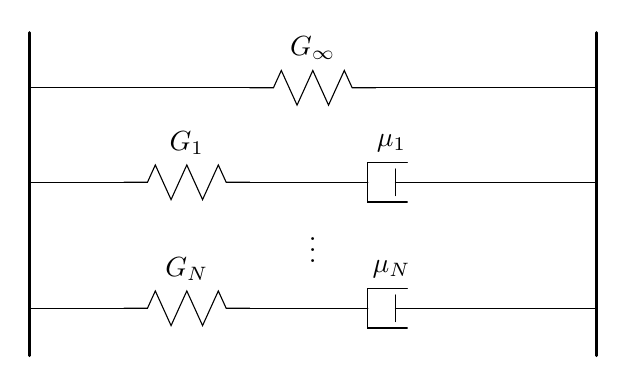
\begin{tikzpicture}[x=1cm,y=1cm,line cap=round,>=stealth,
      mola/.pic={\draw (0,0) -- (0.3,0) -- (0.4,0.22) -- (0.6,-0.22) -- (0.8,0.22)
        -- (1.0,-0.22) -- (1.2,0.22) -- (1.3,0) -- (1.6,0);},
      amort/.pic={\draw (0,0) -- (0.5,0); \draw (1.0,0.25) -- (0.5,0.25)
        -- (0.5,-0.25) -- (1.0,-0.25); \draw (0.85,0.17) -- (0.85,-0.17);
        \draw (0.85,0) -- (1.6,0);}]
    % barramentos
    \draw[very thick] (0,0.7) -- (0,-3.4);
    \draw[very thick] (7.2,0.7) -- (7.2,-3.4);
    % mola isolada
    \draw (0,0) -- (2.8,0);
    \pic at (2.8,0) {mola};
    \draw (4.4,0) -- (7.2,0);
    \node at (3.6,0.5) {$G_{\infty}$};
    % ramo 1
    \draw (0,-1.2) -- (1.2,-1.2);
    \pic at (1.2,-1.2) {mola};
    \draw (2.8,-1.2) -- (3.8,-1.2);
    \pic at (3.8,-1.2) {amort};
    \draw (5.4,-1.2) -- (7.2,-1.2);
    \node at (2.0,-0.7) {$G_1$};
    \node at (4.6,-0.7) {$\mu_1$};
    % reticencias
    \node at (3.6,-1.95) {$\vdots$};
    % ramo N
    \draw (0,-2.8) -- (1.2,-2.8);
    \pic at (1.2,-2.8) {mola};
    \draw (2.8,-2.8) -- (3.8,-2.8);
    \pic at (3.8,-2.8) {amort};
    \draw (5.4,-2.8) -- (7.2,-2.8);
    \node at (2.0,-2.3) {$G_N$};
    \node at (4.6,-2.3) {$\mu_N$};
  \end{tikzpicture}
  \fonte{Elaborada pelos autores.}
\end{figure}

\subsection{Equação Constitutiva na Forma Integral}
\label{sub:forma-integral}

Os modelos mecânicos descrevem a resposta por meio de equações diferenciais. Uma forma
mais geral, que utiliza diretamente a função de relaxação $G(t)$ ou a de fluência $J(t)$
obtida experimentalmente, é a equação constitutiva na forma integral, deduzida a partir
do princípio da superposição de Boltzmann \cite{Caire2011}. Se uma deformação
$\varepsilon(\tau) = \varepsilon_0\,1(\tau)$, com $1(\tau)$ a função degrau unitário, é
aplicada ao material, a tensão resultante é $\sigma(t) = \varepsilon_0\,G(t)$. Uma
história de deformação arbitrária, com variação suave no tempo, pode ser aproximada por
uma sucessão de saltos de deformação, e, segundo o princípio da superposição de
Boltzmann, a tensão total é a soma das respostas individuais a cada salto
\cite{Caire2011}. Fazendo o número de saltos tender ao infinito, a soma se
transforma em uma integral e obtém-se, para uma história de deformação $\varepsilon(\tau)$
\cite{Caire2011},

\begin{align}
  \sigma(t) &= \varepsilon(0)\,G(t)
  + \int_0^t G(t - \tau)\,\frac{\partial \varepsilon(\tau)}{\partial \tau}\,\mathrm{d}\tau
  \nonumber\\
  &= G(0)\,\varepsilon(t)
  + \int_0^t \frac{\partial G(t - \tau)}{\partial (t - \tau)}\,\varepsilon(\tau)\,\mathrm{d}\tau,
  \label{eq:ve-relaxacao-integral}
\end{align}

em que a segunda igualdade resulta de integração por partes e é a forma empregada na
formulação do enrijecedor (Subseção~\ref{sub:rigidez}). Como a tensão em um instante
depende de toda a história de deformação anterior, a integral representa a memória do
material. Procedimento análogo, partindo de um histórico de tensão, fornece a resposta de
deformação em função da função de fluência \cite{Caire2011}:

\begin{equation}
  \label{eq:ve-fluencia-integral}
  \varepsilon(t) = \sigma(0)\,J(t)
  + \int_0^t J(t - \tau)\,\frac{\partial \sigma(\tau)}{\partial \tau}\,\mathrm{d}\tau.
\end{equation}

O ensaio costuma fornecer apenas uma das duas funções, de relaxação ou de fluência, e, se
a formulação utiliza a outra, é necessário convertê-las. Substituindo-se um histórico de
tensão degrau na equação de relaxação, obtém-se a relação \cite{Caire2011}

\begin{equation}
  \label{eq:ve-relacao-G-J}
  1 = J(0)\,G(t) + \int_0^t G(t - \tau)\,\frac{\partial J(\tau)}{\partial \tau}\,\mathrm{d}\tau,
\end{equation}

que pode ser resolvida numericamente para a função desconhecida, e da qual decorrem
$G(0)\,J(0) = 1$ e $G(\infty)\,J(\infty) = 1$ \cite{Caire2011}. Neste trabalho
adota-se a função de relaxação, decomposta em uma parcela independente do tempo e uma
parcela decrescente \cite{Caire2011},

\begin{equation}
  \label{eq:ve-G-decomposicao}
  G(t) = G_{\infty} + \Delta G(t),
\end{equation}

em que $G_{\infty} = G(\infty)$ é o módulo de longo prazo e $\Delta G(t)$ é descrita pela
série de Prony da Equação~(\ref{eq:prony-relaxacao}), de modo que
$G(0) = G_{\infty} + \sum_{m} G_m$. O sólido linear padrão da
Subseção~\ref{sub:modelos-mecanicos}, com $G_{\infty} = E_a$ e um termo de amplitude
$E_m$, é o caso particular com $N = 1$.

\subsection{Resposta em Regime Harmônico}
\label{sub:regime-harmonico}

Em muitas aplicações de engenharia, a estrutura viscoelástica é submetida a
carregamentos harmônicos por longos períodos, e é mais conveniente reescrever as
equações diretamente no domínio da frequência \cite{Caire2011}. Considere-se o
histórico de deformação

\begin{equation}
  \label{eq:ve-def-harmonica}
  \varepsilon(t) = \varepsilon_0 + \Delta\varepsilon\,\sin\omega t,
\end{equation}

em que $\varepsilon_0$ é o valor médio, $\Delta\varepsilon$ é a amplitude da variação em
torno dele e $\omega$ é a frequência de carregamento \cite{Caire2011}.
Substituindo-se a Equação~(\ref{eq:ve-def-harmonica}) na Equação~(\ref{eq:ve-relaxacao-integral})
e considerando $t \to \infty$, de modo que a parcela transitória desapareça, a tensão
depende apenas da frequência \cite{Caire2011}:

\begin{align}
  \sigma(t) &= \varepsilon_0\,G_{\infty}
  + \Delta\varepsilon\left[G'(\omega)\sin\omega t + G''(\omega)\cos\omega t\right]
  \nonumber\\
  &= \varepsilon_0\,G_{\infty}
  + \Delta\varepsilon\left[G'(\omega)^2 + G''(\omega)^2\right]^{1/2}
  \sin\left(\omega t + \delta(\omega)\right),
  \label{eq:ve-tensao-harmonica}
\end{align}

com $\tan\delta(\omega) = G''(\omega)/G'(\omega)$. Os módulos $G'(\omega)$ e $G''(\omega)$ são
os limites, para $t \to \infty$, de \cite{Caire2011}

\begin{align}
  G'(\omega) &= G(0) + \int_0^{\infty} \cos(\omega\tau)\,
  \frac{\partial \Delta G(\tau)}{\partial \tau}\,\mathrm{d}\tau,
  \label{eq:ve-G-linhas}\\
  G''(\omega) &= -\int_0^{\infty} \sin(\omega\tau)\,
  \frac{\partial \Delta G(\tau)}{\partial \tau}\,\mathrm{d}\tau,
\end{align}

e são denominados módulo de armazenamento e módulo de perda, respectivamente. Para a série
de Prony, essas integrais conduzem às expressões das Equações~(\ref{eq:modulo-armazenamento})
e (\ref{eq:modulo-perda}). A resposta de tensão a uma deformação senoidal oscila na mesma
frequência $\omega$, com uma diferença de fase $\delta(\omega)$ em relação à deformação
\cite{Caire2011}. Para um histórico cossenoidal,
$\varepsilon(t) = \varepsilon_0 + \Delta\varepsilon\cos\omega t$, tem-se
$\sigma(t) = \varepsilon_0\,G_{\infty} + \Delta\varepsilon\left[G'(\omega)\cos\omega t
- G''(\omega)\sin\omega t\right]$ \cite{Caire2011}.

O módulo de armazenamento está associado à parcela da resposta em fase com a deformação,
isto é, ao armazenamento e à recuperação de energia elástica, e o módulo de perda, à
parcela defasada de $90^{\circ}$, associada à dissipação. O trabalho realizado por unidade
de volume durante um ciclo de deformação é

\begin{equation}
  \label{eq:ve-trabalho-ciclo}
  W_T = \int_0^{2\pi/\omega} \sigma(t)\,\dot{\varepsilon}(t)\,\mathrm{d}t
  = \pi\,(\Delta\varepsilon)^2\,G''(\omega),
\end{equation}

em que apenas o módulo de perda aparece, pois a parcela associada a $G'(\omega)$ se anula
no ciclo \cite{Caire2011}. Como o enrijecedor está sujeito a carregamentos
oscilatórios durante a operação, ele dissipa energia por seu comportamento viscoelástico,
e o efeito dessa dissipação sobre a curvatura e a deformação ao longo do comprimento deve
ser avaliado no projeto \cite{Caire2011}.

\subsection{Limites de Aplicação da Teoria Linear}
\label{sub:limites-linear}

A relativa simplicidade da viscoelasticidade linear leva a que muitos componentes
poliméricos sejam modelados por ela, mas uma grande parte dos polímeros apresenta
comportamento não linear mesmo para pequenas tensões, deformações e tempos, e o uso da
teoria linear em um material fortemente não linear pode causar erros graves de análise e
projeto \cite{Caire2011}. Um material é considerado linear se a tensão é
proporcional à deformação para um dado tempo e se o princípio da superposição é válido
\cite{Caire2011}. A validade da teoria depende das condições de ensaio e é
bastante afetada pela temperatura, pela umidade e pela taxa de deformação, e a transição
do comportamento linear para o não linear é progressiva, sem um procedimento padrão bem
definido para determiná-la \cite{Caire2011}. Como ordem de grandeza, polímeros
amorfos, em uma faixa de temperatura, mostram comportamento linear somente para
deformações abaixo de cerca de 1\%, e polímeros cristalinos, para deformações ainda
menores \cite{Caire2005}. Quando essa faixa é excedida, são necessárias teorias
não lineares, como as de Leaderman e de Green-Rivlin e o princípio da superposição
modificado, descritas por \citeonline{Caire2011}; este último é apresentado na
Subseção~\ref{sub:psm}. A adequação da hipótese
linear ao poliuretano nas condições estudadas, bem como o seu enquadramento nas premissas
do modelo (Seção~\ref{sec:premissas-adotadas}), deve, portanto, ser verificada com os
ensaios de caracterização.

\subsection{Princípio da Superposição Modificado}
\label{sub:psm}

Na viscoelasticidade linear, a tensão resultante de uma história de deformação é a
superposição das respostas a saltos de deformação, e cada resposta é proporcional ao
tamanho do salto. Fora do regime linear, essa proporcionalidade deixa de valer. O princípio
da superposição modificado (PSM) mantém a ideia de superpor as respostas aos saltos, mas
descreve a resposta a cada salto por uma função não linear da deformação e do tempo
decorrido desde sua aplicação \cite{Caire2011}. Fazendo o número de saltos tender ao
infinito, a soma se transforma em uma integral e obtém-se a forma constitutiva de
\citeonline{PipkinRogers1968}. Para representar a dependência não linear da tensão em
relação à deformação, expande-se a resposta em um polinômio de quarta ordem na
deformação, com uma função de relaxação $G_k(t)$ para cada potência $\varepsilon^k$
\cite{Caire2011}:

\begin{equation}
  \label{eq:ve-psm}
  \sigma(t) = \sum_{k=1}^{4} G_k(t)\,\varepsilon(0)^k
  + \int_0^t \Big[G_1(t-\tau) + 2G_2(t-\tau)\,\varepsilon(\tau)
  + 3G_3(t-\tau)\,\varepsilon(\tau)^2 + 4G_4(t-\tau)\,\varepsilon(\tau)^3\Big]
  \frac{\partial \varepsilon(\tau)}{\partial \tau}\,\mathrm{d}\tau.
\end{equation}

Quando $G_2 = G_3 = G_4 = 0$, a Equação~(\ref{eq:ve-psm}) se reduz à primeira forma da
Equação~(\ref{eq:ve-relaxacao-integral}), e $G_1(t)$ é a função de relaxação linear. Em um
ensaio de relaxação, com deformação constante $\varepsilon_i$ imposta em $t = 0$, o termo
integral se anula e a tensão é $\sigma_i(t) = \sum_{k=1}^{4} G_k(t)\,\varepsilon_i^k$
\cite{Caire2011}. Essa relação permite obter as funções $G_k(t)$ ajustando as curvas de
tensão medidas para diferentes níveis de deformação, e cada $G_k(t)$ pode ser descrita por
uma série de Prony com os mesmos tempos de relaxação \cite{Caire2011}. A identificação dos
coeficientes a partir dos ensaios é apresentada na
Subseção~\ref{sec:identificacao-funcoes-relaxacao}. A formulação estrutural deste trabalho
utiliza apenas a parcela linear, $G_1(t)$ (Subseção~\ref{sec:parametros-material-linear}).

\subsection{Rigidez}
\label{sub:rigidez}

Na Seção~\ref{sec:flexao}, a rigidez à flexão foi tratada como o produto $EI$, com módulo
de elasticidade $E$ constante. Quando parte da seção é de material viscoelástico, como
o poliuretano do enrijecedor, essa rigidez deixa de ser constante e passa a depender do
tempo ou da frequência. Considera-se, como hipótese simplificadora, que a resposta
viscoelástica é simétrica em tração e compressão; nesse caso, o eixo neutro passa pelo
centroide da área da seção para qualquer instante \cite{Caire2011}, premissa
adotada na Seção~\ref{sec:premissas-adotadas}. Sendo $\eta$ a distância ao eixo
neutro, a deformação é proporcional à curvatura, $\varepsilon(\eta, s, t) = \eta\,k(s,t)$,
e o equilíbrio de momentos na seção, somando-se as contribuições do duto flexível
(índice $PIPE$) e do enrijecedor (índice $BS$), é \cite{Caire2011}

\begin{equation}
  \label{eq:ve-M-tensoes}
  M(s,t) = \int_{A_{PIPE}} \sigma_{PIPE}\,\eta\,\mathrm{d}A
  + \int_{A_{BS}} \sigma_{BS}\,\eta\,\mathrm{d}A.
\end{equation}

Adotando-se para o enrijecedor a equação constitutiva integral
(\ref{eq:ve-relaxacao-integral}) e rigidez à flexão $EI_{PIPE}$ constante ao longo do
comprimento para o duto, obtém-se a relação entre momento fletor e curvatura
\cite{Caire2011}

\begin{equation}
  \label{eq:ve-M-k}
  M(s,t) = \left[EI_{PIPE} + I_{BS}(s)\,G(0)\right]k(s,t)
  + I_{BS}(s)\int_0^t \frac{\partial G(t - \tau)}{\partial (t - \tau)}\,k(s,\tau)\,\mathrm{d}\tau,
\end{equation}

em que $I_{BS}(s) = \int_{A_{BS}} \eta^2\,\mathrm{d}A$ é o segundo momento de área do
enrijecedor e $s$ é a coordenada ao longo do eixo. Em $t = 0$ a integral se anula e a
relação é a do caso linear elástico, com $G(0)$ no papel do módulo de elasticidade do
enrijecedor \cite{Caire2011}. Para uma curvatura imposta e mantida constante, a integral
resulta em $\left[G(t) - G(0)\right]k$, e a Equação~(\ref{eq:ve-M-k}) se reduz a

\begin{equation}
  \label{eq:ve-rigidez-relaxada}
  M(s,t) = \left[EI_{PIPE} + G(t)\,I_{BS}(s)\right]k,
\end{equation}

isto é, a rigidez efetiva do conjunto decai de $EI_{PIPE} + G(0)\,I_{BS}(s)$, em $t = 0$,
até $EI_{PIPE} + G_{\infty}\,I_{BS}(s)$, para $t \to \infty$. Como $I_{BS}$ varia com $s$
pelo formato cônico do enrijecedor, a rigidez é função do tempo e da posição.

Derivando-se a Equação~(\ref{eq:ve-M-k}) em relação a $s$ e utilizando a relação de
equilíbrio entre momento e cortante, obtém-se uma equação integro-diferencial de
equilíbrio em $k$, que, somada às equações geométricas do sistema, forma um sistema de
quatro equações integro-diferenciais para o problema de valor de contorno
\cite{Caire2011}. Sua solução no domínio do tempo, mesmo para regime
permanente harmônico, tem custo computacional muito alto, o que motiva a formulação no
domínio da frequência \cite{Caire2011}. A formulação no domínio do tempo, com
variáveis internas, é tratada na Subseção~\ref{subsec:integracao-temporal}, e a
formulação harmônica é desenvolvida a seguir.

No regime harmônico, a curvatura é escrita como uma soma de componentes constantes e
senoidais e cossenoidais de frequências $\omega$, $2\omega$ e $3\omega$, conforme a
expansão em perturbação da Subseção~\ref{sub:edo-enrijecedor}. Para uma componente de
frequência $n\omega$, com curvatura $k(s,t) = k_s\sin n\omega t + k_c\cos n\omega t$, a
aplicação das respostas às histórias senoidal e cossenoidal da
Subseção~\ref{sub:regime-harmonico} ao material do enrijecedor fornece as componentes do
momento

\begin{equation}
  \label{eq:ve-rigidez-bloco}
  \begin{bmatrix} M_s \\ M_c \end{bmatrix}
  =
  \begin{bmatrix}
    C_1(s, n\omega) & -C_2(s, n\omega) \\
    C_2(s, n\omega) & C_1(s, n\omega)
  \end{bmatrix}
  \begin{bmatrix} k_s \\ k_c \end{bmatrix},
\end{equation}

que é o bloco $\mathbf{EI}_n$ da Equação~(\ref{eq:bloco-EI}), com os coeficientes $C_1$ e
$C_2$ das Equações~(\ref{eq:C1}) e (\ref{eq:C2}) \cite{Caire2011}. O
coeficiente $C_1 = EI_{PIPE} + G'(n\omega)\,I_{BS}(s)$ é a rigidez em fase com a
curvatura, e o coeficiente $C_2 = G''(n\omega)\,I_{BS}(s)$ é a rigidez defasada, associada à
dissipação. Os dois são, respectivamente, a parte real e a parte imaginária de uma rigidez
à flexão complexa,

\begin{equation}
  \label{eq:ve-rigidez-complexa}
  EI^{*}(s, n\omega) = EI_{PIPE} + G^{*}(n\omega)\,I_{BS}(s) = C_1 + i\,C_2,
\end{equation}

em que $G^{*} = G' + i\,G''$ é o módulo complexo da Equação~(\ref{eq:modulo-complexo}).
Como o duto contribui apenas com rigidez elástica, a razão $C_2/C_1$ é menor que
$G''/G'$: o fator de perda da seção composta é menor que o do poliuretano isolado. Os
termos de frequência nula, associados aos valores médios, utilizam o módulo relaxado, e o
coeficiente correspondente é $C_0(s) = EI_{PIPE} + G_{\infty}\,I_{BS}(s)$
(Equação~(\ref{eq:C0})) \cite{Caire2011}. A dependência de $C_1$ e $C_2$ em relação a
$\omega$ vem dos módulos $G'$ e $G''$, e a dependência de todos em relação a $s$ vem de
$I_{BS}(s)$. Resultam, assim, os coeficientes variáveis do sistema de equações
diferenciais discutido na Seção~\ref{sec:equacoes-diferenciais}.

% ---------------------------------------------------------------------

\section{Equações Diferenciais}
\label{sec:equacoes-diferenciais}

O comportamento mecânico estudado neste trabalho, desde a deflexão de uma viga até o
equilíbrio do conjunto linha flexível-enrijecedor, é descrito por equações que
relacionam uma função desconhecida às suas derivadas. Esta seção apresenta, com base em
\citeonline{Zill2001v1,Zill2001v2}, a terminologia, os problemas de valor inicial e de
contorno, os resultados de existência e unicidade e a teoria de equações e sistemas
lineares de primeira ordem. Em seguida, mostra-se como esses conceitos se aplicam ao
sistema de equações do enrijecedor formulado por \citeonline{Caire2005,Caire2011}. Os
métodos numéricos empregados na solução são tratados na
Seção~\ref{sec:metodos-numericos}.
 
\subsection{Terminologia e Classificação}
\label{sub:edo-classificacao}
 
Uma equação que contém as derivadas ou diferenciais de uma ou mais variáveis
dependentes em relação a uma ou mais variáveis independentes é denominada equação
diferencial \cite{Zill2001v1}. Essas equações são classificadas segundo o tipo, a
ordem e a linearidade. Quanto ao tipo, a equação é ordinária (EDO) quando contém apenas
derivadas ordinárias em relação a uma única variável independente, e parcial (EDP)
quando envolve derivadas parciais em relação a duas ou mais variáveis independentes
\cite{Zill2001v1}. No regime harmônico permanente adotado neste trabalho, a
dependência temporal é representada por funções harmônicas conhecidas
(Subseção~\ref{sub:edo-enrijecedor}), de modo que a única variável independente das
incógnitas é o comprimento de arco ao longo do eixo do conjunto e o problema se reduz a
EDOs.
 
A ordem da equação é a da derivada de maior ordem que nela aparece
\cite{Zill2001v1}. Uma EDO de ordem $n$ pode ser escrita, em forma geral, como

\begin{equation}
  \label{eq:edo-geral}
  F\!\left(x,\, y,\, y',\, \ldots,\, y^{(n)}\right) = 0,
\end{equation}

em que $y(x)$ é a variável dependente e $y^{(n)}$ é a derivada de ordem $n$ em relação a
$x$ \cite{Zill2001v1}. A equação é linear quando pode ser escrita na forma

\begin{equation}
  \label{eq:edo-linear-n}
  a_n(x)\,y^{(n)} + a_{n-1}(x)\,y^{(n-1)} + \cdots + a_1(x)\,y' + a_0(x)\,y = g(x),
\end{equation}

isto é, quando a variável dependente e todas as suas derivadas aparecem no primeiro grau
e cada coeficiente depende apenas da variável independente. Uma equação que não é linear
é denominada não linear \cite{Zill2001v1}. A equação da viga,
Equação~(\ref{eq:viga-q}), é um exemplo de EDO linear de quarta ordem: para $EI$
constante, tem-se $a_4 = EI$, os demais coeficientes nulos e $g(x) = q(x)$.
 
Uma solução de uma EDO em um intervalo $I$ é uma função com pelo menos $n$ derivadas
que, substituída na equação, a reduz a uma identidade em todo o intervalo
\cite{Zill2001v1}. Em geral, uma equação diferencial admite infinitas soluções:
a resolução de uma equação de ordem $n$ conduz a uma família a $n$ parâmetros, e a
escolha de valores para os parâmetros fornece soluções particulares
\cite{Zill2001v1}. Quando toda solução no intervalo pode ser obtida dessa
família, ela é denominada solução geral, designação que, na prática, é aplicada apenas
às equações lineares \cite{Zill2001v1}. As equações não lineares, com exceção de
algumas de primeira ordem, são em geral difíceis ou impossíveis de resolver em termos
de funções elementares \cite{Zill2001v1}, o que justifica o recurso a métodos
numéricos quando a equação do problema é não linear.
 
\subsection{Problemas de Valor Inicial e de Valor de Contorno}
\label{sub:pvi-pvc}
 
Dada uma equação de primeira ordem, o problema de encontrar a solução que satisfaz uma
condição especificada em um ponto $x_0$,

\begin{equation}
  \label{eq:pvi-1}
  \frac{\mathrm{d}y}{\mathrm{d}x} = f(x, y), \qquad y(x_0) = y_0,
\end{equation}

é denominado problema de valor inicial (PVI) \cite{Zill2001v1}. A questão
fundamental é saber se existe solução e se ela é única. Segundo o teorema de Picard, se
$f(x, y)$ e $\partial f/\partial y$ são contínuas em uma região retangular $R$ do
plano $xy$ que contém o ponto $(x_0, y_0)$ em seu interior, então existe um intervalo
centrado em $x_0$ no qual o PVI (\ref{eq:pvi-1}) possui uma única solução
\cite{Zill2001v1}. Essas condições são suficientes, mas não necessárias, e a
existência da solução não implica que ela possa ser escrita em termos de funções
elementares; nesses casos, aproximações podem ser obtidas por métodos numéricos
\cite{Zill2001v1}.
 
Para uma EDO linear de ordem $n$, o PVI consiste em resolver a
Equação~(\ref{eq:edo-linear-n}) sujeita a $n$ condições prescritas em um mesmo ponto
$x_0$:

\begin{equation}
  \label{eq:pvi-n}
  y(x_0) = y_0, \quad y'(x_0) = y_1, \quad \ldots, \quad y^{(n-1)}(x_0) = y_{n-1},
\end{equation}

em que $y_0, y_1, \ldots, y_{n-1}$ são constantes \cite{Zill2001v1}. Se os
coeficientes $a_i(x)$ e a função $g(x)$ são contínuos em um intervalo $I$ e
$a_n(x) \neq 0$ em $I$, existe uma única solução do PVI em $I$
\cite{Zill2001v1}. Tanto a continuidade quanto a condição $a_n(x) \neq 0$ são
importantes: se $a_n(x)$ se anula em algum ponto do intervalo, a solução do PVI pode
não ser única ou nem mesmo existir \cite{Zill2001v1}.
 
Um problema distinto surge quando as condições são especificadas em pontos diferentes.
Para uma equação linear de segunda ordem, por exemplo, resolver

\begin{equation}
  \label{eq:pvc}
  a_2(x)\,y'' + a_1(x)\,y' + a_0(x)\,y = g(x), \qquad y(a) = y_0, \quad y(b) = y_1,
\end{equation}

é um problema de valor de contorno (PVC), e as condições $y(a) = y_0$ e $y(b) = y_1$
são denominadas condições de contorno \cite{Zill2001v1}. Outras condições são
possíveis, como as impostas às derivadas $y'(a)$ e $y'(b)$, e todas são casos
particulares das condições gerais $\alpha_1 y(a) + \beta_1 y'(a) = \gamma_1$ e
$\alpha_2 y(b) + \beta_2 y'(b) = \gamma_2$ \cite{Zill2001v1}. Diferentemente
do PVI, mesmo quando as hipóteses do teorema de existência e unicidade para equações
lineares são satisfeitas, um PVC pode ter várias soluções, uma única solução ou nenhuma
\cite{Zill2001v1}.
 
O cálculo da deflexão de vigas, visto na Subseção~\ref{sub:deflexao-vigas}, é um
problema desse tipo: a equação de quarta ordem exige quatro condições, impostas nas duas
extremidades da viga, como deslocamento e rotação nulos no engaste e momento fletor e
força cortante nulos na extremidade livre. Do mesmo modo, o sistema de equações do
enrijecedor, apresentado na Subseção~\ref{sub:edo-enrijecedor}, é um PVC, pois suas
condições são impostas nas extremidades $s = 0$ e $s = L$.
 
\subsection{Equações Lineares de Primeira Ordem}
\label{sub:edo-linear-1}
 
Para $n = 1$, a Equação~(\ref{eq:edo-linear-n}) torna-se uma equação linear de primeira
ordem \cite{Zill2001v1}, que, dividida pelo coeficiente $a_1(x)$, assume a forma

\begin{equation}
  \label{eq:linear-1}
  \frac{\mathrm{d}y}{\mathrm{d}x} + P(x)\,y = f(x),
\end{equation}

cuja solução é procurada em um intervalo $I$ no qual $P(x)$ e $f(x)$ são contínuas.
Equações desse tipo admitem sempre um fator de integração,

\begin{equation}
  \label{eq:fator-integracao}
  \mu(x) = e^{\int P(x)\,\mathrm{d}x},
\end{equation}

que, ao multiplicar a Equação~(\ref{eq:linear-1}), transforma o primeiro membro na
derivada do produto $\mu(x)\,y$. Integrando-se ambos os membros, obtém-se
\cite{Zill2001v1}

\begin{equation}
  \label{eq:solucao-linear-1}
  y(x) = e^{-\int P(x)\,\mathrm{d}x} \int e^{\int P(x)\,\mathrm{d}x}\, f(x)\,\mathrm{d}x
  \;+\; c\,e^{-\int P(x)\,\mathrm{d}x},
\end{equation}

em que $c$ é uma constante arbitrária. Como $P(x)$ e $f(x)$ são contínuas, essa família
contém todas as soluções da equação no intervalo, o PVI correspondente tem solução única
e não existem soluções singulares \cite{Zill2001v1}. Por isso a
Equação~(\ref{eq:solucao-linear-1}) é a solução geral da equação. Essa é a estrutura que
as equações de curvatura do enrijecedor assumem, com $P$ determinado pela variação da
rigidez ao longo do comprimento (Subseção~\ref{sub:edo-enrijecedor}).
 
\subsection{Sistemas de Equações Lineares de Primeira Ordem}
\label{sub:sistemas-lineares}
 
Uma equação de ordem superior pode ser reescrita como um sistema de equações de primeira
ordem, adotando-se como novas variáveis a função e suas derivadas até a ordem $n - 1$
\cite{Zill2001v2}. A deflexão da viga é um exemplo direto: as
Equações~(\ref{eq:viga-q}) a (\ref{eq:viga-theta}) já definem as variáveis $y$,
$\theta = y'$, $M/EI = y''$ e $V/EI = y'''$ e, para $EI$ constante,

\begin{equation}
  \label{eq:viga-sistema}
  \frac{\mathrm{d}}{\mathrm{d}x}
  \begin{bmatrix} y \\ \theta \\ M/EI \\ V/EI \end{bmatrix}
  =
  \begin{bmatrix}
    0 & 1 & 0 & 0 \\
    0 & 0 & 1 & 0 \\
    0 & 0 & 0 & 1 \\
    0 & 0 & 0 & 0
  \end{bmatrix}
  \begin{bmatrix} y \\ \theta \\ M/EI \\ V/EI \end{bmatrix}
  +
  \begin{bmatrix} 0 \\ 0 \\ 0 \\ q/EI \end{bmatrix}.
\end{equation}

Essa redução é o que permite aplicar a problemas de ordem superior os algoritmos
numéricos, que são estabelecidos em sua maioria para equações de primeira ordem
\cite{Zill2001v2}.
 
Um sistema linear de primeira ordem com $n$ variáveis dependentes pode ser escrito em
forma matricial \cite{Zill2001v2}, aqui adaptada à variável independente $x$:

\begin{equation}
  \label{eq:sistema-nh}
  \frac{\mathrm{d}\mathbf{X}}{\mathrm{d}x} = \mathbf{A}(x)\,\mathbf{X} + \mathbf{F}(x),
\end{equation}

em que $\mathbf{X}$ é a matriz coluna das funções incógnitas, $\mathbf{A}(x)$ é a matriz
$n \times n$ dos coeficientes e $\mathbf{F}(x)$ é a matriz coluna dos termos não
homogêneos. O sistema é homogêneo quando $\mathbf{F} = \mathbf{0}$:

\begin{equation}
  \label{eq:sistema-h}
  \frac{\mathrm{d}\mathbf{X}}{\mathrm{d}x} = \mathbf{A}(x)\,\mathbf{X}.
\end{equation}

O PVI consiste em resolver a Equação~(\ref{eq:sistema-nh}) sujeita a
$\mathbf{X}(x_0) = \mathbf{X}_0$; se os elementos de $\mathbf{A}(x)$ e $\mathbf{F}(x)$
são contínuos em um intervalo $I$ que contém $x_0$, existe uma única solução do PVI em
$I$ \cite{Zill2001v2}. A Tabela~\ref{tab:existencia-unicidade} reúne os três
resultados de existência e unicidade apresentados nesta seção. Todos se referem a
problemas de valor inicial: para um PVC, como o do enrijecedor, eles não garantem, por
si sós, a existência ou a unicidade da solução.
 
\begin{table}[h]
  \caption{Condições suficientes para existência e unicidade de solução de problemas de
    valor inicial.}
  \label{tab:existencia-unicidade}
  \begin{center}
    \begin{tabular}{p{4.2cm}p{6.2cm}p{3.6cm}}
      \toprule
      Problema & Hipóteses & Conclusão \\
      \midrule
      PVI de primeira ordem, Equação~(\ref{eq:pvi-1})
        & $f$ e $\partial f/\partial y$ contínuas em um retângulo $R$ que contém
          $(x_0, y_0)$ em seu interior
        & Solução única em um intervalo centrado em $x_0$ \\[1ex]
      PVI linear de ordem $n$, Equações~(\ref{eq:edo-linear-n}) e (\ref{eq:pvi-n})
        & $a_i(x)$ e $g(x)$ contínuas em $I$, com $a_n(x) \neq 0$ em $I$
        & Solução única em $I$ \\[1ex]
      PVI para sistema linear, Equação~(\ref{eq:sistema-nh})
        & Elementos de $\mathbf{A}(x)$ e $\mathbf{F}(x)$ contínuos em $I \ni x_0$
        & Solução única em $I$ \\
      \bottomrule
    \end{tabular}
  \end{center}
  \fonte{Adaptado de \citeonline{Zill2001v1} e \citeonline{Zill2001v2}.}
\end{table}
 
Para o sistema homogêneo, vale o princípio da superposição: toda combinação linear de
vetores solução é também solução \cite{Zill2001v2}. Um conjunto de $n$ vetores
solução linearmente independentes é denominado conjunto fundamental, e sempre existe um
em um intervalo em que $\mathbf{A}(x)$ é contínua; a solução geral é a combinação linear
$\mathbf{X}_c = c_1\mathbf{X}_1 + c_2\mathbf{X}_2 + \cdots + c_n\mathbf{X}_n$, em que os
$c_i$ são constantes arbitrárias \cite{Zill2001v2}. A solução geral do sistema
não homogêneo é $\mathbf{X} = \mathbf{X}_c + \mathbf{X}_p$, sendo $\mathbf{X}_p$ qualquer
solução particular da Equação~(\ref{eq:sistema-nh}) \cite{Zill2001v2}.
 
Reunindo-se os vetores de um conjunto fundamental como colunas, obtém-se uma matriz
fundamental $\boldsymbol{\Phi}(x)$ \cite{Zill2001v2}, que satisfaz

\begin{equation}
  \label{eq:matriz-fundamental}
  \frac{\mathrm{d}\boldsymbol{\Phi}}{\mathrm{d}x} = \mathbf{A}(x)\,\boldsymbol{\Phi},
  \qquad \mathbf{X}_c = \boldsymbol{\Phi}(x)\,\mathbf{C},
\end{equation}

em que $\mathbf{C}$ é a matriz coluna das constantes. Substituindo-se $\mathbf{C}$ por
uma matriz coluna de funções $\mathbf{U}(x)$, o método de variação dos parâmetros fornece
a solução particular $\mathbf{X}_p = \boldsymbol{\Phi}\int \boldsymbol{\Phi}^{-1}
\mathbf{F}\,\mathrm{d}x$ e, portanto, a solução geral \cite{Zill2001v2}

\begin{equation}
  \label{eq:var-parametros}
  \mathbf{X}(x) = \boldsymbol{\Phi}(x)\,\mathbf{C}
  + \boldsymbol{\Phi}(x) \int \boldsymbol{\Phi}^{-1}(x)\,\mathbf{F}(x)\,\mathrm{d}x.
\end{equation}

Os métodos baseados em autovalores e autovetores apresentados por
\citeonline{Zill2001v2} aplicam-se a matrizes $\mathbf{A}$ de coeficientes
constantes. Quando os elementos de $\mathbf{A}$ variam com a variável independente, como
ocorre no enrijecedor, em geral não se dispõe de uma matriz fundamental em forma
fechada, o que é um motivo adicional para o uso de métodos numéricos.
 
\subsection{Aplicação ao Sistema Linha Flexível-Enrijecedor}
\label{sub:edo-enrijecedor}
 
O conjunto linha flexível-enrijecedor submetido à força de topo $F$ é representado por
uma viga esbelta engastada que sofre grandes deslocamentos, trabalha em flexão e possui
seção variável ao longo do comprimento, em razão do formato cônico do enrijecedor
\cite{Caire2005}. Seja $s$ o comprimento de arco medido a partir da extremidade
engastada, com $0 \le s \le L$. As coordenadas cartesianas $x(s)$ e $y(s)$ do eixo
deformado e o ângulo de inclinação $\phi(s)$ da tangente em relação ao eixo $x$ se
relacionam com a curvatura $k(s)$ por \cite{Caire2005}

\begin{align}
  \frac{\mathrm{d}x}{\mathrm{d}s} &= \cos\phi(s), \label{eq:geo-x}\\
  \frac{\mathrm{d}y}{\mathrm{d}s} &= \sin\phi(s), \label{eq:geo-y}\\
  \frac{\mathrm{d}\phi}{\mathrm{d}s} &= k(s), \label{eq:geo-phi}
\end{align}

em que, nesta subseção, $x$ e $y$ designam as coordenadas do eixo deformado
(Figura~\ref{fig:esquema-enrijecedor}), e não a variável independente e a deflexão das
subseções anteriores.
 
\begin{figure}[h]
  \centering
  \caption{Esquema do sistema linha flexível-enrijecedor sob a força de topo $F$: o eixo
    deformado é descrito pelo comprimento de arco $s$, pelo ângulo de inclinação $\phi(s)$
    e pela curvatura $k = \mathrm{d}\phi/\mathrm{d}s$.}
  \label{fig:esquema-enrijecedor}
  \begin{tikzpicture}[x=1cm,y=1cm,line cap=round,>=stealth]
    % engaste em s = 0
    \draw[thick] (0,-0.9) -- (0,0.9);
    \foreach \y in {-0.8,-0.6,-0.4,-0.2,0,0.2,0.4,0.6,0.8}{\draw (0,\y) -- (-0.25,\y-0.25);}
    \node[anchor=south west] at (0.1,0.2) {$s=0$};
    % eixo deformado
    \draw[very thick] (0,0) .. controls (3,0) and (5,0.5) .. (6.5,2.5);
    % ponto genérico: tangente, referência horizontal e angulo phi(s)
    \fill (3.8125,0.5) circle (0.05);
    \draw[thin] (2.9635,0.2) -- (5.228,1.0);
    \draw[dashed] (3.8125,0.5) -- (5.6,0.5);
    \draw (4.8125,0.5) arc (0:19.4:1.0);
    \node[anchor=west] at (5.7,0.5) {$\phi(s)$};
    % extremidade livre: força e angulo phi_L
    \fill (6.5,2.5) circle (0.05);
    \draw[->,very thick] (6.5,2.5) -- (7.4,3.7);
    \node[anchor=west] at (7.4,3.8) {$F$};
    \draw[dashed] (6.5,2.5) -- (8.3,2.5);
    \draw (7.5,2.5) arc (0:53.13:1.0);
    \node[anchor=west] at (7.7,2.85) {$\phi_L$};
    \node[anchor=east] at (6.4,2.8) {$s=L$};
    % comprimento de arco
    \draw[->] (1.0,-0.6) -- (2.6,-0.6);
    \node at (1.8,-0.9) {$s$};
    % eixos
    \draw[->] (-1.6,-1.8) -- (-0.6,-1.8) node[right] {$x$};
    \draw[->] (-1.6,-1.8) -- (-1.6,-0.8) node[above] {$y$};
  \end{tikzpicture}
  \fonte{Adaptado de \citeonline{Caire2005}.}
\end{figure}
 
Pelo equilíbrio, o momento fletor $M(s)$ e a força cortante $V(s)$ se relacionam por
$\mathrm{d}M/\mathrm{d}s = V$ \cite{Caire2011} e, pela teoria de Euler-Bernoulli
com material linear elástico, $M = EI(s)\,k$, em que a rigidez à flexão do conjunto é a
soma das parcelas da linha e do enrijecedor, $EI(s) = EI_{\mathrm{linha}} +
EI_{BS}(s)$ \cite{Caire2005}. Para a força de topo atuando na direção da tangente
à extremidade, caso que corresponde a $\alpha = 0$ na notação de \citeonline{Caire2005},
tem-se $V(s) = -F\sin\!\big(\phi_L - \phi(s)\big)$ e a derivação de $M = EI(s)\,k$ em
relação a $s$ conduz a \cite{Caire2005}

\begin{equation}
  \label{eq:dk-ds-estatica}
  \frac{\mathrm{d}k}{\mathrm{d}s}
  = -\frac{1}{EI(s)}\left[\frac{\mathrm{d}EI(s)}{\mathrm{d}s}\,k(s)
  + F\sin\!\big(\phi_L - \phi(s)\big)\right],
\end{equation}

sujeita às condições de contorno \cite{Caire2005}

\begin{equation}
  \label{eq:cc-estatica}
  x(0) = y(0) = \phi(0) = 0, \qquad \phi(L) = \phi_L.
\end{equation}

As Equações~(\ref{eq:geo-x}) a (\ref{eq:geo-phi}) e (\ref{eq:dk-ds-estatica}) formam um
sistema de quatro EDOs não lineares de primeira ordem nas incógnitas $x$, $y$, $\phi$ e
$k$, com quatro condições impostas em $s = 0$ e $s = L$, isto é, um PVC
\cite{Caire2005}. A não linearidade provém dos termos $\cos\phi$, $\sin\phi$ e
$\sin(\phi_L - \phi)$, razão pela qual o princípio da superposição e a solução geral
das subseções anteriores não se aplicam ao sistema completo. A
Equação~(\ref{eq:dk-ds-estatica}), porém, é linear em $k$ e tem a forma da
Equação~(\ref{eq:linear-1}), com $P(s) = EI'(s)/EI(s)$. Como $\int P\,\mathrm{d}s =
\ln EI(s)$, o fator de integração da Equação~(\ref{eq:fator-integracao}) é o próprio
$EI(s)$, e a equação equivale a $\mathrm{d}(EI\,k)/\mathrm{d}s = V$, ou seja, a
$\mathrm{d}M/\mathrm{d}s = V$, relação de equilíbrio da qual se partiu. Como $V$ depende
de $\phi$, que por sua vez depende de $k$ pela Equação~(\ref{eq:geo-phi}), essa
integração não fornece a solução em forma fechada.
 
No caso viscoelástico com carregamento harmônico, \citeonline{Caire2011}
escreve a força e o ângulo de topo como $F(t) = F_0 + \epsilon F_0 \sin\omega t$ e
$\phi_L(t) = \phi_{0L} + \alpha\,\phi_{0L}\sin(\omega t + \gamma)$, em que $F_0$ e
$\phi_{0L}$ são os valores médios, $\epsilon$ e $\alpha$ são pequenos parâmetros de
perturbação, $\omega$ é a frequência e $\gamma$ é a diferença de fase. Cada grandeza
$\chi(s,t)$, com $\chi$ representando $\phi$, $k$ ou $V$, é expandida em uma série de
perturbação até a terceira ordem em $\epsilon$ e $\alpha$ \cite{Caire2011}:

\begin{equation}
  \label{eq:base-perturbativa}
  \chi(s,t) = \sum_{i=0}^{29} \chi_i(s)\,b_i(t;\epsilon,\alpha),
\end{equation}

em que as trinta parcelas $b_i$ são produtos de potências de $\epsilon$ e $\alpha$
por $\sin(n\omega t)$ e $\cos(n\omega t)$, com $n = 1, 2, 3$. Por exemplo,
$b_0 = 1$, $b_1 = \epsilon\sin\omega t$ e $b_2 = \epsilon\cos\omega t$.
Assim, a dependência temporal fica concentrada nas funções $b_i$, conhecidas, e as
incógnitas passam a ser as funções $\chi_i(s)$, que dependem somente de $s$.
 
A relação entre momento fletor e curvatura de cada coeficiente é escrita em forma
matricial como $\mathbf{M} = \mathbf{EI}\,\mathbf{k}$, com $\mathbf{EI}$ uma matriz
diagonal em blocos, formada por blocos escalares $\mathbf{EI}_0 = [C_0]$ e por blocos
$2 \times 2$ do tipo

\begin{equation}
  \label{eq:bloco-EI}
  \mathbf{EI}_n =
  \begin{bmatrix}
    C_1(s, n\omega) & -C_2(s, n\omega) \\
    C_2(s, n\omega) & C_1(s, n\omega)
  \end{bmatrix},
\end{equation}

associados à frequência $n\omega$ \cite{Caire2011}. Os coeficientes são

\begin{align}
  C_0(s) &= EI_{\mathrm{pipe}} + G(\infty)\,I_{BS}(s), \label{eq:C0}\\
  C_1(s, n\omega) &= EI_{\mathrm{pipe}} + G'(n\omega)\,I_{BS}(s), \label{eq:C1}\\
  C_2(s, n\omega) &= G''(n\omega)\,I_{BS}(s), \label{eq:C2}
\end{align}

em que $EI_{\mathrm{pipe}}$ é a rigidez à flexão da linha, $I_{BS}(s)$ é o segundo
momento de área do enrijecedor, $G(\infty)$ é o módulo de relaxação para tempo infinito
e $G'$ e $G''$ são os módulos de armazenamento e de perda, definidos na
Seção~\ref{sec:viscoelasticidade} \cite{Caire2011}.
 
Combinando-se $\mathrm{d}\mathbf{M}/\mathrm{d}s = \mathbf{V}$ com $\mathbf{M} =
\mathbf{EI}\,\mathbf{k}$, obtém-se para cada bloco
\cite{Caire2011}

\begin{equation}
  \label{eq:dk-ds-matricial}
  \frac{\mathrm{d}\mathbf{k}}{\mathrm{d}s}
  = -\,\mathbf{EI}^{-1}\frac{\mathrm{d}\mathbf{EI}}{\mathrm{d}s}\,\mathbf{k}
  + \mathbf{EI}^{-1}\mathbf{V},
\end{equation}

que explicitada resulta, para os coeficientes $i \in \{0, 5, 8, 11\}$ e para cada par
$(i, i+1)$ associado à frequência $n\omega$, em \cite{Caire2011}

\begin{align}
  \frac{\mathrm{d}k_i}{\mathrm{d}s} &= -E_0(s)\,k_i(s) + D_0(s)\,V_i(s),
    \label{eq:bloco-escalar}\\
  \frac{\mathrm{d}}{\mathrm{d}s}
  \begin{bmatrix} k_i \\ k_{i+1} \end{bmatrix}
  &= -\begin{bmatrix} E_1 & -E_2 \\ E_2 & E_1 \end{bmatrix}
  \begin{bmatrix} k_i \\ k_{i+1} \end{bmatrix}
  + \begin{bmatrix} D_1 & -D_2 \\ D_2 & D_1 \end{bmatrix}
  \begin{bmatrix} V_i \\ V_{i+1} \end{bmatrix},
    \label{eq:bloco-par}
\end{align}

com $E_j = E_j(s, n\omega)$ e $D_j = D_j(s, n\omega)$, dados por

\begin{align}
  D_0 &= \frac{1}{C_0}, \quad
  D_1 = \frac{C_1}{C_1^2 + C_2^2}, \quad
  D_2 = -\frac{C_2}{C_1^2 + C_2^2}, \label{eq:coef-D}\\
  E_0 &= \frac{C_{0,s}}{C_0}, \quad
  E_1 = \frac{C_1 C_{1,s} + C_2 C_{2,s}}{C_1^2 + C_2^2}, \quad
  E_2 = \frac{C_1 C_{2,s} - C_2 C_{1,s}}{C_1^2 + C_2^2}, \label{eq:coef-E}
\end{align}

em que $C_{j,s} = \mathrm{d}C_j/\mathrm{d}s$ \cite{Caire2011}. A cada coeficiente
$k_i$ corresponde ainda a equação geométrica

\begin{equation}
  \label{eq:geo-phi-i}
  \frac{\mathrm{d}\phi_i}{\mathrm{d}s} = k_i(s), \qquad i = 0, \ldots, 29,
\end{equation}

e a força cortante é dada por \cite{Caire2011}

\begin{equation}
  \label{eq:Vi}
  V_i(s) = F_0\left[A_i(s)\sin\theta_0(s) + B_i(s)\cos\theta_0(s)\right],
  \qquad \theta_0(s) = \phi_{0L} - \phi_0(s),
\end{equation}

em que $A_i(s)$ e $B_i(s)$ são funções polinomiais de $\phi_j(s)$ e de funções
trigonométricas de $\gamma$, obtidas do desenvolvimento do seno da variação angular até a
terceira ordem \cite{Caire2011}. Para $i = 0$, tem-se $A_0 = -1$ e $B_0 = 0$,
de modo que $V_0 = -F_0\sin(\phi_{0L} - \phi_0)$, e a Equação~(\ref{eq:bloco-escalar})
reproduz a Equação~(\ref{eq:dk-ds-estatica}) com $C_0$ no papel de $EI$.
 
As Equações~(\ref{eq:bloco-escalar}), (\ref{eq:bloco-par}) e (\ref{eq:geo-phi-i}) formam
um sistema de sessenta EDOs não lineares de primeira ordem, trinta para as curvaturas
$k_i$ e trinta para os ângulos $\phi_i$ \cite{Caire2011}, sujeitas às condições de
contorno

\begin{align}
  \phi_i(0) &= 0, \qquad 0 \le i \le 29, \label{eq:cc-0}\\
  \phi_0(L) &= \phi_{0L}, \quad \phi_3(L) = \phi_{0L}\cos\gamma, \quad
  \phi_4(L) = \phi_{0L}\sin\gamma, \label{eq:cc-L1}\\
  \phi_i(L) &= 0, \qquad i = 1,\, 2 \ \text{e}\ 5 \le i \le 29, \label{eq:cc-L2}
\end{align}

impostas em $s = 0$ e $s = L$ \cite{Caire2011}. Trata-se, portanto, de um PVC,
como no caso estático. A Tabela~\ref{tab:blocos} organiza as trinta equações de curvatura
em blocos, segundo a frequência dos termos a que se referem.
 
\begin{table}[h]
  \caption{Blocos de equações de curvatura do sistema harmônico, agrupados pela
    frequência dos termos.}
  \label{tab:blocos}
  \begin{center}
    \begin{tabular}{llp{6.2cm}c}
      \toprule
      Frequência & Tipo de bloco & Índices $i$ & Equações \\
      \midrule
      Constante & Escalar, Eq.~(\ref{eq:bloco-escalar}) & $0$, $5$, $8$, $11$ & 4 \\
      $\omega$ & Par, Eq.~(\ref{eq:bloco-par})
        & $(1,2)$, $(3,4)$, $(14,15)$, $(18,19)$, $(22,23)$, $(26,27)$ & 12 \\
      $2\omega$ & Par, Eq.~(\ref{eq:bloco-par})
        & $(6,7)$, $(9,10)$, $(12,13)$ & 6 \\
      $3\omega$ & Par, Eq.~(\ref{eq:bloco-par})
        & $(16,17)$, $(20,21)$, $(24,25)$, $(28,29)$ & 8 \\
      \midrule
      \multicolumn{3}{l}{Total} & 30 \\
      \bottomrule
    \end{tabular}
  \end{center}
  \fonte{Elaborada pelos autores com base em \citeonline{Caire2011}.}
\end{table}
 
Cada bloco da Tabela~\ref{tab:blocos} é um sistema linear de primeira ordem com
coeficientes variáveis, na forma da Equação~(\ref{eq:sistema-nh}), com
$\mathbf{X} = \mathbf{k}$, $\mathbf{A} = -\mathbf{EI}^{-1}\,\mathrm{d}\mathbf{EI}/
\mathrm{d}s$ e $\mathbf{F} = \mathbf{EI}^{-1}\mathbf{V}$. Nesse caso, a matriz fundamental
é conhecida: $\boldsymbol{\Phi} = \mathbf{EI}^{-1}$, pois $\mathrm{d}\boldsymbol{\Phi}/
\mathrm{d}s = -\mathbf{EI}^{-1}\,(\mathrm{d}\mathbf{EI}/\mathrm{d}s)\,\mathbf{EI}^{-1}
= \mathbf{A}\boldsymbol{\Phi}$. Substituindo-se na Equação~(\ref{eq:var-parametros}),

\begin{equation}
  \label{eq:k-variacao-parametros}
  \mathbf{k}(s) = \mathbf{EI}^{-1}(s)\left[\mathbf{C}
  + \int \mathbf{V}(s)\,\mathrm{d}s\right],
\end{equation}

isto é, $\mathbf{EI}\,\mathbf{k} = \mathbf{C} + \int \mathbf{V}\,\mathrm{d}s$, o que
equivale a $\mathrm{d}\mathbf{M}/\mathrm{d}s = \mathbf{V}$. A
Equação~(\ref{eq:k-variacao-parametros}) é, porém, apenas formal: como $\mathbf{V}$
depende dos ângulos $\phi_j$ pela Equação~(\ref{eq:Vi}) e estes dependem das curvaturas
pela Equação~(\ref{eq:geo-phi-i}), a expressão é implícita, e a solução do sistema
completo exige métodos numéricos. \citeonline{Caire2011} indica como escolhas
naturais o método das diferenças finitas e o método do tiro, que transforma o PVC em um
PVI equivalente por um processo iterativo; esses métodos são apresentados na
Seção~\ref{sec:metodos-numericos}. Uma vez obtidas as funções $k_i(s)$ e $\phi_i(s)$, a
curvatura e o ângulo em qualquer instante são recuperados pela
Equação~(\ref{eq:base-perturbativa}), e as coordenadas $x(s,t)$ e $y(s,t)$ resultam da
integração das Equações~(\ref{eq:geo-x}) e (\ref{eq:geo-y}) \cite{Caire2011}.

% ---------------------------------------------------------------------

\section{Métodos Numéricos}
\label{sec:metodos-numericos}

A solução do problema proposto requer a aplicação combinada de
diferentes métodos numéricos, uma vez que o modelo matemático envolve
comportamento viscoelástico, equações diferenciais ordinárias,
condições de contorno e dependência da resposta em relação ao histórico
de carregamento. Conforme apresentado por Chapra e Canale (2011), os
métodos numéricos permitem transformar problemas matemáticos de maior
complexidade em procedimentos computacionais baseados em operações
aritméticas, possibilitando a obtenção de soluções aproximadas quando
uma solução analítica não está disponível ou apresenta limitações
práticas.

Neste trabalho, são empregados métodos de aproximação por séries,
ajuste de curvas por mínimos quadrados, integração numérica de equações diferenciais ordinárias, localização
de raízes e solução de problemas de valor de contorno. A implementação
é dividida em duas abordagens complementares: uma formulação no
domínio da frequência, baseada em uma expansão perturbativa em
harmônicos, e uma formulação no domínio do tempo, na qual a memória
viscoelástica é representada por variáveis internas.

\subsection{Representação viscoelástica por série de Prony}
\label{subsec:serie-prony}

O comportamento viscoelástico do material é representado por meio de
uma série de Prony, que permite descrever a relaxação do módulo
longitudinal como uma soma de contribuições exponenciais. Essa
representação é expressa por

\begin{equation}
  G(t) = G_{\infty} +
  \sum_{m=1}^{N} G_m \exp\left(-\frac{t}{\tau_m}\right),
  \label{eq:prony-relaxacao}
\end{equation}

em que $G(t)$ é o módulo de relaxação ao longo do tempo, $G_{\infty}$
é o módulo longitudinal em regime de longo prazo, $G_m$ representa
a contribuição de cada termo da série, $\tau_m$ é o respectivo tempo
de relaxação e $N$ corresponde ao número de termos utilizados na
aproximação. Essa série corresponde à relaxação de um modelo de Maxwell generalizado,
apresentado na Subseção~\ref{sub:modelos-mecanicos}.

A representação por uma soma de exponenciais permite descrever
diferentes escalas temporais de relaxação do material. Cada termo
contribui de maneira distinta para a evolução da resposta mecânica,
sendo que contribuições associadas a menores tempos de relaxação
decrescem mais rapidamente.

Para a formulação no domínio da frequência, utiliza-se o módulo
complexo longitudinal, definido por

\begin{equation}
  G^*(\omega) = G'(\omega) + iG''(\omega),
  \label{eq:modulo-complexo}
\end{equation}

em que $\omega$ é a frequência angular, $G'(\omega)$ é o módulo de
armazenamento, $G''(\omega)$ é o módulo de perda e $i$ representa a
unidade imaginária. Considerando a convenção harmônica
$\exp(i\omega t)$, os módulos são calculados por

\begin{equation}
  G'(\omega) =
  G_{\infty} +
  \sum_{m=1}^{N}
  G_m
  \frac{(\omega\tau_m)^2}
  {1+(\omega\tau_m)^2},
  \label{eq:modulo-armazenamento}
\end{equation}

\begin{equation}
  G''(\omega) =
  \sum_{m=1}^{N}
  G_m
  \frac{\omega\tau_m}
  {1+(\omega\tau_m)^2}.
  \label{eq:modulo-perda}
\end{equation}

O módulo de armazenamento está associado à parcela elástica da
resposta, enquanto o módulo de perda representa a parcela relacionada
à dissipação de energia durante o carregamento cíclico. Dessa forma,
a utilização do módulo complexo permite incorporar os efeitos
viscoelásticos na formulação harmônica, a partir dos parâmetros
obtidos pela série de Prony.

Os módulos dinâmicos calculados são utilizados na determinação dos
coeficientes flexurais empregados nas equações governantes do modelo.
Assim, a dependência da resposta em relação à frequência é incorporada
à formulação mecânica sem a necessidade de representar diretamente
todo o histórico temporal nessa etapa da solução.

\subsection{Ajuste de curvas por mínimos quadrados}
\label{subsec:minimos-quadrados}

Os parâmetros da série de Prony e das funções de relaxação são obtidos a partir de dados
experimentais por regressão. Dado um conjunto de $n$ pontos $(t_i, y_i)$ e um modelo
$\hat{y}(t;\mathbf{p})$ que depende de um vetor de parâmetros $\mathbf{p}$, o método dos
mínimos quadrados determina os parâmetros que minimizam a soma ponderada dos quadrados
dos resíduos, conforme Chapra e Canale (2011):

\begin{equation}
  S(\mathbf{p}) = \sum_{i=1}^{n} w_i\left[y_i - \hat{y}(t_i;\mathbf{p})\right]^2,
  \label{eq:minimos-quadrados}
\end{equation}

em que $w_i \geq 0$ são pesos que permitem atribuir maior ou menor importância a cada
ponto.

Quando o modelo é linear nos parâmetros, como em uma regressão polinomial ou na série de
Prony com os tempos de relaxação fixados, a minimização conduz a um sistema linear, as
equações normais,

\begin{equation}
  \mathbf{A}^{\mathsf{T}}\mathbf{W}\mathbf{A}\,\mathbf{p}
  = \mathbf{A}^{\mathsf{T}}\mathbf{W}\,\mathbf{y},
  \label{eq:equacoes-normais}
\end{equation}

em que $A_{ij}$ é a derivada do modelo no ponto $t_i$ em relação ao parâmetro $p_j$ e
$\mathbf{W} = \mathrm{diag}(w_i)$. Na prática, a solução é obtida por algoritmos baseados
em fatorações da matriz $\mathbf{A}$, e não pela formação explícita das equações normais,
por terem melhor comportamento numérico. Também é possível impor restrições aos
parâmetros, como a não negatividade dos coeficientes $G_m$, que representam parcelas de
módulo e têm, por isso, significado físico; o problema continua sendo de minimização, mas
exige algoritmos específicos para parâmetros limitados.

Quando o modelo é não linear nos parâmetros, como na série de Prony com os tempos de
relaxação $\tau_m$ também desconhecidos, a minimização é iterativa: a cada passo, o modelo
é linearizado em torno da estimativa atual e calcula-se uma correção, de forma análoga ao
método de Newton apresentado na Subseção~\ref{subsec:metodo-tiro}. Os métodos de região de
confiança limitam o tamanho do passo a uma região em que a linearização é considerada
confiável, o que melhora a convergência quando as estimativas iniciais estão distantes da
solução e permite impor limites inferiores e superiores aos parâmetros. A qualidade do
ajuste é avaliada por medidas dos resíduos, como a raiz do erro quadrático médio, o erro
absoluto médio e o coeficiente de determinação, definidos na
Subseção~\ref{sec:avaliacao-ajuste-material}. A aplicação desses métodos ao ajuste dos
termos da série de Prony é descrita na Subseção~\ref{sec:ajuste-prony}.

\subsection{Expansão perturbativa em harmônicos}
\label{subsec:expansao-perturbativa}

A formulação do problema utiliza uma expansão perturbativa para
representar a resposta mecânica em diferentes ordens de aproximação.
Essa abordagem permite decompor a solução em contribuições associadas
a parâmetros de perturbação, reduzindo a complexidade da resolução
direta das equações governantes.

De maneira geral, uma variável dependente $u$ pode ser representada
por uma expansão da forma

\begin{equation}
  u(s,t) =
  u_0(s,t) +
  \epsilon u_1(s,t) +
  \epsilon^2 u_2(s,t) + \cdots,
  \label{eq:expansao-perturbativa}
\end{equation}

em que $\epsilon$ representa um parâmetro de perturbação e os
termos $u_j$ correspondem às diferentes ordens da aproximação.

No modelo implementado, a formulação também considera o parâmetro
$\alpha$, de modo que os coeficientes de curvatura e de ângulo são
organizados conforme as ordens perturbativas associadas a esses
parâmetros. A dependência temporal periódica é representada por
componentes harmônicas, permitindo expressar as variáveis como
combinações de funções senoidais e cossenoidais.

Uma representação geral dessa decomposição é

\begin{equation}
  u(s,t) =
  a_0(s) +
  \sum_{n=1}^{N_h}
  \left[
    a_n(s)\cos(n\omega t) +
    b_n(s)\sin(n\omega t)
  \right],
  \label{eq:expansao-harmonica}
\end{equation}

em que $N_h$ representa o número de harmônicos considerados e
$a_n(s)$ e $b_n(s)$ são coeficientes dependentes da coordenada
espacial.

Na implementação, são considerados os três primeiros harmônicos,
correspondentes às frequências $\omega$, $2\omega$ e $3\omega$.
A substituição das expansões nas relações constitutivas e nas
equações governantes permite agrupar os termos de mesma ordem
perturbativa e mesma frequência, originando um sistema algébrico
para a determinação dos coeficientes harmônicos.

Essa organização resulta em um sistema composto por 30 coeficientes,
que representam as contribuições necessárias para reconstruir a
resposta do sistema. A utilização dessa abordagem reduz o problema
original a um conjunto finito de equações diferenciais e relações
algébricas, tornando sua solução computacional mais viável.

A decomposição em harmônicos também permite avaliar separadamente
as contribuições de cada frequência para a resposta global, além de
possibilitar a reconstrução da solução em diferentes instantes do
ciclo de carregamento.

\subsection{Formulação das equações diferenciais ordinárias}
\label{subsec:formulacao-edo}

Após a determinação das relações entre os coeficientes harmônicos,
o problema é organizado como um sistema de equações diferenciais
ordinárias ao longo da coordenada espacial $s$, que representa a
posição ao longo do comprimento do \textit{stiffener}.

O vetor de estado é constituído pelos coeficientes de curvatura
$k_i(s)$ e de ângulo $\phi_i(s)$, de modo que o sistema pode ser
representado genericamente por

\begin{equation}
  \frac{d\mathbf{y}}{ds}
  =
  \mathbf{f}(s,\mathbf{y}),
  \label{eq:sistema-edo}
\end{equation}

em que $\mathbf{y}$ reúne as variáveis de estado e
$\mathbf{f}$ representa as funções obtidas a partir das equações
governantes.

As equações são construídas a partir dos coeficientes flexurais
$C_0$, $C_1$ e $C_2$, de suas derivadas e das contribuições
associadas às forças de cisalhamento. Dessa maneira, as relações
constitutivas e os esforços atuantes são incorporados ao sistema
diferencial que descreve a evolução espacial da curvatura e do
ângulo.

Como as condições do problema são especificadas em diferentes
extremidades do domínio, a solução do sistema não pode ser obtida
simplesmente pela definição de todas as condições iniciais em
$s=0$. Torna-se necessário utilizar um procedimento numérico
específico para satisfazer simultaneamente as condições de contorno.

\subsection{Método do tiro}
\label{subsec:metodo-tiro}

O problema formulado corresponde a um problema de valor de contorno,
no qual são impostas condições em diferentes posições do domínio
espacial. Para sua resolução, utiliza-se o método do tiro
(\textit{shooting method}), que transforma o problema de contorno
em um problema de valor inicial, cuja solução pode ser obtida
mediante integração numérica das equações diferenciais.

O procedimento consiste em estimar inicialmente os valores das
variáveis desconhecidas na extremidade $s=0$. A partir dessas
estimativas, o sistema de equações diferenciais é integrado até
$s=L$, obtendo-se os valores calculados na extremidade final.
Em seguida, esses valores são comparados com as condições de
contorno prescritas, produzindo um vetor de resíduos.

De maneira geral, define-se o vetor de resíduos como

\begin{equation}
  \mathbf{R}(\mathbf{p}) =
  \mathbf{y}_{\mathrm{calc}}(L;\mathbf{p}) -
  \mathbf{y}_{\mathrm{contorno}},
  \label{eq:residuo-tiro}
\end{equation}

em que $\mathbf{p}$ representa o conjunto de valores iniciais
desconhecidos, $\mathbf{y}_{\mathrm{calc}}$ corresponde à solução
obtida pela integração e $\mathbf{y}_{\mathrm{contorno}}$
representa os valores exigidos na extremidade final.

O objetivo do método é determinar um conjunto de valores iniciais
que torne o resíduo suficientemente pequeno, isto é,

\begin{equation}
  \left\|\mathbf{R}(\mathbf{p})\right\| \leq \mathrm{tol},
  \label{eq:criterio-tiro}
\end{equation}

em que $\mathrm{tol}$ representa a tolerância numérica estabelecida
para a convergência.

A correção das estimativas iniciais é realizada pelo método de
Newton aplicado ao sistema não linear de resíduos. A atualização
do vetor de parâmetros é dada por

\begin{equation}
  \mathbf{p}^{(j+1)}
  =
  \mathbf{p}^{(j)}
  -
  \mathbf{J}^{-1}
  \left(\mathbf{p}^{(j)}\right)
  \mathbf{R}\left(\mathbf{p}^{(j)}\right),
  \label{eq:newton-sistema}
\end{equation}

em que $j$ representa a iteração e $\mathbf{J}$ é a matriz
Jacobiana do vetor de resíduos, definida por

\begin{equation}
  J_{ij} =
  \frac{\partial R_i}{\partial p_j}.
  \label{eq:jacobiana}
\end{equation}

Como a obtenção analítica das derivadas pode ser complexa, a matriz
Jacobiana é aproximada numericamente por diferenças finitas. Para
uma perturbação $\delta_j$ no parâmetro $p_j$, utiliza-se a
aproximação

\begin{equation}
  J_{ij}
  \approx
  \frac{
    R_i(\mathbf{p}+\delta_j\mathbf{e}_j)
    -
    R_i(\mathbf{p})
  }{\delta_j},
  \label{eq:jacobiana-diferencas}
\end{equation}

em que $\mathbf{e}_j$ é o vetor unitário associado à variável
perturbada.

Para aumentar a estabilidade do procedimento iterativo, a
implementação utiliza amortecimento da correção e busca linear.
Assim, em vez de aplicar integralmente a atualização de Newton,
pode-se utilizar

\begin{equation}
  \mathbf{p}^{(j+1)}
  =
  \mathbf{p}^{(j)}
  -
  \lambda
  \mathbf{J}^{-1}
  \mathbf{R}\left(\mathbf{p}^{(j)}\right),
  \label{eq:newton-amortecido}
\end{equation}

em que $0 < \lambda \leq 1$ é o fator de amortecimento. Seu valor
é ajustado de modo a favorecer a redução do resíduo entre
iterações, evitando correções excessivamente grandes que possam
comprometer a convergência.

Quando as estimativas iniciais estão distantes da solução, a iteração de Newton pode não
convergir mesmo com amortecimento. Nesses casos, recorre-se à continuação: resolve-se
primeiro um problema mais brando, por exemplo com carregamento reduzido, e a solução
obtida é usada como estimativa inicial do problema seguinte, com o parâmetro de
carregamento aumentado gradualmente até o valor desejado. Quando o parâmetro variado é o
carregamento, o procedimento é denominado continuação em carga.

O método do tiro, portanto, permite determinar as condições
iniciais necessárias para que a solução integrada satisfaça as
condições de contorno do problema original.

\subsection{Integração das equações diferenciais pelo método de
Runge-Kutta de quarta ordem}
\label{subsec:runge-kutta}

A integração espacial do sistema de equações diferenciais é
realizada pelo método explícito de Runge-Kutta de quarta ordem
(RK4). Conforme apresentado por Chapra e Canale (2011), os métodos
de Runge-Kutta utilizam avaliações sucessivas da função
diferencial dentro de cada intervalo de integração, permitindo
obter aproximações de ordem superior sem a necessidade de calcular
derivadas de ordem elevada.

Considerando o problema geral

\begin{equation}
  \frac{dy}{ds}=f(s,y),
  \label{eq:edo-escalar-rk}
\end{equation}

a atualização pelo método RK4 é expressa por

\begin{equation}
  y_{n+1}
  =
  y_n +
  \frac{h}{6}
  \left(k_1+2k_2+2k_3+k_4\right),
  \label{eq:rk4-atualizacao}
\end{equation}

em que $h$ representa o passo de integração e os coeficientes
intermediários são definidos por

\begin{align}
  k_1 &= f(s_n,y_n), \\
  k_2 &= f\left(s_n+\frac{h}{2},
                y_n+\frac{h}{2}k_1\right), \\
  k_3 &= f\left(s_n+\frac{h}{2},
                y_n+\frac{h}{2}k_2\right), \\
  k_4 &= f(s_n+h,y_n+hk_3).
\end{align}

Para sistemas de equações diferenciais, o mesmo procedimento é
aplicado ao vetor de estado, realizando-se as avaliações de
$\mathbf{f}$ em cada estágio da integração.

O método utiliza quatro avaliações da função diferencial por
passo, combinadas por uma média ponderada. Sua precisão global é
de quarta ordem, desde que a solução apresente regularidade
suficiente e que o erro de arredondamento não domine o erro de
discretização.

No presente trabalho, o RK4 é empregado na integração das equações
governantes ao longo do comprimento do \textit{stiffener}, tanto
durante as iterações do método do tiro quanto na obtenção da
solução espacial correspondente aos parâmetros iniciais
determinados.

\subsection{Localização de raízes pelo método de Newton e pelo
método de Illinois}
\label{subsec:busca-raizes}

A determinação de parâmetros que satisfaçam determinadas condições
de contorno exige, em algumas etapas, a resolução de equações não
lineares. Esse procedimento consiste em encontrar o valor de uma
variável $x$ que satisfaça

\begin{equation}
  f(x)=0.
  \label{eq:equacao-raiz}
\end{equation}

Segundo Chapra e Canale (2011), os métodos de localização de raízes
podem ser divididos, de maneira geral, em métodos que isolam a raiz
em um intervalo e métodos abertos, que utilizam estimativas
iniciais para produzir aproximações sucessivas.

No procedimento de solução do problema de contorno, o método de
Newton é empregado na correção simultânea de múltiplas condições
iniciais, conforme apresentado anteriormente. Já na formulação
no domínio do tempo, a condição de contorno final é imposta por
meio da determinação do momento inicial $M(0)$.

Nesse segundo caso, define-se uma função residual escalar que
representa a diferença entre o ângulo calculado na extremidade
final e o ângulo prescrito:

\begin{equation}
  F(M_0)=\phi(L;M_0)-\phi_L,
  \label{eq:residuo-momento}
\end{equation}

em que $M_0$ é o momento inicial desconhecido, $\phi(L;M_0)$ é
o ângulo calculado na extremidade $s=L$ e $\phi_L$ é o valor
imposto como condição de contorno.

A solução consiste em encontrar $M_0$ tal que

\begin{equation}
  F(M_0)=0.
  \label{eq:condicao-momento}
\end{equation}

Inicialmente, realiza-se o isolamento de um intervalo
$[M_a,M_b]$ que contenha uma raiz, buscando-se valores para os
quais a função residual apresente sinais opostos:

\begin{equation}
  F(M_a)F(M_b)<0.
  \label{eq:intervalo-raiz}
\end{equation}

Após o isolamento do intervalo, aplica-se o método da falsa
posição modificado, conhecido como método de Illinois. A
aproximação inicial da raiz é obtida pela interpolação linear
entre os extremos do intervalo:

\begin{equation}
  M_r =
  M_b -
  \frac{F(M_b)(M_a-M_b)}
  {F(M_a)-F(M_b)}.
  \label{eq:falsa-posicao}
\end{equation}

A cada iteração, avalia-se o sinal de $F(M_r)$ e atualiza-se
o intervalo que contém a raiz. No método de Illinois, quando
um dos extremos permanece inalterado em iterações sucessivas,
o valor da função associado a esse extremo é reduzido pela
metade para a próxima interpolação. Essa modificação procura
evitar que um dos extremos permaneça fixo por muitas iterações,
situação que pode tornar lenta a convergência do método da
falsa posição convencional.

O procedimento é repetido até que o resíduo ou a largura do
intervalo satisfaça a tolerância estabelecida. Dessa forma,
obtém-se o momento inicial que permite satisfazer a condição
de contorno angular na extremidade final do domínio.

\subsection{Integração no domínio do tempo e variáveis internas
viscoelásticas}
\label{subsec:integracao-temporal}

Além da formulação no domínio da frequência, o modelo utiliza
uma abordagem no domínio do tempo para representar diretamente
a evolução da resposta viscoelástica. Nessa formulação, o
comportamento dependente do histórico de deformação é incorporado
por meio de variáveis internas associadas aos termos da série
de Prony.

Para cada termo de relaxação, define-se uma variável interna
$q_m(s,t)$, cuja evolução temporal representa a contribuição
histórica daquele mecanismo de relaxação para a resposta
mecânica. Essa representação permite substituir a necessidade
de armazenar todo o histórico de curvatura por um conjunto
finito de variáveis de estado.

A atualização das variáveis internas entre dois instantes
consecutivos é realizada por uma relação recursiva da forma

\begin{equation}
  q_m^{n+1}(s)
  =
  a_m q_m^n(s)
  +
  w_{0,m}k^n(s)
  +
  w_{1,m}k^{n+1}(s),
  \label{eq:recursao-viscoelastica}
\end{equation}

em que $n$ representa o índice do passo temporal, $k^n$ e
$k^{n+1}$ são os valores da curvatura nos instantes consecutivos,
e $a_m$, $w_{0,m}$ e $w_{1,m}$ são coeficientes determinados
pelos parâmetros do respectivo termo de relaxação e pelo
intervalo de tempo utilizado.

A utilização dessa formulação recursiva permite atualizar a
contribuição de cada mecanismo de relaxação a partir do estado
anterior e dos valores de curvatura no intervalo atual. Assim,
a memória viscoelástica é preservada sem que seja necessário
armazenar explicitamente todos os valores anteriores da
curvatura, reduzindo os requisitos de memória computacional.

A integração no domínio do tempo envolve, portanto, a evolução
conjunta das variáveis mecânicas e das variáveis internas
viscoelásticas. Em cada passo temporal, a resposta é calculada
considerando a contribuição acumulada dos mecanismos de
relaxação, enquanto a condição de contorno é satisfeita pela
determinação iterativa do momento inicial, conforme descrito
na Subseção~\ref{subsec:busca-raizes}.

\subsection{Reconstrução da resposta em fase e no domínio do
tempo}
\label{subsec:reconstrucao-resposta}

Após a determinação dos coeficientes harmônicos, a resposta
mecânica é reconstruída por meio da combinação das diferentes
componentes da expansão perturbativa. Essa etapa permite
recuperar a dependência temporal das grandezas inicialmente
representadas por coeficientes associados a cada frequência.

A reconstrução é realizada pela avaliação das componentes
harmônicas nos instantes ou fases de interesse. De maneira
geral, a resposta pode ser expressa pela soma

\begin{equation}
  u(s,t) =
  a_0(s) +
  \sum_{n=1}^{N_h}
  \left[
    a_n(s)\cos(n\omega t) +
    b_n(s)\sin(n\omega t)
  \right],
  \label{eq:reconstrucao-resposta}
\end{equation}

com a inclusão dos termos correspondentes às diferentes ordens
perturbativas consideradas no modelo.

A partir da distribuição espacial do ângulo $\phi(s,t)$, a
geometria deformada do elemento é determinada pela integração
das relações cinemáticas

\begin{align}
  \frac{dx}{ds} &= \cos\phi(s,t), \\
  \frac{dy}{ds} &= \sin\phi(s,t).
\end{align}

Consequentemente, as coordenadas da linha deformada podem ser
obtidas por

\begin{align}
  x(s,t) &=
  x(0,t)+
  \int_0^s \cos\phi(\xi,t)\,d\xi, \\
  y(s,t) &=
  y(0,t)+
  \int_0^s \sin\phi(\xi,t)\,d\xi.
\end{align}

Essas integrais são avaliadas numericamente a partir da
discretização espacial utilizada na solução. A reconstrução
permite obter a geometria deformada e avaliar as grandezas
mecânicas de interesse, incluindo curvatura, ângulo, tensão
na região superior do elemento e envelopes de resposta ao
longo do ciclo de carregamento.

Dessa forma, a combinação entre a expansão perturbativa, a
integração das equações diferenciais e a reconstrução
harmônica possibilita representar a resposta do sistema tanto
em função da posição quanto da fase ou do instante de
carregamento.

% ----------------------------------------------------------------------
% Pedro
\chapter{Metodologia}
\label{sec:metodologia}

Este capítulo apresenta os procedimentos utilizados para caracterizar o material e calcular a
resposta do conjunto linha flexível-enrijecedor. A análise é local e considera o poliuretano
viscoelástico linear, com força e ângulo de topo variáveis de forma harmônica. A solução principal
é obtida no domínio da frequência e representa a resposta periódica em regime permanente,
sem descrever o início da aplicação do carregamento.

O trabalho é numérico e utiliza dados de relaxação publicados por \citeonline{Caire2011},
sem realização de uma campanha experimental própria. A identificação de parâmetros é orientada
pela representação do material por funções de relaxação, cuja importância para a análise de
componentes poliméricos é discutida por \citeonline{Pagliosa2004}. Para a solução estrutural,
adota-se a formulação de Caire, implementada em Python. Assim como na abordagem computacional
de \citeonline{Lopes2025}, os procedimentos são organizados em etapas que permitem acompanhar
a passagem dos dados de entrada aos resultados.

A implementação reúne duas partes: a identificação dos parâmetros a partir das curvas de
relaxação e a solução do problema estrutural. Na configuração de referência, a solução utiliza
os parâmetros publicados por Caire. Como alternativa, o programa pode utilizar os parâmetros
obtidos pela identificação realizada neste trabalho. Essa separação permite avaliar o ajuste
do material sem confundi-lo com a comparação entre as soluções estruturais.

As etapas da metodologia são:
\begin{enumerate}
  \item Estabelecer as premissas e definir a geometria, a rigidez flexional da linha e o
  carregamento;
  \item Ajustar as curvas de relaxação e obter os parâmetros utilizados na representação
  viscoelástica linear;
  \item Formular as equações de equilíbrio e incorporar a resposta do material aos
  coeficientes de rigidez do conjunto;
  \item Aplicar a expansão perturbativa até a terceira ordem e resolver as equações dos
  coeficientes pelo método do tiro, com integração espacial por Runge-Kutta de quarta ordem;
  \item Reconstruir os campos de ângulo e curvatura ao longo de um ciclo e calcular a forma
  deformada e as deformações por flexão;
  \item Verificar a solução numérica, compará-la com os resultados de referência e avaliar
  o atendimento aos limites de curvatura e deformação adotados para o caso.
\end{enumerate}

A Figura~\ref{fig:fluxo-metodologia-linear} apresenta o fluxo geral da solução. Os dados do
material e da geometria são reunidos no cálculo da rigidez, enquanto o carregamento participa
da definição dos esforços. Essas informações alimentam o sistema de equações resolvido
pelo método do tiro. Somente após a convergência são reconstruídas as respostas utilizadas
nas verificações. A correção das estimativas no método do tiro segue o procedimento
apresentado na Subseção~\ref{subsec:metodo-tiro}.

\begin{figure}[!htbp]
  \centering
  \caption{Fluxograma geral da análise viscoelástica linear do conjunto linha flexível-enrijecedor.}
  \label{fig:fluxo-metodologia-linear}
  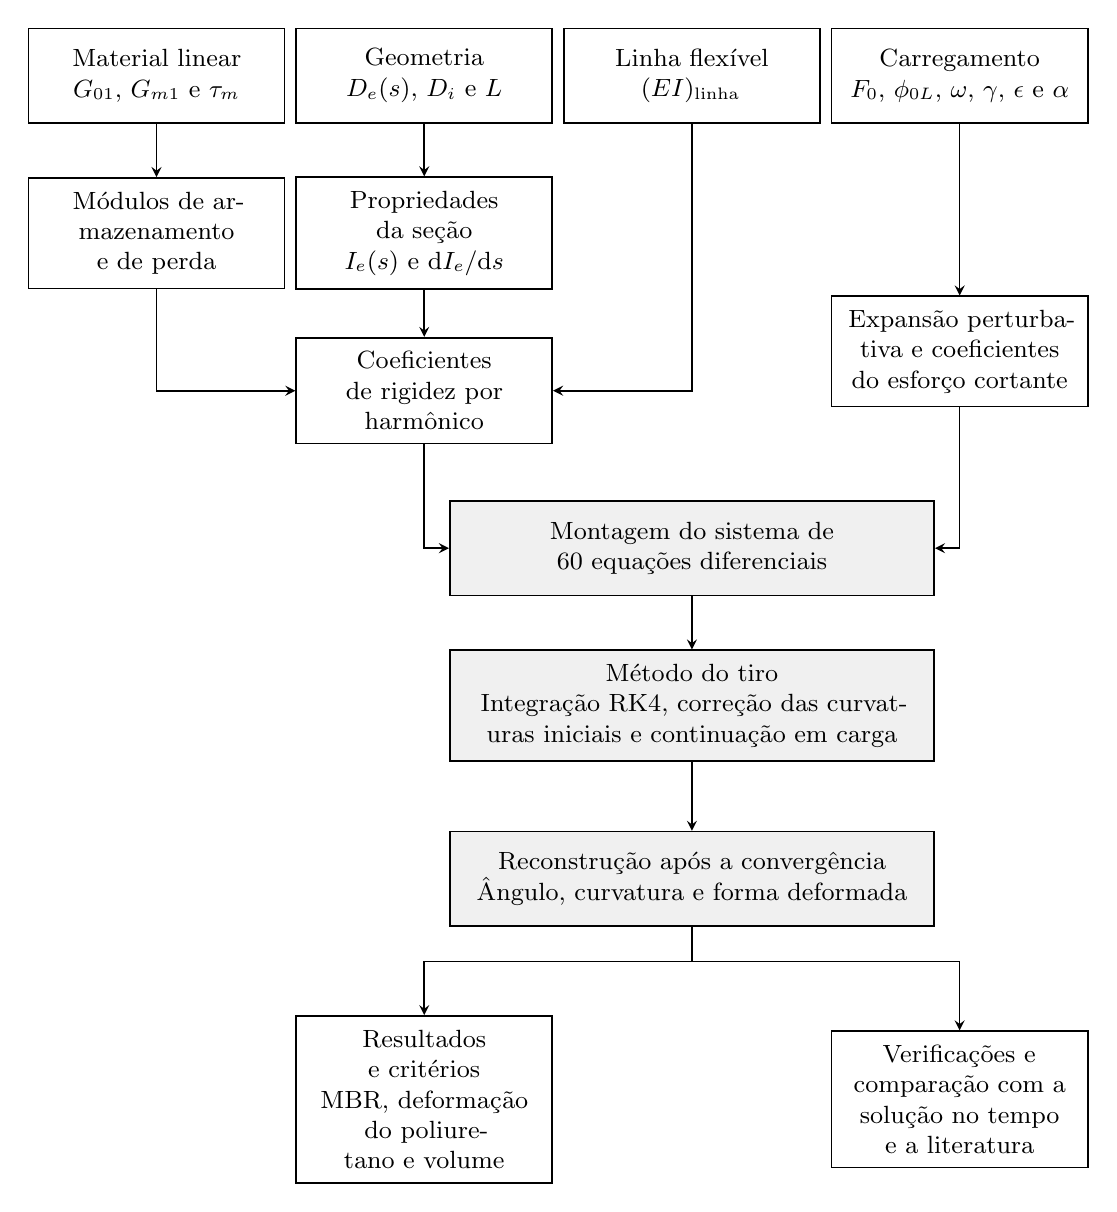
\begin{tikzpicture}[
    processo/.style={draw, line width=0.6pt, fill=white, align=center,
      text width=2.9cm, minimum height=1.2cm, inner sep=5pt,
      font=\small\linespread{1}\selectfont},
    etapa/.style={processo, fill=gray!12, text width=5.8cm},
    fluxo/.style={->, >=stealth, line width=0.6pt}
  ]
    \node[processo] (material) at (-5.1,0)
      {Material linear\\$G_{01}$, $G_{m1}$ e $\tau_m$};
    \node[processo] (geometria) at (-1.7,0)
      {Geometria\\$D_e(s)$, $D_i$ e $L$};
    \node[processo] (linha) at (1.7,0)
      {Linha flexível\\$(EI)_{\mathrm{linha}}$};
    \node[processo] (carga) at (5.1,0)
      {Carregamento\\$F_0$, $\phi_{0L}$, $\omega$, $\gamma$, $\epsilon$ e $\alpha$};
    \node[processo] (modulos) at (-5.1,-2)
      {Módulos de armazenamento e de perda};
    \node[processo] (secao) at (-1.7,-2)
      {Propriedades da seção\\$I_e(s)$ e $\mathrm{d}I_e/\mathrm{d}s$};
    \node[processo] (rigidez) at (-1.7,-4)
      {Coeficientes de rigidez por harmônico};
    \node[processo] (esforcos) at (5.1,-3.5)
      {Expansão perturbativa e coeficientes do esforço cortante};
    \node[etapa] (edos) at (1.7,-6)
      {Montagem do sistema de 60 equações diferenciais};
    \node[etapa] (tiro) at (1.7,-8)
      {Método do tiro\\Integração RK4, correção das curvaturas iniciais e continuação em carga};
    \node[etapa] (resposta) at (1.7,-10.2)
      {Reconstrução após a convergência\\Ângulo, curvatura e forma deformada};
    \node[processo] (criterios) at (-1.7,-13)
      {Resultados e critérios\\MBR, deformação do poliuretano e volume};
    \node[processo] (validacao) at (5.1,-13)
      {Verificações e comparação com a solução no tempo e a literatura};
    \draw[fluxo] (material) -- (modulos);
    \draw[fluxo] (geometria) -- (secao);
    \draw[fluxo] (modulos.south) -- (-5.1,-4) -- (rigidez.west);
    \draw[fluxo] (secao) -- (rigidez);
    \draw[fluxo] (linha.south) -- (1.7,-4) -- (rigidez.east);
    \draw[fluxo] (carga) -- (esforcos);
    \draw[fluxo] (rigidez.south) -- (-1.7,-6) -- (edos.west);
    \draw[fluxo] (esforcos.south) -- (5.1,-6) -- (edos.east);
    \draw[fluxo] (edos) -- (tiro);
    \draw[fluxo] (tiro) -- (resposta);
    \draw[fluxo] (resposta.south) -- (1.7,-11.25) -- (-1.7,-11.25) -- (criterios.north);
    \draw[fluxo] (resposta.south) -- (1.7,-11.25) -- (5.1,-11.25) -- (validacao.north);
  \end{tikzpicture}
  \fonte{Autoria própria}
\end{figure}

A comparação com a literatura deve distinguir os dados publicados em tabelas dos valores
obtidos por leitura de gráficos, sujeitos à precisão dessa leitura. Da mesma forma, parâmetros
ajustados para aproximar o caso de referência precisam ser identificados, pois a concordância
obtida por esse ajuste não constitui, isoladamente, uma validação independente.

As principais grandezas avaliadas são a curvatura da linha, a deformação nas fibras externas
do poliuretano e as posições em que seus máximos ocorrem. O enrijecedor deve proporcionar
uma transição gradual de rigidez sem permitir que a linha exceda sua curvatura admissível.
O raio mínimo de curvatura permitido para a linha, denominado \emph{Minimum Bending Radius}
(MBR), é um dado de projeto. A curvatura admissível correspondente é:

\begin{equation}
\label{eq:mbr}
\kappa_\text{adm} = \frac{1}{\text{MBR}}.
\end{equation}

O critério é atendido quando o maior valor absoluto da curvatura calculada ao longo do
comprimento e do ciclo não ultrapassa $\kappa_\text{adm}$. Para o caso de referência,
adota-se $\text{MBR}=2{,}0\,\mathrm{m}$, conforme \citeonline{Caire2011}.

Para o enrijecedor, avalia-se a deformação por flexão na fibra externa de cada seção.
Considerando a seção circular, a simetria entre tração e compressão e o alongamento axial
desprezado, essa deformação é calculada por:

\begin{equation}
\label{eq:deformacao-maxima}
\varepsilon_\text{ext}(s,t) = \frac{D_e(s)}{2}\,\kappa(s,t),
\end{equation}

em que $s$ é a posição ao longo do conjunto, $t$ representa o tempo no ciclo e $D_e(s)$
é o diâmetro externo do enrijecedor. A deformação máxima é obtida buscando o maior valor
absoluto desse produto apenas no trecho ocupado pelo poliuretano. Como o diâmetro varia,
a posição de maior deformação não precisa coincidir com a de maior curvatura.

Adota-se o limite de deformação de 15\% utilizado no caso de referência de
\citeonline{Caire2011}. Esse valor é um critério do caso estudado, e não
uma propriedade universal de materiais viscoelásticos. A verificação desse limite não
substitui uma avaliação de vida à fadiga, de contato ou de outros modos de falha que não
são calculados pelo modelo.

\section{Premissas Adotadas}
\label{sec:premissas-adotadas}

% Premissas adotadas para o modelo local
O modelo local busca determinar as curvaturas e deformações do conjunto linha flexível-enrijecedor,
considerando o comportamento viscoelástico do poliuretano. Para isso, adotam-se simplificações
que permitem estudar a flexão sem representar todos os detalhes da estrutura real. As premissas
tomam como base a formulação de \citeonline{Caire2011}, com a delimitação
adicional de manter constante a temperatura do material.

% Aproximação de Euler-Bernoulli para a flexão do conjunto linha flexível-enrijecedor
O conjunto é representado pela teoria de vigas de Euler-Bernoulli, desprezando-se a deformação
por cisalhamento para concentrar a análise na deformação por flexão. Essa aproximação tem
apoio nas avaliações discutidas no referencial teórico, em~\ref{sub:deflexao-vigas},
mas deve ser aplicada a geometrias nas quais a contribuição do cisalhamento seja pequena.

% Representação da fixação do conjunto linha flexível-enrijecedor
Na região de topo, acessórios como o \emph{hang-off} sustentam a linha e transferem seus
esforços à estrutura da unidade de produção. Quando o conjunto de fixação possui elevada
rigidez e restringe tanto os deslocamentos quanto as rotações, sua ligação pode ser
representada por um engaste. Neste trabalho, considera-se essa condição para a linha
flexível e o enrijecedor, na mesma extremidade de referência. A presença do acessório, por
si só, não garante essa condição: conexões que permitem rotação ou possuem pontos de fixação
afastados precisam ser representadas de outra forma.

% Justificando o desprezo do alongamento axial.
A linha flexível pode se curvar sem apresentar um aumento significativo de comprimento,
pois possui elevada rigidez axial, ou seja, oferece grande oposição ao alongamento. Por isso, 
considera-se que o comprimento medido ao longo do eixo do conjunto permanece constante durante
a flexão. A mesma aproximação é adotada para o enrijecedor, deixando o cálculo de seu 
alongamento fora do escopo do modelo. Isso não significa retirar a força de tração da análise:
ela continua atuando e influencia a forma assumida pelo conjunto. Também não impede que, ao 
se curvar, as fibras de um lado se alonguem e as do lado oposto se encurtem. O que se despreza
é o aumento do comprimento do eixo, e essa aproximação é adequada quando tal aumento é pequeno
nas condições estudadas.

% Justificando o desprezo da folga radial.
Entre a superfície externa da linha flexível e a superfície interna do enrijecedor pode existir
uma pequena folga. Antes de encostar no enrijecedor, a linha pode se mover dentro desse espaço.
Para simplificar a análise, despreza-se essa folga e considera-se que os dois componentes
acompanham a mesma deflexão. Essa aproximação é adequada quando a folga pouco altera a forma
deformada do conjunto. Não se considera que os materiais estejam colados, e o modelo não
descreve as pressões de contato nem o desgaste entre suas superfícies.

% Justificando a simetria da seção e a escolha do eixo neutro.
Materiais poliméricos podem apresentar respostas diferentes quando tracionados e comprimidos.
Essa diferença é relevante na flexão, pois uma parte da seção trabalha em tração e outra em
compressão, podendo alterar a posição do eixo neutro e a relação entre momento e curvatura
\cite{Caire2011}. Neste trabalho, essa diferença é desprezada: os mesmos parâmetros
são utilizados para representar os dois comportamentos. Trata-se de uma hipótese simplificadora
para estudar os efeitos da viscoelasticidade, e não de uma afirmação de que o poliuretano
responde igualmente à tração e à compressão. Assim, os resultados não incluem os efeitos
dessa assimetria.

% Justificando a escolha do carregamento harmônico.
A força aplicada e o ângulo de topo são representados por funções harmônicas, com valores
médios, amplitudes, frequência e fase relativa definidos. Isso permite estudar como a rapidez
com que a carga se repete influencia a resposta do poliuretano e a energia dissipada a cada
ciclo. É uma condição controlada de análise, que não representa toda a irregularidade do
carregamento real nem garante, por si só, resultados conservadores. Mesmo com uma entrada
harmônica, a resposta do conjunto pode não ser uma senoide pura, devido à não linearidade
geométrica.

O equilíbrio do modelo local é considerado quase-estático: para cada instante, os
esforços são equilibrados sem incluir forças de inércia. As solicitações transmitidas
pela análise global são representadas pela força e pelo ângulo na extremidade do
domínio. Não se acrescentam, nesse trecho local, o peso próprio ou outras ações
distribuídas. Essa simplificação não elimina os efeitos do ambiente na análise global,
nem a dependência temporal e a dissipação de energia do material.

% Justificando a condição isotérmica de referência.
A temperatura também pode alterar a resposta do poliuretano. Além das condições do ambiente,
o próprio carregamento cíclico pode aquecer o material pela dissipação de energia. Neste
trabalho, esses efeitos são desprezados e considera-se uma temperatura constante, correspondente
à utilizada na caracterização do material (24°C). Dessa forma, a análise fica restrita à resposta
mecânica, sem calcular o aquecimento ou a mudança das propriedades com a temperatura.
Essa simplificação não significa que os efeitos térmicos sejam irrelevantes em serviço;
situações com variações importantes de temperatura exigem uma avaliação específica.

Com base nessas considerações, as premissas são sintetizadas a seguir:
\begin{enumerate}
  \item O conjunto é representado pela teoria de vigas de Euler-Bernoulli, desprezando-se
  a deformação por cisalhamento.
  \item A linha flexível e o enrijecedor são considerados engastados na mesma extremidade
  de referência.
  \item O alongamento axial da linha de referência das duas estruturas é desprezado,
  mantendo-se a força de tração no equilíbrio.
  \item O espaçamento radial entre a linha flexível e o enrijecedor é desprezado,
  adotando-se a mesma deflexão para ambos.
  \item As respostas constitutivas em tração e compressão são consideradas simétricas,
  preservando-se o comportamento viscoelástico do poliuretano.
  \item A força aplicada e o ângulo de topo são representados por funções harmônicas.
  \item O equilíbrio local é quase-estático, desprezando-se forças de inércia,
  peso próprio e outras ações distribuídas no domínio analisado.
  \item Os parâmetros constitutivos correspondem a uma condição de temperatura de referência,
  sem considerar variações térmicas ou acoplamento termomecânico.
\end{enumerate}

% Ajustes necessarios para o material
\section{Caracterização do Material}
\label{sec:caracterizacao-do-material}

A caracterização tem como finalidade obter os parâmetros que descrevem a redução da tensão
ao longo do tempo nos ensaios de relaxação. Esses parâmetros são utilizados
na representação viscoelástica do poliuretano e, posteriormente, no cálculo da resposta
estrutural. O procedimento parte das curvas de relaxação, ajusta seus termos exponenciais e
identifica a função de relaxação utilizada no modelo linear. A relação entre dados experimentais, funções de relaxação e
parâmetros constitutivos também constitui a base da caracterização discutida por
\citeonline{Pagliosa2004}.

\subsection{Dados Experimentais}
\label{sec:dados-experimentais}

Neste trabalho, não foi realizada uma campanha experimental própria. Os dados de entrada foram
obtidos por digitalização dos gráficos dos ensaios de relaxação publicados por
\citeonline{Caire2011}. Na campanha descrita na tese, foram preparados 50 corpos de
prova de poliuretano extraídos de um enrijecedor real, destinados aos ensaios de tração e
relaxação. Os ensaios de relaxação considerados nesta identificação correspondem a seis níveis
de deformação: 2,5\%, 5\%, 7,5\%, 10\%, 20\% e 30\%, mantidos por aproximadamente quatro horas,
em temperatura laboratorial de cerca de $24\,^{\circ}\mathrm{C}$. O total de corpos de prova
da campanha não corresponde, portanto, ao número de curvas utilizadas no ajuste.

Os pares de tempo e tensão digitalizados são organizados em seis arquivos CSV, um para cada
nível de deformação. O programa lê o tempo em segundos e a tensão em MPa, utilizando a coluna
de valores de ensaio, e não a coluna de ajuste presente nesses arquivos. Por se tratar de
digitalização, esses valores não equivalem aos registros
originais da máquina de ensaio e estão sujeitos à resolução dos gráficos e à precisão da
leitura.

Antes do ajuste, o programa remove registros sem valores numéricos válidos, ordena os dados
pelo tempo e, quando há tempos repetidos, utiliza a média das tensões correspondentes.
Na configuração adotada, são utilizados os pontos com $t\geq1\,\mathrm{s}$, até o último
instante disponível em cada arquivo. Dessa forma, o ajuste não inclui diretamente o instante
inicial nem a etapa de aplicação da deformação. A identificação se limita à parte da curva
disponível nos dados, e não constitui uma avaliação da dispersão entre corpos de prova.

\subsection{Ajuste dos Termos da Série de Prony}
\label{sec:ajuste-prony}

Cada curva de tensão é representada por um termo constante e quatro termos exponenciais:

\begin{equation}
  \label{eq:ajuste-tensao-prony}
  \widehat{\sigma}_i(t)=\sigma_{0i}
  +\sum_{m=1}^{4}\sigma_{mi}\exp\left(-\frac{t}{\tau_m}\right),
\end{equation}

em que $i$ identifica o nível de deformação, $\widehat{\sigma}_i(t)$ é a tensão ajustada,
$\sigma_{0i}$ é o valor de longo prazo previsto pelo ajuste e $\sigma_{mi}$ são as
contribuições dos termos associados aos tempos de relaxação $\tau_m$. Os coeficientes de
tensão são próprios de cada curva, enquanto os quatro tempos são comuns às seis curvas.
Esse número de termos acompanha a representação utilizada no caso de referência de
\citeonline{Caire2011}.

A identificação é realizada em duas etapas combinadas. O método dos mínimos quadrados busca
os parâmetros que reduzem a soma dos quadrados das diferenças entre a curva calculada e
os dados de relaxação. Para uma estimativa dos tempos,
calculam-se os cinco coeficientes de cada curva por mínimos quadrados, impondo valores
não negativos. Em seguida, os tempos são atualizados para reduzir o erro conjunto das
seis curvas. Esse processo utiliza as rotinas \texttt{lsq\_linear} e
\texttt{least\_squares} da biblioteca SciPy. Os tempos são parametrizados por incrementos
positivos, mantendo-se $\tau_1<\tau_2<\tau_3<\tau_4$ durante a busca.

Para evitar que uma curva domine o ajuste apenas por apresentar tensões maiores ou mais
pontos, seus resíduos são divididos pela amplitude de variação da tensão e pela raiz
quadrada do número de pontos. Para as curvas utilizadas, a função objetivo é:

\begin{equation}
  \label{eq:objetivo-ajuste-global}
  J=\sum_{i=1}^{6}\frac{1}{n_i(\Delta\sigma_i)^2}
  \sum_{j=1}^{n_i}
  \left[\widehat{\sigma}_i(t_{ij})-\sigma_i(t_{ij})\right]^2,
\end{equation}

em que $n_i$ é o número de pontos da curva $i$, $t_{ij}$ é o tempo do ponto $j$ e
$\Delta\sigma_i$ é a diferença entre a maior e a menor tensão dessa curva. A ponderação
equilibra a participação das curvas sem alterar as unidades dos coeficientes finais.

Na configuração do programa, as estimativas iniciais dos tempos são 1, 10, 100 e
1000 segundos. Sua atualização utiliza o algoritmo de região de confiança
\emph{Trust Region Reflective}, identificado pela opção \texttt{trf} da SciPy
\cite{SciPyLeastSquares}. A ideia é prever como uma pequena mudança nos parâmetros altera
o erro, utilizando uma aproximação local da função objetivo. Em vez de permitir qualquer
mudança de uma só vez, o algoritmo limita o passo a uma região na qual essa aproximação
é considerada confiável.

Após testar os novos parâmetros, compara-se a redução de erro obtida com a prevista.
Quando há boa concordância, a região pode ser ampliada; quando a previsão é inadequada,
ela pode ser reduzida para que o próximo passo seja mais cauteloso. O procedimento evita
depender de grandes mudanças baseadas em uma aproximação válida apenas nas proximidades
da estimativa atual. A variante reflexiva também permite lidar com limites impostos aos
parâmetros. Na busca dos tempos deste trabalho, porém, a positividade e a ordenação são
garantidas pela parametrização por incrementos positivos.

São utilizadas tolerâncias de $10^{-12}$ para os critérios de parada e um limite de
5000 avaliações da função objetivo. Os critérios acompanham a mudança do erro, a mudança
dos parâmetros e o gradiente, que indica a tendência local de variação do erro. A convergência
numérica não garante que os parâmetros sejam únicos ou que o erro da digitalização tenha
sido eliminado. Após a identificação dos tempos, os coeficientes de tensão são recalculados
para cada curva.

\subsection{Identificação das Funções de Relaxação}
\label{sec:identificacao-funcoes-relaxacao}

O ajuste anterior descreve cada curva de relaxação separadamente. Para reunir essas curvas,
é necessário representar como a tensão muda tanto com o tempo quanto com o nível de
deformação. Em um material viscoelástico linear, dobrar a deformação de um ensaio ideal de
relaxação dobra a tensão em todos os instantes. Quando essa proporcionalidade não ocorre,
uma única função linear não descreve toda a família de curvas.

O princípio da superposição modificado (PSM), apresentado na
Subseção~\ref{sub:psm}, fornece uma forma de representar a memória
do material sem exigir essa proporcionalidade. Na representação integral de
\citeonline{PipkinRogers1968}, a resposta depende das deformações aplicadas anteriormente,
e essa dependência pode ser não linear. Para a identificação a partir dos ensaios de
relaxação, adota-se a aproximação polinomial em que cada potência da deformação possui sua
própria função de relaxação. Assim, não se exige que todas as curvas sejam múltiplos de
uma mesma curva. A tensão ajustada é escrita como:

\begin{equation}
  \label{eq:psm-constitutivo}
  \widehat{\sigma}(t,\varepsilon)
  =\sum_{k=1}^{4}G_k(t)\varepsilon^k,
\end{equation}

com

\begin{equation}
  \label{eq:psm-relaxacao}
  G_k(t)=G_{0k}
  +\sum_{m=1}^{4}G_{mk}\exp\left(-\frac{t}{\tau_m}\right).
\end{equation}

Nessa representação, $k$ identifica a potência da deformação, $m$ identifica o termo de
relaxação e $G_{0k}$ corresponde ao termo de longo prazo da função $G_k(t)$. A
Equação~\eqref{eq:psm-constitutivo} descreve os ensaios de relaxação; para um carregamento
que varia no tempo, é necessário considerar o histórico de deformação por meio da relação
constitutiva integral, e não apenas substituir a deformação instantânea nesse polinômio.

Substituindo a Equação~\eqref{eq:psm-relaxacao} na
Equação~\eqref{eq:psm-constitutivo}, os coeficientes de tensão de cada curva se relacionam
aos coeficientes do material por:

\begin{equation}
  \label{eq:regressao-coeficientes-material}
  \sigma_{mi}\approx\sum_{k=1}^{4}G_{mk}\varepsilon_i^k,
  \qquad m=0,1,2,3,4.
\end{equation}

Para cada valor de $m$, ajusta-se um polinômio sem termo independente aos seis níveis de
deformação. Os quatro coeficientes são obtidos por mínimos quadrados, utilizando
\texttt{numpy.linalg.lstsq}. O resultado é uma matriz com cinco linhas, correspondentes
ao termo de longo prazo e aos quatro termos exponenciais, e quatro colunas, correspondentes
às funções $G_1$, $G_2$, $G_3$ e $G_4$.

Para melhorar o comportamento numérico dessa regressão, o programa utiliza temporariamente
as deformações divididas por 0,30 e converte os coeficientes de volta à escala original após
o ajuste. Essa mudança de escala não altera os níveis físicos de deformação. Diferentemente
dos coeficientes de tensão da primeira etapa, os coeficientes $G_{mk}$ não são restringidos
a valores positivos nessa regressão.

\subsection{Parâmetros Utilizados no Modelo Linear}
\label{sec:parametros-material-linear}

A identificação polinomial permite representar a variação das curvas com o nível de
deformação, mas a solução estrutural desenvolvida nesta etapa do trabalho utiliza apenas
a parcela linear, associada a $G_1(t)$. Assim:

\begin{equation}
  \label{eq:relaxacao-material-linear}
  G_1(t)=G_{01}
  +\sum_{m=1}^{4}G_{m1}\exp\left(-\frac{t}{\tau_m}\right).
\end{equation}

No programa de solução, $G_{01}$ é utilizado como módulo de longo prazo, $G_{m1}$ como
contribuições de relaxação e $\tau_m$ como tempos característicos, que correspondem a $G_{\infty}$, $G_m$ e $\tau_m$
da série de Prony da Equação~\eqref{eq:prony-relaxacao}. Embora se utilize a letra
$G$, nesta identificação a função relaciona tensão e deformação longitudinais nos ensaios
de tração, não sendo identificada como módulo de cisalhamento.

Para um ensaio ideal de relaxação no modelo linear, a tensão é dada por
$\sigma(t)=G_1(t)\varepsilon$. A utilização somente de $G_1$ elimina os termos de segunda,
terceira e quarta potências da deformação na solução estrutural. Isso não significa que
todas as curvas utilizadas na identificação, inclusive as de maior deformação, sejam
lineares. O bom ajuste da representação polinomial completa também não demonstra, por
si só, que a parcela linear seja adequada em toda a faixa de 2,5\% a 30\%.

Para o modelo linear de Maxwell generalizado, o programa verifica
tempos positivos e contribuições de relaxação não negativas, além da consistência dos
limites inicial e de longo prazo. Os módulos de armazenamento e de perda são calculados
a partir desses parâmetros, conforme as Equações~\eqref{eq:modulo-armazenamento} e
\eqref{eq:modulo-perda}.

Mantêm-se separados dois conjuntos de parâmetros: os publicados na Tabela 2.4 de
\citeonline{Caire2011} e os obtidos pela identificação deste trabalho. A escolha do conjunto
é indicada em cada análise. Dessa forma, diferenças decorrentes da identificação do material
não são confundidas com diferenças da implementação da solução estrutural.

\subsection{Avaliação do Ajuste}
\label{sec:avaliacao-ajuste-material}

A qualidade do ajuste é avaliada comparando as tensões calculadas e digitalizadas ao longo
do tempo, com atenção tanto à parte inicial disponível quanto à parte final de cada curva.
Além dos gráficos, o programa calcula a raiz do erro quadrático médio (RMSE), o erro absoluto
médio (MAE) e o coeficiente de determinação ($R^2$). Para uma curva com $n$ pontos:

\begin{align}
  \mathrm{RMSE}
  &=\sqrt{\frac{1}{n}\sum_{j=1}^{n}
  \left(\widehat{\sigma}_j-\sigma_j\right)^2},
  \label{eq:rmse-ajuste-material}\\
  \mathrm{MAE}
  &=\frac{1}{n}\sum_{j=1}^{n}
  \left|\widehat{\sigma}_j-\sigma_j\right|,
  \label{eq:mae-ajuste-material}\\
  R^2
  &=1-\frac{\sum_{j=1}^{n}
  \left(\widehat{\sigma}_j-\sigma_j\right)^2}
  {\sum_{j=1}^{n}\left(\sigma_j-\overline{\sigma}\right)^2},
  \label{eq:r2-ajuste-material}
\end{align}

em que $\sigma_j$ é a tensão digitalizada, $\widehat{\sigma}_j$ é a tensão ajustada e
$\overline{\sigma}$ é a média das tensões da curva. RMSE e MAE são apresentados em MPa,
enquanto $R^2$ é adimensional. O mesmo conjunto de indicadores é empregado para avaliar
a regressão dos coeficientes de tensão em função da deformação.

Esses indicadores avaliam a concordância com os dados utilizados no ajuste, não uma validação
experimental independente. Também são examinadas a reconstrução das seis curvas pelo
polinômio completo e a comparação dos parâmetros com os valores de referência. Diferenças
podem resultar da digitalização, da ponderação das curvas e do procedimento de otimização.
Por isso, uma pequena diferença entre curvas não implica, necessariamente, igualdade entre
todos os tempos e coeficientes identificados.

Por fim, os tempos, os coeficientes, as curvas reconstruídas e os indicadores são exportados
em arquivos CSV e gráficos. Esses resultados permitem conferir a identificação antes de
selecionar os parâmetros que serão utilizados na análise estrutural.

% Sistemas de Equações
\section{Equacionamento do Sistema Linha Flexível-Enrijecedor}
\label{sec:equacionamento-do-sistema}

\subsection{Caracterização do Sistema}
\label{sec:caracterizacao-sistema}

A caracterização do sistema reúne a geometria do enrijecedor, a rigidez flexional da linha
e os parâmetros do carregamento, conforme o bloco de entrada da
Figura~\ref{fig:fluxo-metodologia-linear}. Enquanto a caracterização do material descreve
como o poliuretano responde ao longo do tempo, essas informações definem onde ele atua
e quais solicitações são aplicadas ao conjunto.

Utiliza-se a coordenada $s$ medida ao longo do eixo do conjunto, com origem no engaste e
extremidade em $s=L$. O domínio inclui o trecho envolvido pelo enrijecedor e um trecho
adicional da linha flexível. Essa distinção é importante: fora do enrijecedor, a resistência
à flexão é fornecida apenas pela linha.

O perfil adotado possui um trecho cilíndrico, com comprimento $L_{\mathrm{cil}}$ e diâmetro
externo $D_b$, seguido de um trecho cônico, com comprimento $L_{\mathrm{con}}$. O diâmetro
interno $D_i$ é constante. Ao final do cone, o diâmetro externo do perfil idealizado se
iguala ao interno, encerrando a contribuição do poliuretano. Definindo
$L_e=L_{\mathrm{cil}}+L_{\mathrm{con}}$, obtém-se o comprimento ocupado pelo enrijecedor.

A Figura~\ref{fig:geometria-souza} apresenta um esquema com os comprimentos e diâmetros
principais, reproduzido de \citeonline{Souza2008}. Na notação da figura,
$L_1$, $L_2$ e $L_{\mathrm{BS}}$ correspondem, respectivamente, a
$L_{\mathrm{cil}}$, $L_{\mathrm{con}}$ e $L_e$, enquanto $D_1$ corresponde a $D_b$.
O símbolo $d_1$ indica o diâmetro externo da linha, não o diâmetro interno $D_i$ do furo
do enrijecedor. A figura auxilia a leitura da geometria, mas o perfil equivalente adotado
no cálculo é definido pela Equação~\eqref{eq:perfil-enrijecedor-metodologia}.

\begin{figure}[!htbp]
  \centering
  \caption{Geometria simplificada do conjunto linha flexível-enrijecedor e suas dimensões principais.}
  \label{fig:geometria-souza}
  \includegraphics[width=0.9\textwidth]{pics/souza2008-geometria.png}
  \fonte{\citeonline{Souza2008}.}
\end{figure}

Com a notação deste trabalho, o diâmetro externo do perfil é escrito como:

\begin{equation}
  \label{eq:perfil-enrijecedor-metodologia}
  D_e(s)=
  \begin{cases}
    D_b, & 0\leq s\leq L_{\mathrm{cil}},\\[1ex]
    D_b-\displaystyle\frac{D_b-D_i}{L_{\mathrm{con}}}
    \left(s-L_{\mathrm{cil}}\right),
      & L_{\mathrm{cil}}<s<L_e,\\[1ex]
    D_i, & L_e\leq s\leq L.
  \end{cases}
\end{equation}

No último trecho, $D_e=D_i$ é apenas uma forma de representar a ausência de poliuretano
no cálculo; não corresponde ao diâmetro externo da linha flexível.

Para cada posição, a área de poliuretano e o momento de inércia da seção anular são:

\begin{align}
  A_e(s)&=\frac{\pi}{4}\left[D_e(s)^2-D_i^2\right],
    \label{eq:area-enrijecedor-metodologia}\\
  I_e(s)&=\frac{\pi}{64}\left[D_e(s)^4-D_i^4\right].
    \label{eq:inercia-enrijecedor-metodologia}
\end{align}

O momento de inércia diminui ao longo do cone, reduzindo gradualmente a contribuição do
enrijecedor à rigidez do conjunto. Como depende da quarta potência dos diâmetros, pequenas
mudanças no perfil podem produzir diferenças relevantes na resposta.

O programa obtém $D_e(s)$ por interpolação linear entre os pontos que definem o perfil
e calcula a derivada de $I_e(s)$ em cada trecho por:

\begin{equation}
  \label{eq:derivada-inercia-metodologia}
  \frac{\mathrm{d}I_e}{\mathrm{d}s}
  =\frac{\pi}{16}D_e(s)^3\frac{\mathrm{d}D_e}{\mathrm{d}s}.
\end{equation}

Nas junções, a inclinação do perfil muda. Essas posições são identificadas para que a
integração numérica trate os trechos separadamente, evitando atravessar uma mudança de
expressão como se o perfil tivesse a mesma inclinação em todo o domínio.

No caso de referência, utilizam-se um trecho cilíndrico de 0,20 m, um trecho cônico de
1,50 m e mais 1,30 m de linha, totalizando $L=3{,}00\,\mathrm{m}$. O diâmetro externo
na base é $D_b=0{,}70\,\mathrm{m}$, seguindo a configuração da Figura 4.3 de
\citeonline{Caire2011}. O diâmetro interno adotado no código é $D_i=0{,}34\,\mathrm{m}$,
registrado na implementação como parâmetro calibrado para aproximar resultados de
referência. Portanto, esse valor não deve ser apresentado como uma dimensão diretamente
fornecida pela tese, nem a comparação utilizada na calibração como uma verificação
independente.

A linha flexível é representada por uma rigidez flexional equivalente constante,
$(EI)_{\mathrm{linha}}$, sem modelar separadamente suas camadas. No caso de referência,
adota-se $(EI)_{\mathrm{linha}}=50\,000\,\mathrm{N\,m^2}$. Essa rigidez é somada à
contribuição do poliuretano na montagem dos coeficientes do sistema, enquanto a geometria
do enrijecedor determina a variação dessa contribuição ao longo de $s$.

O carregamento é definido pela força e pelo ângulo prescritos na extremidade $s=L$:

\begin{align}
  F(t)&=F_0\left[1+\epsilon\sin(\omega t)\right],
    \label{eq:forca-harmonica-metodologia}\\
  \phi_L(t)&=\phi_{0L}
    \left[1+\alpha\sin(\omega t+\gamma)\right].
    \label{eq:angulo-harmonico-metodologia}
\end{align}

Os parâmetros $F_0$ e $\phi_{0L}$ são os valores médios, $\epsilon$ e $\alpha$ controlam
as amplitudes relativas e $\gamma$ define a diferença de fase. A frequência angular é
$\omega=2\pi f$. Aqui, $\epsilon$ representa a amplitude relativa da força, não a
deformação do material usada na caracterização.

A diferença de fase permite que os máximos de força e de ângulo ocorram em instantes
distintos, o que influencia a resposta do conjunto. Na configuração de referência do
código, são utilizados $F_0=660\,\mathrm{kN}$, $\phi_{0L}=18^\circ$,
$\gamma=15{,}47^\circ$, $f=0{,}04\,\mathrm{Hz}$, $\epsilon=0{,}45$ e
$\alpha=0{,}27$. A partir dessas entradas, são montados os esforços e as equações
diferenciais que serão discutidos a seguir.

\subsection{Relações Trigonométricas}
\label{sec:relacoes-trigonometricas}

A forma deformada do conjunto pode ser descrita a partir de pequenos trechos de seu
eixo. A Figura~\ref{fig:elemento-infinitesimal-caire}, reproduzida de
\citeonline{Caire2011}, apresenta um elemento de comprimento $\mathrm{d}s$,
suas projeções $\mathrm{d}x$ e $\mathrm{d}y$ e os esforços internos atuantes nas
seções. O eixo $X$ aponta para baixo, a partir do engaste, e o eixo $Y$ para a
esquerda, conforme a convenção da figura. O ângulo $\phi(s,t)$ é medido entre a
tangente à linha e o eixo $X$.

\begin{figure}[!htbp]
  \centering
  \caption{Elemento infinitesimal do conjunto, projeções geométricas e esforços internos.}
  \label{fig:elemento-infinitesimal-caire}
  \includegraphics[width=0.55\textwidth]{pics/caire2011-elemento-infinitesimal.png}
  \fonte{\citeonline{Caire2011}.}
\end{figure}

Para um instante fixo, as projeções do elemento são
$\mathrm{d}x=\cos\phi\,\mathrm{d}s$ e
$\mathrm{d}y=\sin\phi\,\mathrm{d}s$. Dividindo pelo comprimento do elemento e tomando
o limite diferencial, obtêm-se:

\begin{align}
  \frac{\partial x(s,t)}{\partial s}&=\cos\phi(s,t),
    \label{eq:geometria-x-metodologia}\\
  \frac{\partial y(s,t)}{\partial s}&=\sin\phi(s,t).
    \label{eq:geometria-y-metodologia}
\end{align}

Como o comprimento do eixo é considerado constante, $s$ identifica a mesma posição
material durante a flexão. As relações anteriores também mostram que as projeções
podem mudar sem que o comprimento do elemento se altere.

A curvatura mede quanto a direção da tangente muda por unidade de comprimento.
Se o elemento é aproximado localmente por um arco de raio $\rho$, o módulo da
variação angular é $|\mathrm{d}\phi|=\mathrm{d}s/\rho$. Assim:

\begin{equation}
  \kappa(s,t)=\frac{\partial\phi(s,t)}{\partial s},
  \label{eq:geometria-curvatura-metodologia}
\end{equation}

com $|\kappa|=1/\rho$ para o raio geométrico positivo. O sinal da curvatura indica
o sentido da flexão.

Essas relações permitem obter as coordenadas deformadas integrando o ângulo ao
longo de $s$. Não se utiliza aqui a aproximação $\sin\phi\approx\phi$: o modelo
admite rotações finitas, ainda que as deformações do material sejam tratadas de
forma simplificada. A integração geométrica é realizada após a solução dos
campos de ângulo e curvatura, conforme a Seção~\ref{sec:reconstrucao-da-resposta}.

\subsection{Equilíbrio de Forças e Momentos}
\label{sec:sistema-equacoes}

O diagrama de corpo livre da Figura~\ref{fig:dcl-souza} auxilia a interpretação do
equilíbrio do conjunto: a linha é engastada em $s=0$, recebe a força $F$ na extremidade
$s=L$ e apresenta rigidez flexional variável ao longo do trecho envolvido pelo
enrijecedor. O detalhe de um elemento da linha indica os esforços internos que
participam do equilíbrio. Essa representação, originalmente atribuída a Boef e Out
(1990), foi reproduzida por \citeonline{Souza2008}.

\begin{figure}[!htbp]
  \centering
  \caption{Diagrama de forças e equilíbrio de um elemento do conjunto linha flexível-enrijecedor.}
  \label{fig:dcl-souza}
  \includegraphics[width=0.65\textwidth]{pics/souza2008-dcl.png}
  \fonte{Boef e Out (1990), reproduzido em \citeonline{Souza2008}.}
\end{figure}

Mantém-se na figura a notação da fonte original. O ângulo da linha, indicado por
$\theta$, é representado neste trabalho por $\phi$, e o raio de curvatura $\rho$
se relaciona à curvatura por $\kappa=1/\rho$. O ângulo $\alpha$ indicado no diagrama
entre a força e a tangente à linha não deve ser confundido com o parâmetro $\alpha$
de amplitude relativa do carregamento harmônico. O esquema serve de apoio ao equilíbrio;
a resposta dependente do tempo é incorporada por meio da descrição viscoelástica
do material.

O equilíbrio é aplicado para cada instante de tempo, sem forças distribuídas ou
de inércia no domínio local. Denotando por $\theta_F(t)$ a direção da força em
relação ao eixo $X$, a formulação geral permite escrever
$\theta_F(t)=\phi_L(t)+\beta$, em que $\beta$ é o ângulo entre a força e a tangente
na extremidade. No modelo implementado, adota-se $\beta=0$, de modo que a força
acompanha a direção definida pelo ângulo de contorno. O ângulo relativo entre a
força e uma seção genérica é:

\begin{equation}
  \theta(s,t)=\theta_F(t)-\phi(s,t).
  \label{eq:angulo-relativo-equilibrio}
\end{equation}

Projetando a força nas direções tangente e normal à seção, obtêm-se os esforços
de tração $T$ e cortante $V$. Com a convenção de sinais adotada por
\citeonline{Caire2011}, escreve-se:

\begin{align}
  T(s,t)&=F(t)\cos\theta(s,t),
    \label{eq:tracao-equilibrio}\\
  V(s,t)&=-F(t)\sin\theta(s,t).
    \label{eq:cortante-equilibrio}
\end{align}

O sinal negativo do cortante decorre da orientação dos esforços na
Figura~\ref{fig:elemento-infinitesimal-caire}. Mesmo com força constante ao longo
do domínio em um dado instante, essas duas projeções variam porque a direção
da tangente muda de uma seção para outra.

Utilizando $\partial\phi/\partial s=\kappa$, as relações diferenciais de
equilíbrio das forças e do momento são:

\begin{align}
  \frac{\partial T}{\partial s}&=-\kappa V,
    \label{eq:equilibrio-diferencial-tracao}\\
  \frac{\partial V}{\partial s}&=\kappa T,
    \label{eq:equilibrio-diferencial-cortante}\\
  \frac{\partial M}{\partial s}&=V.
    \label{eq:equilibrio-diferencial-momento}
\end{align}

As duas primeiras expressões acompanham a mudança das direções locais de
projeção. A terceira relaciona a variação do momento fletor ao esforço cortante
e é utilizada diretamente na obtenção das equações de governo.

O momento em uma seção também pode ser expresso pelo braço da força até
a extremidade do domínio:

\begin{equation}
  \begin{aligned}
    M(s,t)=M(L,t)+F(t)\bigl\{&
      \sin\theta_F(t)\,[x(L,t)-x(s,t)]\\
      &-\cos\theta_F(t)\,[y(L,t)-y(s,t)]\bigr\}.
  \end{aligned}
  \label{eq:momento-braco-forca}
\end{equation}

Mantém-se nessa expressão o momento terminal $M(L,t)$, pois a extremidade do
domínio local é uma seção da linha, e não necessariamente sua terminação física.
Quando esse momento é nulo, recupera-se a expressão baseada somente no braço
da força. Sua derivada em relação a $s$ fornece, em ambos os casos,
a Equação~\eqref{eq:cortante-equilibrio}.

Para relacionar o equilíbrio ao material, considera-se a deformação longitudinal
de uma fibra situada à distância $\eta$ do eixo neutro:

\begin{equation}
  \varepsilon(\eta,s,t)=\eta\,\kappa(s,t),
  \label{eq:deformacao-fibra-metodologia}
\end{equation}

com a orientação de $\eta$ escolhida de acordo com o sinal do momento. A
deformação varia linearmente na seção, mas a tensão do poliuretano também
depende do histórico dessa deformação. Sob as hipóteses de seção concêntrica
e resposta simétrica em tração e compressão, o eixo neutro de flexão passa
pelo centro da seção.

O momento total é a soma das contribuições da linha e do enrijecedor:

\begin{equation}
  M(s,t)=M_{\mathrm{linha}}(s,t)+M_e(s,t)
  =\int_{A_{\mathrm{linha}}}\sigma_{\mathrm{linha}}\eta\,\mathrm{d}A
   +\int_{A_e}\sigma_e\eta\,\mathrm{d}A.
  \label{eq:momento-soma-componentes}
\end{equation}

Na representação equivalente adotada, a primeira parcela é descrita por
$(EI)_{\mathrm{linha}}\kappa$. A segunda é obtida pela relação constitutiva
viscoelástica linear, desenvolvida a seguir. A tração permanece no equilíbrio
do conjunto, embora seu alongamento axial não seja calculado.

\subsection{Condições de Contorno}
\label{sec:condicoes-contorno}

O engaste fixa a origem e a direção inicial da linha. Na extremidade do domínio,
prescreve-se o ângulo fornecido pelo carregamento. Assim:

\begin{equation}
  x(0,t)=0,\qquad y(0,t)=0,\qquad
  \phi(0,t)=0,\qquad \phi(L,t)=\phi_L(t).
  \label{eq:contorno-geometrico-metodologia}
\end{equation}

As duas primeiras condições definem a posição do conjunto, enquanto as duas
últimas delimitam a solução de ângulo e curvatura. Não se impõe adicionalmente
$M(L,t)=0$: no domínio finito utilizado pelo programa, o contorno é definido
pelo ângulo terminal. O momento nessa seção é obtido da solução. As condições
dos coeficientes harmônicos correspondentes serão apresentadas após sua definição.

\section{Equações de Governo para Viscoelasticidade Linear}
\label{sec:implementando-viscoelasticidade}

As equações de governo reúnem as relações geométricas, o equilíbrio e a resposta
do material. A formulação apresentada nesta seção segue o desenvolvimento da
seção 3.4 de \citeonline{Caire2011}, utilizando a função longitudinal $G_1(t)$
identificada na Seção~\ref{sec:caracterizacao-do-material}. Apresenta-se primeiro
a relação no domínio do tempo, para explicitar a memória do material, e depois
a formulação harmônica em regime permanente utilizada na solução principal.

\subsection{Formulação no Domínio do Tempo}
\label{sec:governo-linear-tempo}

Para o material inicialmente sem deformação, a tensão longitudinal pode ser
escrita em função do histórico de deformação:

\begin{equation}
  \sigma_e(\eta,s,t)=G_1(0)\varepsilon(\eta,s,t)
  +\int_0^t \dot G_1(t-\tau)\,
    \varepsilon(\eta,s,\tau)\,\mathrm{d}\tau.
  \label{eq:constitutiva-linear-historico}
\end{equation}

O ponto em $\dot G_1$ indica a derivada em relação ao tempo de relaxação,
$\dot G_1(u)=\mathrm{d}G_1(u)/\mathrm{d}u$, e $\tau$ representa um instante
anterior. A primeira parcela contém o módulo instantâneo $G_1(0)$; a integral
considera a mudança dessa contribuição com o tempo. Para um ensaio ideal de
relaxação, a deformação aplicada permanece constante e essa expressão se reduz
a $\sigma_e(t)=G_1(t)\varepsilon$. Para um histórico variável, entretanto, a
integral não pode ser substituída por essa multiplicação.

Substituindo a Equação~\eqref{eq:deformacao-fibra-metodologia} na relação
constitutiva e integrando as tensões na seção, obtém-se:

\begin{equation}
  \begin{aligned}
    M(s,t)={}&\bigl[(EI)_{\mathrm{linha}}+I_e(s)G_1(0)\bigr]\kappa(s,t)\\
      &+I_e(s)\int_0^t
        \dot G_1(t-\tau)\kappa(s,\tau)\,\mathrm{d}\tau.
  \end{aligned}
  \label{eq:momento-curvatura-linear-tempo}
\end{equation}

O momento de inércia $I_e(s)$ aparece porque
$\int_{A_e}\eta^2\,\mathrm{d}A=I_e(s)$. A contribuição elástica da linha
responde à curvatura atual, enquanto o poliuretano também conserva a influência
das curvaturas anteriores.

Diferenciando o momento em relação a $s$ e utilizando
$\partial M/\partial s=V=-F(t)\sin\theta(s,t)$, chega-se à equação de governo:

\begin{equation}
  \begin{aligned}
    \frac{\partial\kappa(s,t)}{\partial s}
    =-\frac{1}{(EI)_{\mathrm{linha}}+G_1(0)I_e(s)}
    \Biggl\{&F(t)\sin\theta(s,t)\\
      &+I_e(s)\int_0^t \dot G_1(t-\tau)
        \frac{\partial\kappa(s,\tau)}{\partial s}\,\mathrm{d}\tau\\
      &+\frac{\mathrm{d}I_e(s)}{\mathrm{d}s}
        \left[G_1(0)\kappa(s,t)
        +\int_0^t\dot G_1(t-\tau)\kappa(s,\tau)\,\mathrm{d}\tau\right]
    \Biggr\}.
  \end{aligned}
  \label{eq:governo-curvatura-linear-tempo}
\end{equation}

Essa equação mostra três influências na variação espacial da curvatura:
a força aplicada, a memória do poliuretano e a mudança da geometria da seção.
Juntamente com as Equações~\eqref{eq:geometria-x-metodologia},
\eqref{eq:geometria-y-metodologia} e
\eqref{eq:geometria-curvatura-metodologia}, forma o sistema de quatro equações
integro-diferenciais no domínio do tempo, sujeito às condições da
Equação~\eqref{eq:contorno-geometrico-metodologia}.

No instante inicial idealizado, as integrais se anulam e o sistema apresenta a
rigidez instantânea $(EI)_{\mathrm{linha}}+G_1(0)I_e(s)$. Já durante a evolução,
o cálculo requer o histórico de curvatura. A solução harmônica a seguir evita
acompanhar esse histórico explicitamente quando o interesse é a resposta
periódica após o desaparecimento dos transientes.

\subsection{Resposta Harmônica e Aplicação do Método da Perturbação}
\label{sec:aplicacao-metodo-perturbacao}

O carregamento é definido pelas
Equações~\eqref{eq:forca-harmonica-metodologia} e
\eqref{eq:angulo-harmonico-metodologia}, com frequência angular $\omega$ e
parâmetros $\epsilon$ e $\alpha$. A expansão perturbativa permite separar a
configuração de referência, associada aos valores médios prescritos, das
correções produzidas por suas oscilações.

O material é linear no sentido constitutivo, mas o equilíbrio ainda contém a
função $\sin[\phi_L(t)-\phi(s,t)]$. Portanto, o sistema mantém uma não
linearidade geométrica. Para tratar essa relação, define-se:

\begin{align}
  \theta_0(s)&=\phi_{0L}-\phi_0(s),
    \label{eq:angulo-relativo-referencia}\\
  \Delta\theta(s,t)&=\Delta\phi_L(t)-\Delta\phi(s,t).
    \label{eq:perturbacao-angulo-relativo}
\end{align}

O ângulo de referência $\theta_0$ é mantido nas funções trigonométricas, enquanto
a variação $\Delta\theta$ é expandida até a terceira ordem:

\begin{equation}
  \begin{aligned}
    \sin(\theta_0+\Delta\theta)\approx{}&
      \sin\theta_0\left[1-\frac{(\Delta\theta)^2}{2}\right]\\
      &+\cos\theta_0\left[\Delta\theta-\frac{(\Delta\theta)^3}{6}\right].
  \end{aligned}
  \label{eq:taylor-angulo-relativo}
\end{equation}

Assim, não se aproxima o ângulo total por uma pequena rotação. A aproximação
recai sobre sua variação em torno da referência e deve ser avaliada para as
amplitudes utilizadas.

As expansões do ângulo, da curvatura, do momento e do cortante utilizam a mesma
base temporal:

\begin{equation}
  \begin{bmatrix}\phi(s,t)\\ \kappa(s,t)\\ M(s,t)\\ V(s,t)\end{bmatrix}
  \approx\sum_{i=0}^{29}
  \begin{bmatrix}\phi_i(s)\\ \kappa_i(s)\\ M_i(s)\\ V_i(s)\end{bmatrix}
  b_i(t;\epsilon,\alpha).
  \label{eq:base-perturbativa-sistema}
\end{equation}

Cada função $b_i$ contém uma potência de $\epsilon$ e $\alpha$ multiplicada
por uma função constante, seno ou cosseno. A Tabela~\ref{tab:ordens-perturbativas}
mostra a organização adotada. São retidos somente os produtos cuja soma das
potências é menor ou igual a três.

\begin{table}[!htbp]
  \centering
  \caption{Organização dos coeficientes da expansão perturbativa até a terceira ordem.}
  \label{tab:ordens-perturbativas}
  \begin{tabular}{c c c c}
    \hline
    Ordem & Produtos de perturbação & Componentes temporais & Coeficientes\\
    \hline
    0 & $1$ & Constante & 1\\
    1 & $\epsilon,\ \alpha$ & $\sin\omega t,\ \cos\omega t$ & 4\\
    2 & $\epsilon^2,\ \alpha^2,\ \epsilon\alpha$
      & $1,\ \sin2\omega t,\ \cos2\omega t$ & 9\\
    3 & $\epsilon^3,\ \alpha^3,\ \epsilon^2\alpha,\ \epsilon\alpha^2$
      & \shortstack{$\sin\omega t,\ \cos\omega t,$\\
        $\sin3\omega t,\ \cos3\omega t$} & 16\\
    \hline
    \multicolumn{3}{r}{Total para cada grandeza} & 30\\
    \hline
  \end{tabular}
  \fonte{Autoria própria.}
\end{table}

Na indexação adotada, o coeficiente zero corresponde à configuração de referência.
Os termos de primeira ordem do ângulo são:

\begin{equation}
  \begin{aligned}
    \phi(s,t)\approx\phi_0(s)
      &+\epsilon\bigl[\phi_1(s)\sin\omega t+\phi_2(s)\cos\omega t\bigr]\\
      &+\alpha\bigl[\phi_3(s)\sin\omega t+\phi_4(s)\cos\omega t\bigr]
      +\text{termos de segunda e terceira ordens}.
  \end{aligned}
  \label{eq:angulo-primeira-ordem}
\end{equation}

Os termos constantes de segunda ordem também podem corrigir a média da resposta.
Por isso, $\phi_0$ é a solução de referência, não necessariamente a média temporal
exata da resposta reconstruída.

Substituindo a expansão trigonométrica no cortante e agrupando os termos da mesma
base, seus coeficientes são escritos como:

\begin{equation}
  V_i(s)=F_0\left[A_i(s)\sin\theta_0(s)+B_i(s)\cos\theta_0(s)\right],
  \qquad 0\leq i\leq29.
  \label{eq:cortante-coeficientes-perturbativos}
\end{equation}

As funções $A_i$ e $B_i$ reúnem os produtos dos coeficientes angulares e os
dados do contorno. Na implementação, são obtidas por manipulação simbólica,
seguindo a organização do Anexo II de Caire. O sinal do cortante já está
incluído nessas funções; não se acrescenta outro sinal negativo à expressão.
Por exemplo, $A_0=-1$ e $B_0=0$ fornecem
$V_0=-F_0\sin\theta_0$, como exige o equilíbrio.

\subsection{Sistema de Equações no Domínio da Frequência}
\label{sec:governo-linear-frequencia}

Em regime permanente, a ação da memória sobre cada componente harmônica é
representada pelos módulos de armazenamento $G'$ e de perda $G''$, definidos
nas Equações~\eqref{eq:modulo-armazenamento} e \eqref{eq:modulo-perda}.
Para uma componente constante, após a relaxação, utiliza-se o módulo de longo
prazo $G_{01}$. Os coeficientes de rigidez do conjunto são:

\begin{align}
  C_0(s)&=(EI)_{\mathrm{linha}}+G_{01}I_e(s),
    \label{eq:rigidez-constante-linear}\\
  C_1(s,n\omega)&=(EI)_{\mathrm{linha}}+G'(n\omega)I_e(s),
    \label{eq:rigidez-armazenamento-linear}\\
  C_2(s,n\omega)&=G''(n\omega)I_e(s),\qquad n=1,2,3.
    \label{eq:rigidez-perda-linear}
\end{align}

$C_1$ contém a contribuição elástica da linha e a parcela de armazenamento do
poliuretano. $C_2$ representa a parcela de perda do enrijecedor, sem acrescentar
amortecimento à linha. A dependência espacial dessas rigidezes vem de $I_e(s)$,
pois os parâmetros do material são considerados uniformes.

Para um par de coeficientes, ordenados como seno e cosseno na frequência
$n\omega$, a relação momento-curvatura é:

\begin{equation}
  \begin{bmatrix}M_{\mathrm{sen}}\\ M_{\mathrm{cos}}\end{bmatrix}
  =\underbrace{\begin{bmatrix}
    C_1(s,n\omega)&-C_2(s,n\omega)\\
    C_2(s,n\omega)& C_1(s,n\omega)
  \end{bmatrix}}_{\mathbf H_n(s)}
  \begin{bmatrix}\kappa_{\mathrm{sen}}\\ \kappa_{\mathrm{cos}}\end{bmatrix}.
  \label{eq:bloco-rigidez-harmonico}
\end{equation}

Os termos fora da diagonal indicam que o momento não acompanha a curvatura
com a mesma fase. Esses sinais correspondem à convenção
$G^*=G'+iG''$ e à ordenação seno-cosseno. Quando $G''=0$, não há esse
acoplamento de fase e o bloco se reduz a uma rigidez real.

Reunindo os trinta coeficientes em vetores
$\boldsymbol M=[M_0,\ldots,M_{29}]^{\mathsf T}$,
$\boldsymbol\kappa=[\kappa_0,\ldots,\kappa_{29}]^{\mathsf T}$ e
$\boldsymbol V=[V_0,\ldots,V_{29}]^{\mathsf T}$, escreve-se:

\begin{equation}
  \boldsymbol M(s)=\mathbf K(s)\boldsymbol\kappa(s).
  \label{eq:momento-curvatura-vetorial-linear}
\end{equation}

A matriz $\mathbf K$ é diagonal em blocos. Na ordem de coeficientes utilizada
na implementação:

\begin{align}
  \mathbf K&=\operatorname{diag}
    (\mathbf K_0,\mathbf K_1,\mathbf K_1,
     \mathbf K_2,\mathbf K_2,\mathbf K_2,
     \mathbf K_3,\mathbf K_3,\mathbf K_3,\mathbf K_3),
    \label{eq:matriz-rigidez-global-linear}\\
  \mathbf K_0&=[C_0],\qquad
  \mathbf K_1=\mathbf H_1,\qquad
  \mathbf K_2=\operatorname{diag}(C_0,\mathbf H_2),\qquad
  \mathbf K_3=\operatorname{diag}(\mathbf H_1,\mathbf H_3).
    \label{eq:blocos-por-ordem-linear}
\end{align}

Os blocos têm dimensões 1, 2, 3 e 4, respectivamente, conforme as componentes
temporais da Tabela~\ref{tab:ordens-perturbativas}.

É importante distinguir dois tipos de acoplamento. A matriz $\mathbf K$ não é
diagonal termo a termo: quando $C_2\neq0$, cada bloco $\mathbf H_n$ acopla os
coeficientes de seno e cosseno de uma mesma frequência. Por exemplo, o momento
associado ao seno depende tanto de $\kappa_{\mathrm{sen}}$ quanto de
$\kappa_{\mathrm{cos}}$, conforme a
Equação~\eqref{eq:bloco-rigidez-harmonico}. Entretanto, os elementos fora dos
blocos são nulos. Portanto, a relação constitutiva linear não acopla diretamente
frequências distintas nem os diferentes grupos perturbativos.

Isso não torna independentes as equações do sistema completo. Os coeficientes
do cortante dependem dos coeficientes angulares por meio da relação geométrica
de equilíbrio e dos produtos da expansão perturbativa. Assim, há acoplamento
constitutivo dentro de cada par harmônico e acoplamento geométrico entre
equações. Se $G''=0$, desaparece o primeiro, mas o segundo pode permanecer.

Aplicando $\mathrm{d}\boldsymbol M/\mathrm{d}s=\boldsymbol V$ à relação
vetorial e isolando a derivada da curvatura, obtém-se:

\begin{equation}
  \frac{\mathrm{d}\boldsymbol\kappa}{\mathrm{d}s}
  =-\mathbf K^{-1}\frac{\mathrm{d}\mathbf K}{\mathrm{d}s}
    \boldsymbol\kappa+\mathbf K^{-1}\boldsymbol V.
  \label{eq:governo-linear-vetorial}
\end{equation}

O primeiro termo considera a mudança da rigidez ao longo do conjunto; o segundo
introduz o cortante. No trecho sem poliuretano, $I_e=0$ e
$\mathrm{d}\mathbf K/\mathrm{d}s=0$, restando apenas a rigidez da linha.

Para uma componente constante, essa equação se reduz a:

\begin{equation}
  \frac{\mathrm{d}\kappa_i}{\mathrm{d}s}
  =-\frac{1}{C_0}\frac{\mathrm{d}C_0}{\mathrm{d}s}\kappa_i
    +\frac{V_i}{C_0},\qquad i\in\{0,5,8,11\}.
  \label{eq:governo-linear-componente-constante}
\end{equation}

Para cada par harmônico, utiliza-se o bloco $\mathbf H_n$:

\begin{equation}
  \frac{\mathrm{d}}{\mathrm{d}s}
  \begin{bmatrix}\kappa_{\mathrm{sen}}\\ \kappa_{\mathrm{cos}}\end{bmatrix}
  =-\mathbf H_n^{-1}\frac{\mathrm{d}\mathbf H_n}{\mathrm{d}s}
    \begin{bmatrix}\kappa_{\mathrm{sen}}\\ \kappa_{\mathrm{cos}}\end{bmatrix}
    +\mathbf H_n^{-1}
    \begin{bmatrix}V_{\mathrm{sen}}\\ V_{\mathrm{cos}}\end{bmatrix}.
  \label{eq:governo-linear-par-harmonico}
\end{equation}

Essa forma em blocos corresponde à organização das Equações (3.28)--(3.31)
de Caire, sem repetir separadamente a mesma estrutura para cada ordem.

A relação geométrica completa o sistema:

\begin{equation}
  \frac{\mathrm{d}\phi_i(s)}{\mathrm{d}s}=\kappa_i(s),
  \qquad i=0,\ldots,29.
  \label{eq:governo-linear-coeficientes-angulo}
\end{equation}

São, portanto, trinta equações para as curvaturas e trinta para os ângulos.
O vetor de estado utilizado na integração é:

\begin{equation}
  \boldsymbol z(s)=
    [\kappa_0,\ldots,\kappa_{29},\phi_0,\ldots,\phi_{29}]^{\mathsf T}.
  \label{eq:estado-sistema-linear}
\end{equation}

Embora a relação constitutiva seja linear, as sessenta equações permanecem
acopladas e geometricamente não lineares, pois $\boldsymbol V$ depende dos
coeficientes angulares. As coordenadas $x$ e $y$ não precisam integrar esse
vetor: são calculadas posteriormente pelas relações trigonométricas.

As condições de engaste exigem $\phi_i(0)=0$ para todos os coeficientes.
Na extremidade $s=L$, expandindo
$\sin(\omega t+\gamma)=\sin\omega t\cos\gamma+\cos\omega t\sin\gamma$,
a condição angular prescrita resulta em:

\begin{equation}
  \begin{cases}
    \phi_0(L)=\phi_{0L},\\
    \phi_3(L)=\phi_{0L}\cos\gamma,\\
    \phi_4(L)=\phi_{0L}\sin\gamma,\\
    \phi_i(L)=0,\quad i\in\{1,2,5,\ldots,29\}.
  \end{cases}
  \label{eq:contorno-coeficientes-lineares}
\end{equation}

Os fatores $\alpha$ já estão incluídos na base temporal e, por isso, não
multiplicam novamente os valores de $\phi_3(L)$ e $\phi_4(L)$. As trinta
curvaturas iniciais são as incógnitas ajustadas pelo método do tiro para
satisfazer esse contorno, utilizando a integração RK4 e a correção de Newton
apresentadas no referencial teórico. Após a convergência, esses coeficientes
alimentam a reconstrução descrita a seguir.

% Reconstrução das Respostas para o Modelo de Caire
\section{Reconstrução da Resposta}
\label{sec:reconstrucao-da-resposta}

A solução das equações de governo fornece os coeficientes espaciais
$\phi_i(s)$ e $\kappa_i(s)$, e não diretamente a forma da linha em cada
instante. A reconstrução combina esses coeficientes com as funções temporais
da expansão para recuperar o ângulo, a curvatura e a geometria deformada do
conjunto. Essa etapa corresponde ao bloco de reconstrução da
Figura~\ref{fig:fluxo-metodologia-linear} e só é realizada após a convergência
do método do tiro.

O procedimento segue a representação harmônica da seção 3.4.2 de
\citeonline{Caire2011}. Na implementação, os coeficientes são avaliados ao
longo de um ciclo completo, permitindo determinar os históricos de resposta,
os envelopes espaciais e as posições críticas. Trata-se da resposta periódica
em regime permanente: o instante $t=0$ marca a origem de fase do ciclo
reconstruído, não o início físico da aplicação do carregamento.

\subsection{Reconstrução dos Campos de Ângulo e Curvatura}
\label{sec:reconstrucao-campos-lineares}

Define-se a fase $\psi=\omega t$. Para um ciclo, $0\leq\psi\leq2\pi$, e
o período é $P=2\pi/\omega$. Na configuração linear utilizada pelo programa,
adotam-se 361 pontos de fase, incluindo os extremos 0 e $2\pi$. Essa escolha
corresponde a intervalos de um grau de fase. Para $f=0{,}04\,\mathrm{Hz}$,
o ciclo possui 25 s e o intervalo entre pontos reconstruídos é aproximadamente
0,0694 s.

Essa discretização apenas seleciona os instantes em que a expansão harmônica
será avaliada. Ela não constitui um passo de integração temporal das equações
constitutivas. Uma vez conhecidos os coeficientes, a resposta pode ser
calculada em outras fases sem resolver novamente o problema de contorno.

Para uma posição $s_j$ e uma fase $\psi_\ell$, os campos são obtidos por:

\begin{align}
  \phi(s_j,\psi_\ell)&\approx
    \sum_{i=0}^{29}\phi_i(s_j)b_i(\psi_\ell;\epsilon,\alpha),
    \label{eq:reconstrucao-angulo-linear}\\
  \kappa(s_j,\psi_\ell)&\approx
    \sum_{i=0}^{29}\kappa_i(s_j)b_i(\psi_\ell;\epsilon,\alpha).
    \label{eq:reconstrucao-curvatura-linear}
\end{align}

As funções $b_i$ são as mesmas da
Equação~\eqref{eq:base-perturbativa-sistema}, agora avaliadas em termos da
fase. Por exemplo, $b_0=1$, $b_1=\epsilon\sin\psi$,
$b_2=\epsilon\cos\psi$, $b_3=\alpha\sin\psi$ e
$b_4=\alpha\cos\psi$. Os demais termos incorporam os produtos de segunda
e terceira ordens e os harmônicos correspondentes.

No programa, as funções temporais são organizadas em uma matriz
$\mathbf B$, com uma linha por fase e uma coluna por coeficiente. As matrizes
$\boldsymbol\Phi$ e $\boldsymbol{\mathcal C}$ armazenam, respectivamente,
os coeficientes de ângulo e curvatura, com uma linha por posição espacial.
A reconstrução é realizada pelos produtos:

\begin{equation}
  \boldsymbol\phi_{\mathrm{rec}}=\mathbf B\boldsymbol\Phi^{\mathsf T},
  \qquad
  \boldsymbol\kappa_{\mathrm{rec}}=\mathbf B\boldsymbol{\mathcal C}^{\mathsf T}.
  \label{eq:reconstrucao-matricial-linear}
\end{equation}

Cada linha do resultado descreve o campo ao longo da linha em uma fase,
enquanto cada coluna descreve o histórico de uma posição fixa. Essa organização
permite tanto acompanhar a curvatura no engaste quanto localizar seu maior
valor em todo o domínio.

Também são reconstruídas respostas truncadas na primeira e na segunda ordens,
anulando na base os termos de ordem superior à escolhida. Essa comparação
utiliza os mesmos coeficientes calculados e permite examinar a influência
das correções perturbativas. A proximidade entre as ordens é um indicador
da sensibilidade à truncagem, mas não substitui uma verificação independente
da solução nem garante a validade da aproximação para qualquer amplitude.

\subsection{Reconstrução da Geometria Deformada}
\label{sec:reconstrucao-geometria-linear}

Para cada fase, o campo angular é utilizado nas relações trigonométricas
das Equações~\eqref{eq:geometria-x-metodologia} e
\eqref{eq:geometria-y-metodologia}. Com a origem no engaste, obtêm-se:

\begin{align}
  x(s,\psi)&=\int_0^s\cos\phi(\xi,\psi)\,\mathrm{d}\xi,
    \label{eq:reconstrucao-coordenada-x}\\
  y(s,\psi)&=\int_0^s\sin\phi(\xi,\psi)\,\mathrm{d}\xi.
    \label{eq:reconstrucao-coordenada-y}
\end{align}

Essas integrais acumulam as projeções dos pequenos trechos da linha. O
programa as avalia pela regra dos trapézios na malha espacial da solução.
Para duas posições consecutivas, por exemplo:

\begin{align}
  x_{j+1}&=x_j+\frac{s_{j+1}-s_j}{2}
    \left(\cos\phi_j+\cos\phi_{j+1}\right),
    \label{eq:trapezios-geometria-x}\\
  y_{j+1}&=y_j+\frac{s_{j+1}-s_j}{2}
    \left(\sin\phi_j+\sin\phi_{j+1}\right).
    \label{eq:trapezios-geometria-y}
\end{align}

As grandezas nessas expressões são avaliadas na mesma fase. Parte-se de
$x_0=y_0=0$ e somam-se as contribuições até a extremidade. Ao contrário
da integração RK4 usada para resolver as equações de governo, essa etapa
é uma integração de campos já conhecidos.

As curvas $(x(s,\psi),y(s,\psi))$ representam a posição do eixo do conjunto
em diferentes fases. Elas não representam a distribuição tridimensional
de tensões nem a deformação detalhada dos acessórios de fixação. A aplicação
de seno e cosseno ao ângulo reconstruído mantém a geometria de rotações
finitas, dentro da aproximação adotada para esse campo angular.

\subsection{Envelopes, Deformações e Pontos Críticos}
\label{sec:reconstrucao-envelopes-lineares}

O envelope espacial reúne os extremos atingidos em cada posição ao longo
do ciclo. Para a curvatura, calculam-se:

\begin{align}
  \kappa_{\max}(s_j)&=\max_\ell\kappa(s_j,\psi_\ell),&
  \kappa_{\min}(s_j)&=\min_\ell\kappa(s_j,\psi_\ell),
    \label{eq:envelope-curvatura-extremos}\\
  \kappa_{\mathrm{abs}}(s_j)&=\max_\ell|\kappa(s_j,\psi_\ell)|.
    \label{eq:envelope-curvatura-absoluta}
\end{align}

O envelope não corresponde a uma única forma deformada: seus extremos
podem ocorrer em fases diferentes para cada posição. O programa também
calcula a semiamplitude
$(\kappa_{\max}-\kappa_{\min})/2$ e o ponto médio do intervalo
$(\kappa_{\max}+\kappa_{\min})/2$. Embora este último seja identificado
como \texttt{mean} nos arquivos de saída, ele não é, em geral, a média
temporal da curvatura quando há mais de um harmônico.

O maior valor absoluto é procurado em toda a matriz reconstruída, registrando-se
sua posição $s$, fase e instante. Não se pressupõe que esse máximo ocorra
no engaste. O raio mínimo calculado para a resposta é o inverso desse
valor e deve ser distinguido do MBR, que é o limite prescrito de projeto.
A utilização do limite é calculada por:

\begin{equation}
  U_{\mathrm{MBR}}=\mathrm{MBR}\,
    \max_{j,\ell}|\kappa(s_j,\psi_\ell)|.
  \label{eq:utilizacao-mbr-reconstrucao}
\end{equation}

O critério é atendido quando $U_{\mathrm{MBR}}\leq1$.

A deformação nas fibras externas do poliuretano é calculada pela
Equação~\eqref{eq:deformacao-maxima}, considerando o diâmetro variável
$D_e(s)$, apenas no trecho ocupado pelo enrijecedor. O programa desconsidera
as posições posteriores a $L_e$ nessa busca. A posição da maior deformação
é determinada separadamente da posição da maior curvatura, pois a presença
do diâmetro variável pode deslocar o ponto crítico.

Esses máximos são valores encontrados nos pontos discretizados, e não extremos
contínuos determinados analiticamente. Por isso, as resoluções espacial e de
fase influenciam sua estimativa. A avaliação de refinamento deve acompanhar
tanto os valores extremos quanto suas posições; simplesmente aumentar o
número de fases não elimina o erro da solução espacial ou da truncagem
perturbativa.

\subsection{Verificações da Reconstrução e Organização dos Resultados}
\label{sec:verificacoes-reconstrucao-linear}

Antes de utilizar os resultados, o programa verifica se os campos apresentam
dimensões consistentes e valores finitos. Também confere se o ângulo no
engaste permanece nulo e se o ângulo reconstruído na extremidade reproduz
$\phi_L(t)$. A força e o ângulo prescritos são avaliados nas mesmas fases
dos campos, mantendo sua diferença de fase $\gamma$.

Quando os extremos 0 e $2\pi$ estão presentes, são comparados os campos de
ângulo, curvatura e coordenadas no início e no fim do ciclo, além dos valores
do carregamento. A coincidência confirma a periodicidade da reconstrução,
mas não comprova a exatidão do modelo físico. O ponto final repete a fase
inicial e é mantido para fechar o ciclo e realizar essa verificação.

Os resultados são organizados em arquivos CSV e gráficos de históricos,
envelopes e formas deformadas. Os resumos registram os máximos de curvatura
e deformação, suas posições e instantes e o atendimento aos critérios
adotados. O volume do enrijecedor, calculado a partir da geometria, é apresentado
junto a esses indicadores, mas não depende da reconstrução temporal.
As verificações de consistência desta etapa são distintas da comparação
com resultados externos, tratada na Seção~\ref{sec:validacao-da-solucao}.

\section{Validação da Solução}
\label{sec:validacao-da-solucao}

A ferramenta foi avaliada pela reprodução dos procedimentos de caracterização do
material e do caso estrutural de referência apresentados por
\citeonline{Caire2011}. O processo foi organizado em duas etapas, com o objetivo
de conferir a implementação e estabelecer uma configuração de referência antes
de sua aplicação ao estudo de caso seguinte.

Na primeira etapa, foram utilizadas as curvas digitalizadas dos ensaios de
relaxação para refazer a identificação dos parâmetros do material. As curvas
reconstruídas e os parâmetros obtidos foram comparados com os resultados
apresentados na tese. Essa comparação permitiu avaliar a reprodução do
comportamento de relaxação e examinar as diferenças decorrentes da digitalização
e do procedimento de ajuste, conforme a
Seção~\ref{sec:avaliacao-ajuste-material}. Não foram realizados novos ensaios
experimentais.

Na segunda etapa, foi reproduzido o caso do conjunto linha flexível-enrijecedor,
considerando as condições geométricas, de material e de carregamento adotadas
como referência. Os resultados da solução estrutural foram comparados com os
de Caire, especialmente quanto à distribuição de curvatura e às deformações
por flexão. Para conferir a implementação da solução, utilizaram-se os
parâmetros de material publicados na tese, mantendo essa comparação separada
da avaliação dos parâmetros identificados na primeira etapa.

As duas etapas serviram de base para a calibração e a conferência da ferramenta
antes do estudo de caso. Os ajustes adotados para aproximar a configuração de
referência, como o diâmetro interno descrito na
Seção~\ref{sec:caracterizacao-sistema}, são explicitados para distinguir
dimensões fornecidas pela fonte de parâmetros calibrados. Os comparativos
e as diferenças observadas são apresentados no
Capítulo~\ref{sec:resultados-e-discussao}.

A concordância com o caso de referência indica a capacidade de reproduzir
essa solução nas condições analisadas, mas não constitui uma validação
experimental independente nem garante precisão para qualquer geometria ou
carregamento. Dessa forma, a aplicação ao estudo de caso permanece limitada
às premissas e ao modelo viscoelástico linear adotados neste trabalho.


\section{Estudo de Caso}
\label{sec:estudo-de-caso}

O estudo de caso compara três geometrias de enrijecedores submetidas às mesmas
condições de material, linha flexível e carregamento. Além do caso de referência
de \citeonline{Caire2011}, são selecionadas duas geometrias atribuídas a Boef
e Out (1990) e a Lane et al. (1995), reunidas na revisão de
\citeonline{Souza2008}. O objetivo é avaliar como a mudança das dimensões
do enrijecedor altera a curvatura da linha, a deformação do poliuretano e o volume
de material necessário.

Os casos são identificados como E1, E2 e E3, respectivamente. E1 preserva a
configuração utilizada na comparação com o doutorado de Caire; E2 e E3 utilizam
dimensões selecionadas na literatura, com as adaptações descritas nesta seção.
Não se pretende reproduzir as condições operacionais originais dos trabalhos
de Boef e Out e de Lane et al., mas comparar suas geometrias adaptadas sob
um carregamento comum.

\subsection{Material, ambiente e linha flexível}
\label{sec:material-ambiente-linha-flexivel}

Nos três casos, utiliza-se o modelo viscoelástico linear com os parâmetros
da Tabela 2.4 de \citeonline{Caire2011}. Esse conjunto é mantido separado
dos parâmetros obtidos pela identificação própria, conforme a
Seção~\ref{sec:parametros-material-linear}. A temperatura de referência
permanece em $24\,^{\circ}\mathrm{C}$, sem incluir variações térmicas.
Assim, as diferenças entre os casos não decorrem de alterações nas
propriedades constitutivas.

O ambiente é representado pelas mesmas solicitações harmônicas de força e
ângulo na extremidade do modelo local. Não são simulados estados de mar
distintos nem realizada uma nova análise global para cada enrijecedor.
A linha mantém a mesma rigidez flexional equivalente e o mesmo MBR.
A Tabela~\ref{tab:condicoes-comuns-estudo} reúne as condições comuns adotadas.

\begin{table}[!htbp]
  \centering
  \caption{Condições comuns aos três casos analisados.}
  \label{tab:condicoes-comuns-estudo}
  \begin{tabular}{l c c}
    \hline
    Grandeza & Símbolo & Valor\\
    \hline
    Rigidez flexional da linha & $(EI)_{\mathrm{linha}}$ & $50\,000\,\mathrm{N\,m^2}$\\
    Comprimento total do domínio & $L$ & $3{,}00\,\mathrm{m}$\\
    Diâmetro interno do enrijecedor & $D_i$ & $0{,}34\,\mathrm{m}$\\
    Força média & $F_0$ & $660\,\mathrm{kN}$\\
    Ângulo médio na extremidade & $\phi_{0L}$ & $18^\circ$\\
    Frequência do carregamento & $f$ & $0{,}04\,\mathrm{Hz}$\\
    Diferença de fase & $\gamma$ & $15{,}47^\circ$\\
    Amplitude relativa da força & $\epsilon$ & $0{,}45$\\
    Amplitude relativa do ângulo & $\alpha$ & $0{,}27$\\
    Raio mínimo admissível da linha & MBR & $2{,}00\,\mathrm{m}$\\
    Limite de deformação do poliuretano & $\varepsilon_{\mathrm{lim}}$ & $0{,}15$\\
    \hline
  \end{tabular}
  \fonte{Autoria própria.}
\end{table}

O valor $D_i=0{,}34\,\mathrm{m}$ é o parâmetro calibrado descrito na
Seção~\ref{sec:caracterizacao-sistema}. Seu uso comum representa a adaptação
dos enrijecedores à mesma linha, sob a hipótese de folga radial desprezada;
não se trata de uma dimensão fornecida por todas as referências. Os limites
de curvatura e deformação são critérios do caso adotado, e não limites
universais aplicáveis a qualquer linha ou poliuretano.

\subsection{Enrijecedores Selecionados e Adaptações}
\label{sec:enrijecedores}

A Figura~\ref{fig:dimensoes-comparacao-souza} apresenta a notação utilizada por
Souza para reunir as dimensões das geometrias da literatura. Os símbolos
$A$ e $B$ indicam os diâmetros externos na base e na ponta do enrijecedor;
$C$ e $D$ representam os comprimentos cilíndrico e cônico; $E$ indica o
trecho adicional de linha e $F$ o comprimento total do modelo. O símbolo
$G$ representa o diâmetro externo da linha, não seu diâmetro interno.

\begin{figure}[!htbp]
  \centering
  \caption{Notação das dimensões dos conjuntos linha flexível-enrijecedor reunidos por Souza.}
  \label{fig:dimensoes-comparacao-souza}
  \includegraphics[width=0.95\textwidth]{pics/souza2008-dimensoes-comparacao.png}
  \fonte{\citeonline{Souza2008}.}
\end{figure}

A Tabela~\ref{tab:geometrias-originais-estudo} reproduz somente as duas
geometrias adicionais selecionadas, preservando os valores reunidos por
Souza. A escolha permite comparar um enrijecedor de maior diâmetro na base
e menor comprimento, E2, com outro de menor diâmetro e maior comprimento,
E3. As diferenças incluem o trecho cilíndrico e a inclinação do cone;
portanto, não se trata de variar uma única dimensão isoladamente.

\begin{table}[!htbp]
  \centering
  \caption{Dimensões das geometrias adicionais na compilação de Souza, em metros.}
  \label{tab:geometrias-originais-estudo}
  \begin{tabular}{l c c c c c c c}
    \hline
    Origem & $A$ & $B$ & $C$ & $D$ & $E$ & $F$ & $G$\\
    \hline
    Boef e Out & 0,660 & 0,234 & 0,200 & 1,700 & 1,300 & 3,200 & 0,180\\
    Lane et al. & 0,575 & 0,248 & 0,425 & 1,925 & 3,850 & 5,775 & 0,248\\
    \hline
  \end{tabular}
  \fonte{Dados de Boef e Out (1990) e Lane et al. (1995), reunidos em
  \citeonline{Souza2008}.}
\end{table}

Na tabela original, Souza informa que o trecho cilíndrico de Lane et al.
não foi avaliado analiticamente. O comprimento total registrado,
$F=5{,}775\,\mathrm{m}$, corresponde a $D+E$, sem somar o valor de $C$.
Também informa, para Boef e Out, um diâmetro interno da linha de 0,1016 m,
distinto do diâmetro externo $G=0{,}180\,\mathrm{m}$. Essas informações
não são utilizadas para substituir a linha comum definida neste estudo.

Para construir os perfis no modelo, são mantidos os valores de $A$, $C$
e $D$ de E2 e E3, correspondentes a $D_b$, $L_{\mathrm{cil}}$ e
$L_{\mathrm{con}}$ na notação deste trabalho. As demais adaptações são:
\begin{enumerate}
  \item O diâmetro interno de ambos os enrijecedores é fixado em 0,34 m,
  compatível com a representação da linha comum. Não são utilizados os
  diâmetros externos de linha $G$ da tabela original.
  \item A ponta do cone termina em $D_e=D_i=0{,}34\,\mathrm{m}$.
  Os valores originais de $B$, 0,234 m e 0,248 m, são menores que o
  diâmetro interno adotado e não poderiam representar a ponta externa
  nessa configuração. Com essa adaptação, o perfil equivalente termina
  com espessura de poliuretano nula. Em E2, também se despreza a
  espessura residual indicada pela diferença original entre $B$ e $G$.
  \item O domínio total é fixado em 3,00 m, em vez dos comprimentos $F$
  da literatura. O trecho de linha após o enrijecedor é calculado por
  $L-L_e$, e não pelos valores originais de $E$.
  \item O trecho cilíndrico de Lane et al., com 0,425 m, é incluído no
  modelo deste trabalho, embora a compilação indique que não foi
  considerado na análise analítica original.
  \item E1 mantém o diâmetro de base de 0,70 m e o cone de 1,50 m do
  caso de referência do doutorado de Caire. Não são utilizados os valores
  da linha denominada ``Caire'' na tabela de Souza, que se refere a uma
  configuração anterior e distinta.
\end{enumerate}

A Tabela~\ref{tab:geometrias-adotadas-estudo} reúne as dimensões efetivamente
utilizadas nas simulações. Os três perfis seguem a
Equação~\eqref{eq:perfil-enrijecedor-metodologia}, com diâmetro interno
constante e interpolação linear no cone.

\begin{table}[!htbp]
  \centering
  \caption{Dimensões dos perfis adotados no estudo de caso, em metros.}
  \label{tab:geometrias-adotadas-estudo}
  \begin{tabular}{c l c c c c c}
    \hline
    Caso & Geometria de origem & $D_b$ & $L_{\mathrm{cil}}$
      & $L_{\mathrm{con}}$ & $L_e$ & $L-L_e$\\
    \hline
    E1 & Caire & 0,700 & 0,200 & 1,500 & 1,700 & 1,300\\
    E2 & Boef e Out & 0,660 & 0,200 & 1,700 & 1,900 & 1,100\\
    E3 & Lane et al. & 0,575 & 0,425 & 1,925 & 2,350 & 0,650\\
    \hline
  \end{tabular}
  \fonte{Autoria própria.}
\end{table}

O menor trecho de linha após E3, de 0,65 m, merece atenção: a proximidade
do contorno pode influenciar a resposta na região do enrijecedor. A
comparação é realizada para o domínio finito adotado, sem afirmar que
seu comprimento seja suficiente para eliminar essa influência em todas
as geometrias. Uma avaliação de sensibilidade ao comprimento do domínio
é necessária antes de estender os resultados a uma aplicação de projeto.

\subsection{Procedimento de Simulação e Comparação}
\label{sec:procedimento-estudo-de-caso}

Cada geometria é analisada pelo mesmo procedimento de solução, com expansão
perturbativa até a terceira ordem, integração espacial por RK4 e ajuste
das curvaturas iniciais pelo método do tiro. Utilizam-se o mesmo passo
espacial nominal de 0,01 m e os mesmos critérios de convergência.
A reconstrução é realizada em 361 pontos de fase ao longo de um ciclo,
conforme a Seção~\ref{sec:reconstrucao-da-resposta}.

São comparados os envelopes de curvatura, as deformações nas fibras externas
do poliuretano, os máximos e suas posições, além do volume do enrijecedor.
Para sintetizar o atendimento aos dois critérios adotados, o programa
calcula as razões:

\begin{align}
  \mathrm{FS}_{\varepsilon}
    &=\frac{\varepsilon_{\mathrm{lim}}}
      {\max_{s,t}|\varepsilon_{\mathrm{ext}}(s,t)|},
    \label{eq:fs-deformacao-estudo}\\
  \mathrm{FS}_{\mathrm{MBR}}
    &=\frac{1/\mathrm{MBR}}{\max_{s,t}|\kappa(s,t)|},
    \label{eq:fs-mbr-estudo}\\
  \mathrm{FS}_{\mathrm{global}}
    &=\min(\mathrm{FS}_{\varepsilon},\mathrm{FS}_{\mathrm{MBR}}).
    \label{eq:fs-global-estudo}
\end{align}

Os máximos são estimados nos pontos discretizados, e a busca de deformação
é restrita ao poliuretano. Essas razões, denominadas fatores de segurança
no programa, expressam a margem em relação aos limites escolhidos: valores
iguais a um indicam que o limite foi atingido, e valores inferiores a um
indicam seu excedimento. O caso atende aos dois critérios quando
$\mathrm{FS}_{\mathrm{global}}\geq1$.

O critério associado à menor razão é identificado como governante. Sua
análise junto ao volume permite discutir o desempenho das geometrias sob
as condições comuns, sem pressupor que o maior enrijecedor seja sempre
o mais adequado. Trata-se de uma comparação entre três configurações,
não de uma otimização geométrica nem de uma certificação completa contra
todos os modos de falha. Os resultados e sua discussão são apresentados
na Seção~\ref{sec:solucao-do-estudo-de-caso}.

% ----------------------------------------------------------------------
\chapter{Resultados e Discussão}
\label{sec:resultados-e-discussao}

Os resultados são discutidos em duas etapas. Primeiro, examina-se a
reprodução dos ensaios de relaxação e da resposta estrutural de referência;
depois, avalia-se como as geometrias selecionadas respondem às condições
comuns do estudo de caso. A comparação considera curvatura, deformação do
poliuretano, raio mínimo, volume e atendimento aos critérios adotados, sem
extrapolar as hipóteses e as resoluções numéricas descritas na metodologia.

\section{Validação do Programa}
\label{sec:validacao-programa}

A avaliação do programa abrange duas verificações complementares: a
representação dos ensaios de relaxação pelos parâmetros identificados e a
reprodução da resposta estrutural do caso de referência. Analisá-las em
separado ajuda a distinguir diferenças ligadas à caracterização do
poliuretano daquelas associadas à solução estrutural.

\subsection{Reprodução do Comportamento de Relaxação}
\label{sec:reproducao-relaxacao}

Os ensaios de relaxação foram realizados para seis níveis de deformação,
de $2{,}5$ a $30\,\%$. Em cada nível, ajustou-se uma série de Prony com
quatro tempos de relaxação próprios ao conjunto global de dados,
$2{,}3199$, $21{,}3538$, $234{,}2795$ e $3731{,}4008\,\mathrm{s}$.
Os coeficientes de determinação apresentados na
Tabela~\ref{tab:qualidade-ajustes-relaxacao} variam de $0{,}9994$ a
$0{,}9998$. Em conjunto com os baixos valores de RMSE e MAE, esse
resultado indica que as curvas ajustadas acompanham de perto os dados
digitalizados utilizados na identificação.

\begin{figure}[htb]
  \centering
  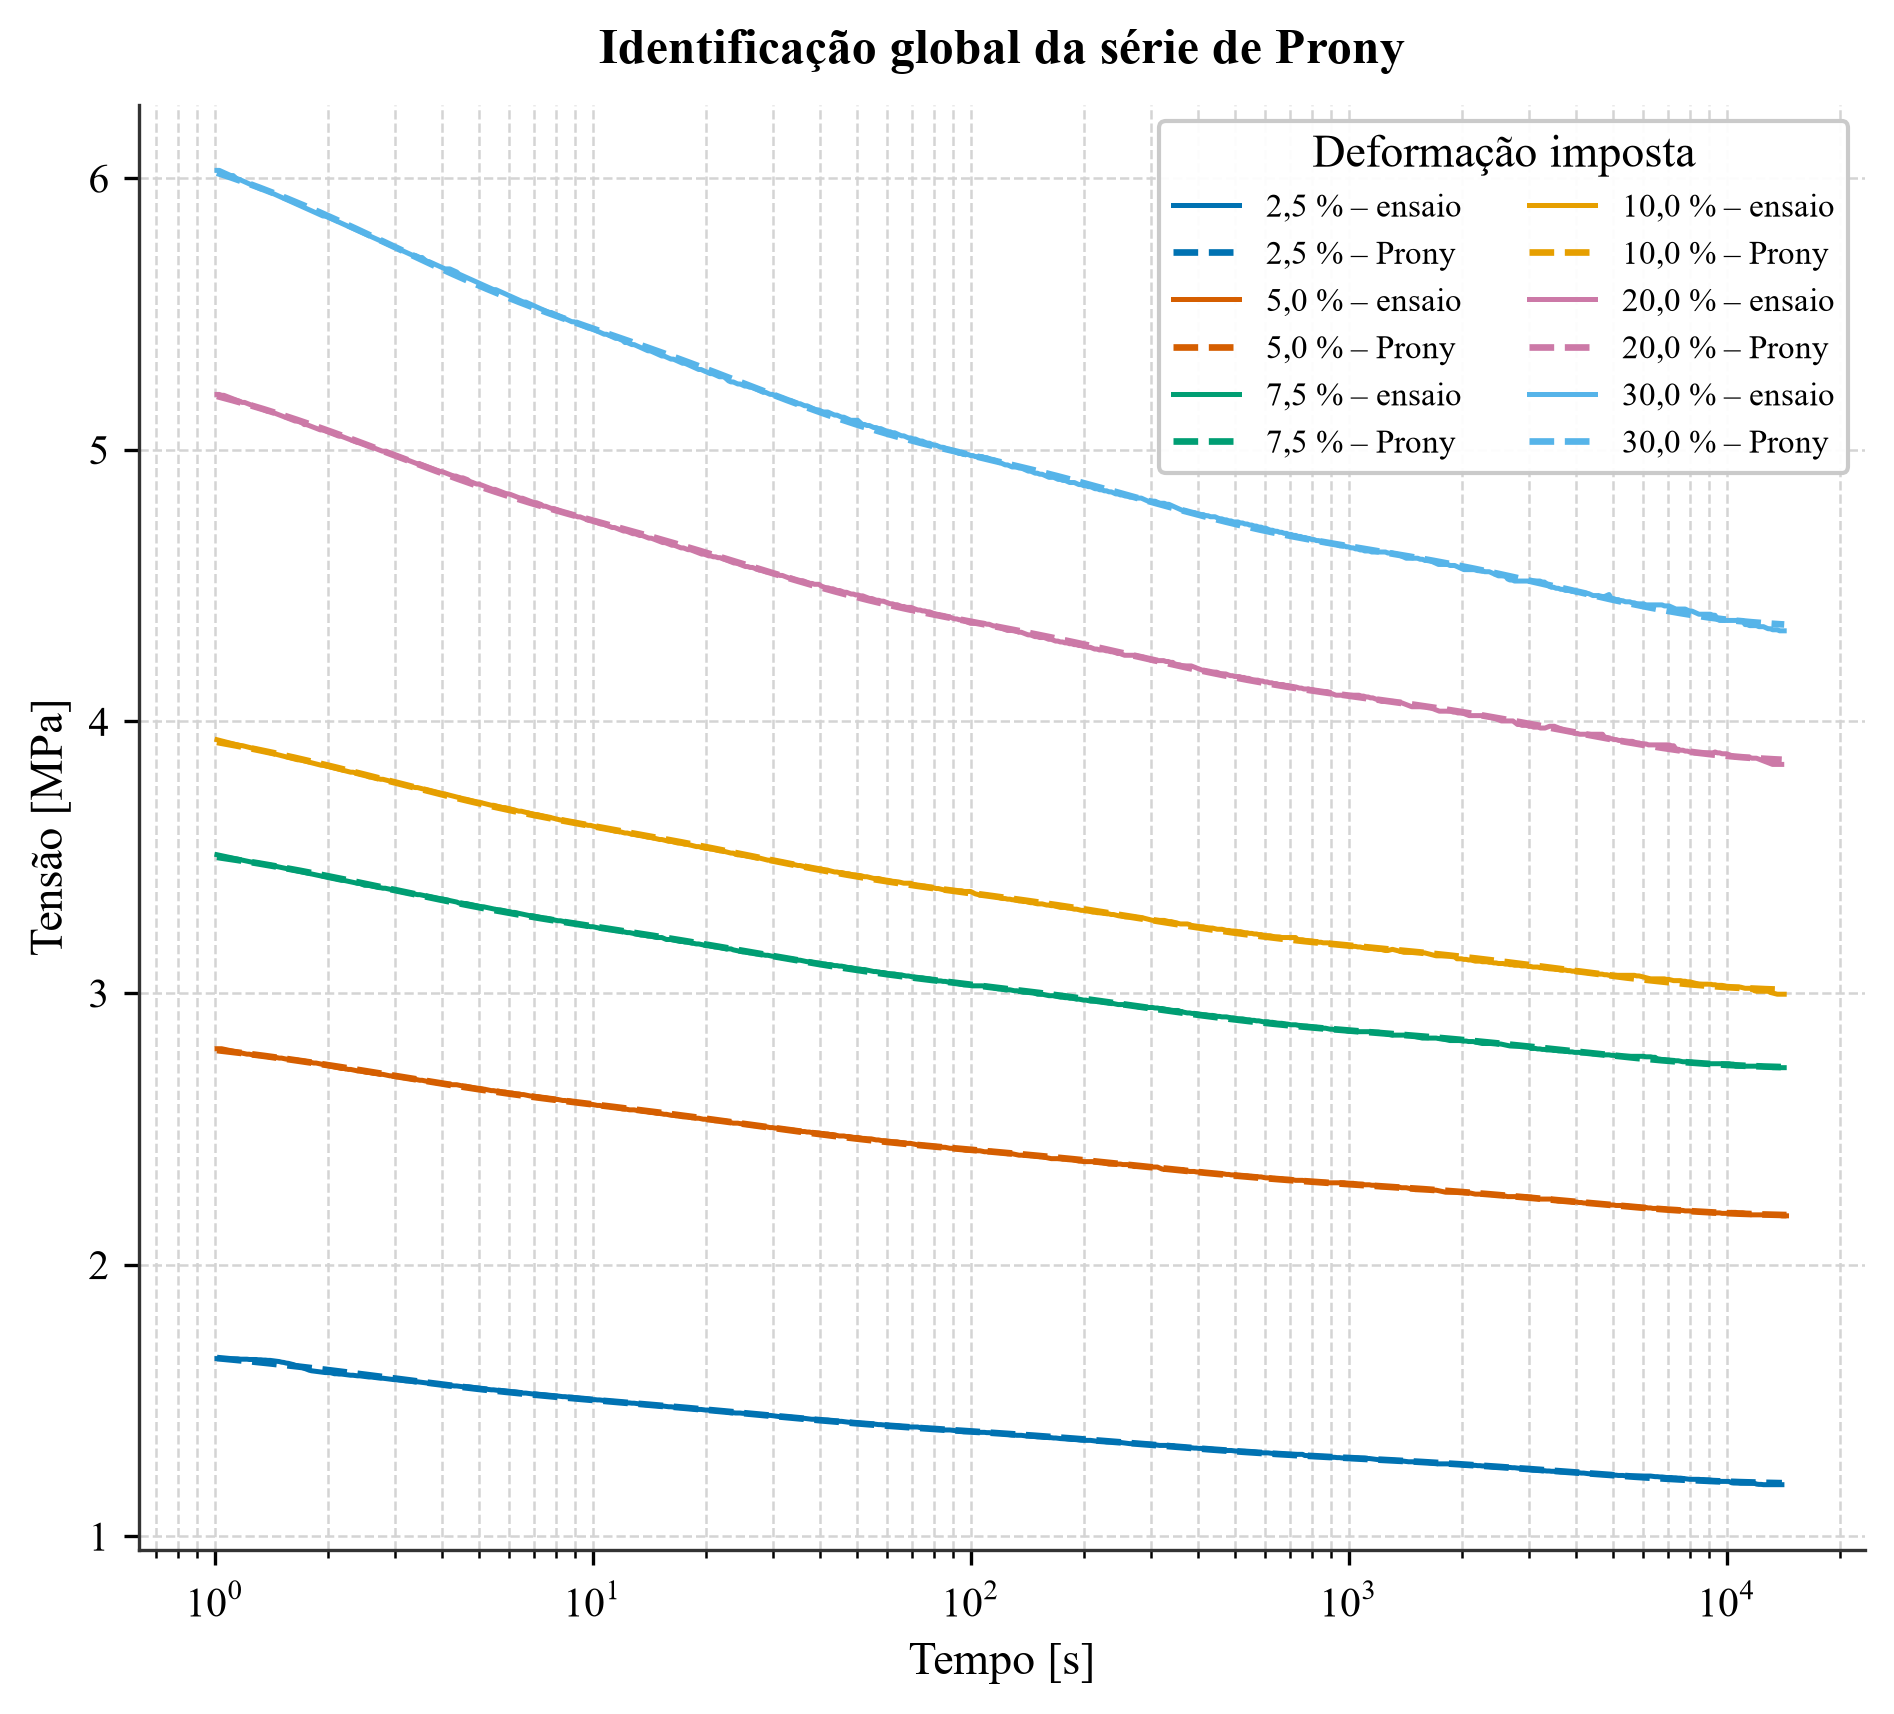
\includegraphics[width=0.88\textwidth]{pics/all-relaxation-fits.png}
  \caption{Ajustes da resposta de relaxação nos seis níveis de deformação.}
  \label{fig:ajustes-relaxacao}
  \fonte{Autoria própria.}
\end{figure}

A Tabela~\ref{tab:qualidade-ajustes-relaxacao} permite comparar os erros
entre os níveis de deformação. O RMSE varia de
$0{,}0022\,\mathrm{MPa}$ a $0{,}0074\,\mathrm{MPa}$, e o MAE, de
$0{,}0018\,\mathrm{MPa}$ a $0{,}0061\,\mathrm{MPa}$. Embora os erros
absolutos sejam maiores nas curvas de maior tensão, os valores de $R^2$
permanecem elevados em todos os níveis. A variação dos coeficientes
identificados entre as curvas também mostra por que uma única curva
linear não representa necessariamente toda a faixa de deformações:
para a representação PSM, os coeficientes das curvas individuais foram
regredidos em funções polinomiais de grau quatro.

\begin{table}[htb]
  \caption{Qualidade dos ajustes de relaxação por nível de deformação.}
  \label{tab:qualidade-ajustes-relaxacao}
  \centering
  \begin{tabular}{ccccc}
    \hline
    Deformação & $\sigma_0$ & RMSE & MAE & $R^2$\\
    $(\%)$ & $(\mathrm{MPa})$ & $(\mathrm{MPa})$
      & $(\mathrm{MPa})$ & $-$\\
    \hline
    2,5 & 1,1925 & 0,0032 & 0,0023 & 0,9994\\
    5,0 & 2,1794 & 0,0022 & 0,0018 & 0,9998\\
    7,5 & 2,7232 & 0,0031 & 0,0027 & 0,9998\\
    10,0 & 3,0071 & 0,0044 & 0,0036 & 0,9997\\
    20,0 & 3,8518 & 0,0055 & 0,0046 & 0,9998\\
    30,0 & 4,3486 & 0,0074 & 0,0061 & 0,9998\\
    \hline
  \end{tabular}
  \fonte{Autoria própria.}
\end{table}

Na comparação de validação, o modelo identificado com os próprios tempos
resultou em RMSE médio de $0{,}0280\,\mathrm{MPa}$ para todos os níveis,
enquanto o modelo publicado por \citeonline{Caire2011} apresentou RMSE
médio de $0{,}0637\,\mathrm{MPa}$ sobre o mesmo conjunto experimental.
O uso dos tempos de Caire combinado aos dados próprios forneceu RMSE médio
de $0{,}0316\,\mathrm{MPa}$, evidenciando que a identificação foi mais
consistente com os ensaios utilizados neste trabalho. A reprodução direta
das curvas de Prony tabuladas por Caire apresentou coerência geral em
regiões próximas à parte inicial da resposta, mas diferenças nas escalas
do decaimento mostram que os parâmetros publicados não são reproduzidos
exatamente pelas tabelas fornecidas na própria tese. Para a frequência
harmônica de $0{,}04\,\mathrm{Hz}$, o modelo próprio forneceu
$G'(0{,}2512)\cong78{,}82\,\mathrm{MPa}$ e
$G''(0{,}2512)\cong4{,}29\,\mathrm{MPa}$ no termo linear. A diferença
entre os RMSE médios indica melhor aderência dos parâmetros identificados
à base digitalizada empregada; não demonstra, por si só, superioridade
geral do modelo nem validação experimental independente, pois os dados
usados são os mesmos que fundamentaram a identificação.

\subsection{Reprodução da Resposta Estrutural}
\label{sec:reproducao-solucao-estrutural}

Antes da comparação entre geometrias, a resposta da configuração linear
foi verificada pela comparação das soluções obtidas com expansão até a
primeira, segunda e terceira ordens. As curvaturas máximas na raiz do
enrijecedor foram $0{,}3654$, $0{,}3768$ e
$0{,}3761\,\mathrm{m^{-1}}$, respectivamente. A diferença entre as
segunda e terceira ordens foi de aproximadamente $0{,}18\,\%$, mostrando
que a inclusão da terceira ordem alterou pouco a curvatura máxima em
relação à solução de segunda ordem. A proximidade desses dois resultados
indica baixa sensibilidade a essa parcela adicional, para a configuração
e as condições analisadas; não constitui uma estimativa do erro absoluto
da solução.

\begin{table}[htb]
  \caption{Sensibilidade da curvatura máxima à ordem da expansão perturbativa.}
  \label{tab:ordem-perturbativa}
  \centering
  \begin{tabular}{ccc}
    \hline
    Ordem & $\kappa_{\mathrm{raiz,max}}$ &
      $\kappa_{\mathrm{raiz,min}}$\\
    & $(\mathrm{m^{-1}})$ & $(\mathrm{m^{-1}})$\\
    \hline
    1 & 0,3654 & 0,1341\\
    2 & 0,3768 & 0,1454\\
    3 & 0,3761 & 0,1461\\
    \hline
  \end{tabular}
  \fonte{Autoria própria.}
\end{table}

Para a geometria de referência E1, o máximo absoluto de curvatura foi
$0{,}3761\,\mathrm{m^{-1}}$, localizado na extremidade superior do
enrijecedor, isto é, em $s=0\,\mathrm{m}$ no início da solução. Esse ponto
também correspondeu à maior deformação externa do poliuretano,
$13{,}16\,\%$. O raio mínimo associado foi $2{,}6586\,\mathrm{m}$, maior
que o MBR adotado de $2{,}00\,\mathrm{m}$. Como o limite de curvatura
correspondente ao MBR é $1/\mathrm{MBR}=0{,}50\,\mathrm{m^{-1}}$, a
curvatura máxima de E1 permanece abaixo desse limite. O resultado fornece
a referência estrutural para comparar as geometrias adaptadas, sem
implicar que as dimensões originalmente publicadas para outros casos
tenham sido reproduzidas sem alterações.

\begin{figure}[htb]
  \centering
  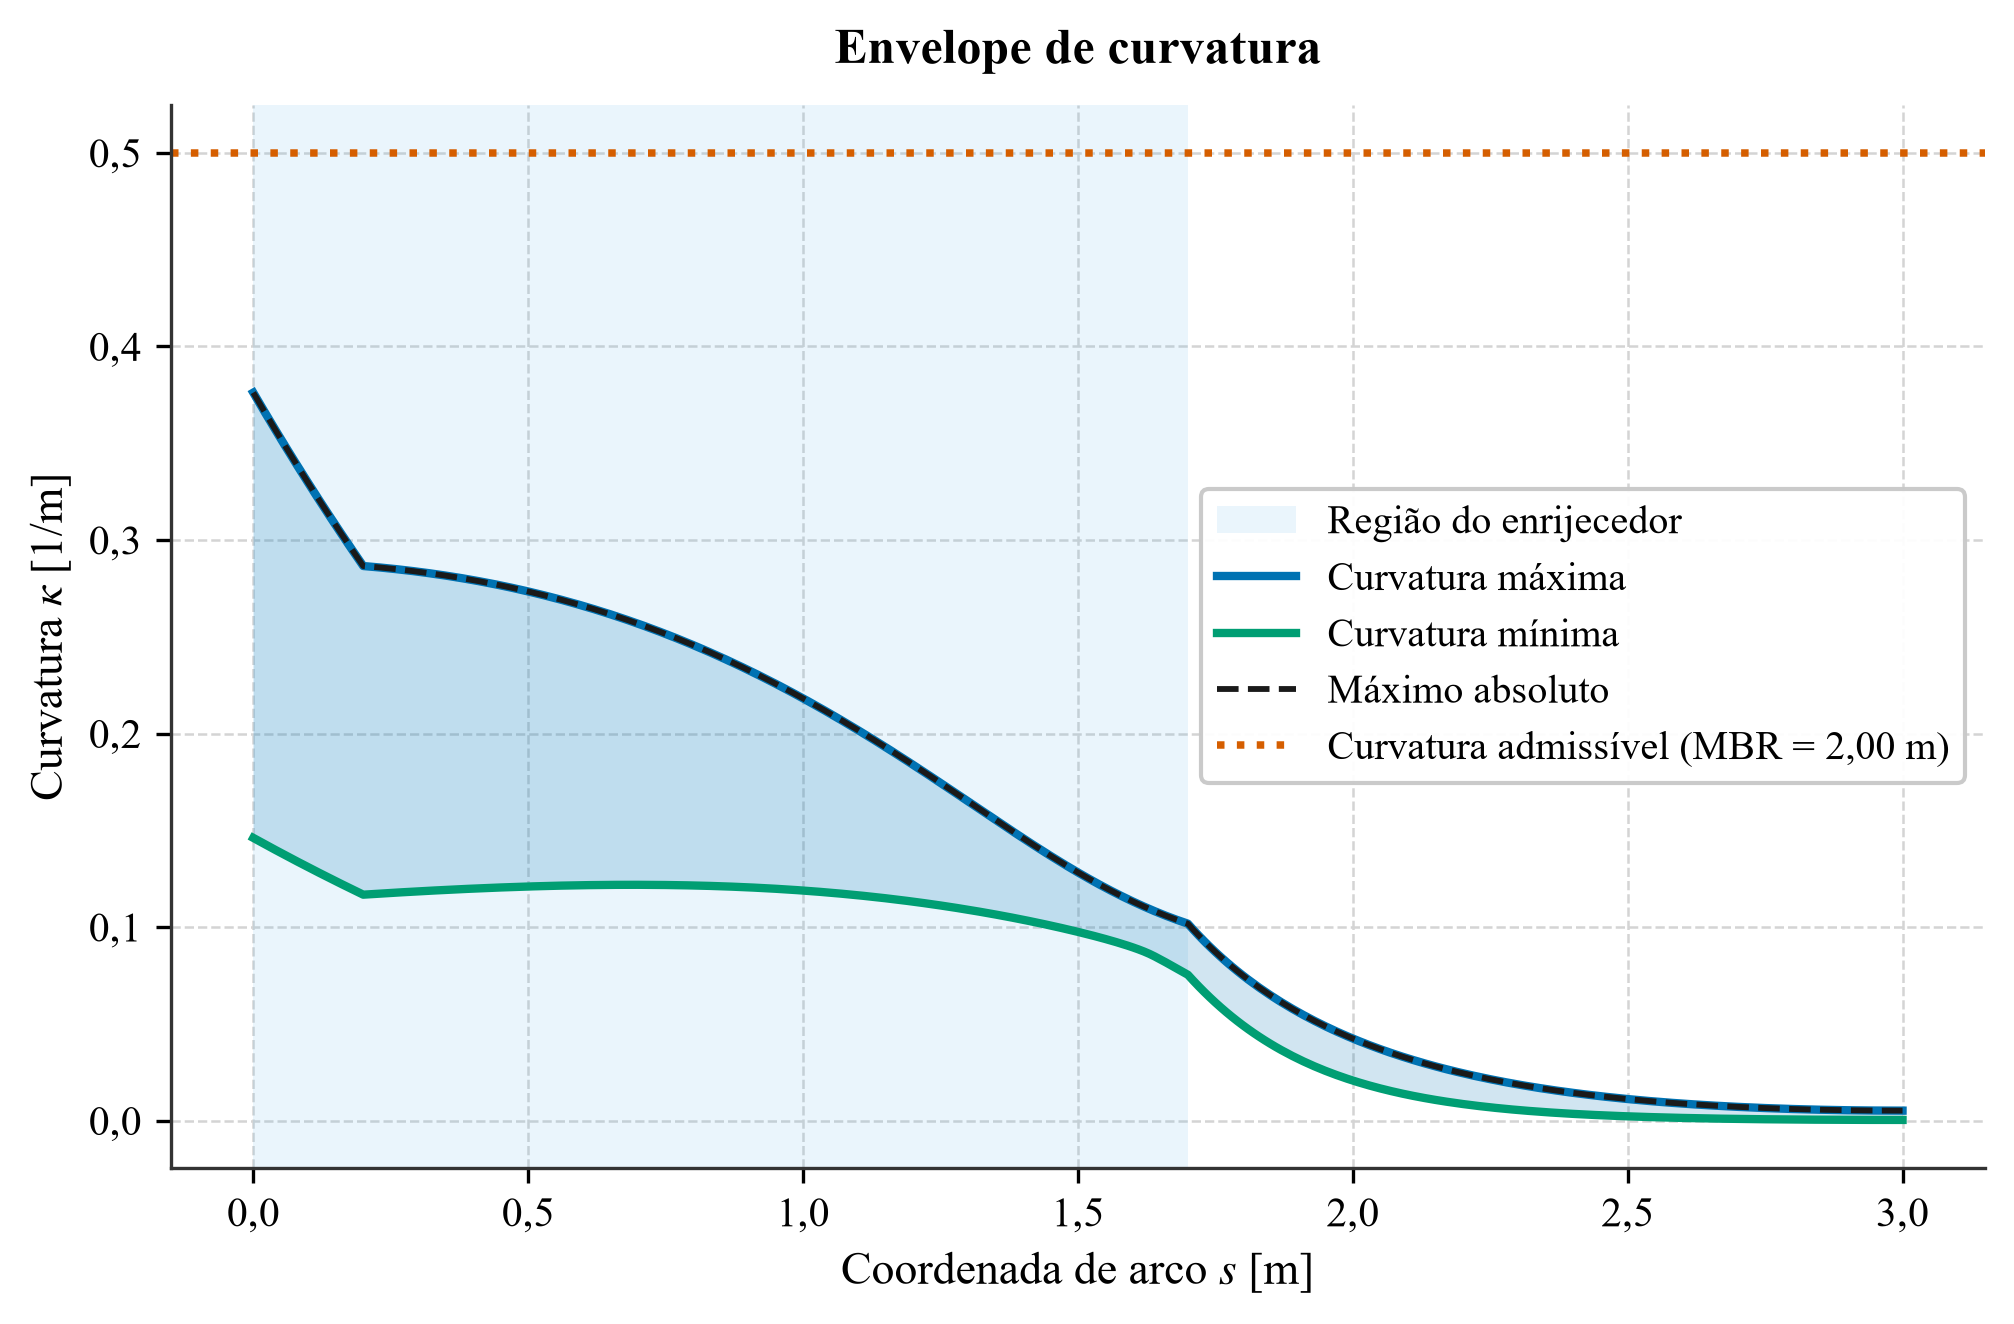
\includegraphics[width=0.86\textwidth]{pics/caire-curvature-envelope.png}
  \caption{Envelope de curvatura ao longo do comprimento da geometria E1.}
  \label{fig:envelope-curvatura-e1}
  \fonte{Autoria própria.}
\end{figure}

\section{Solução do Estudo de Caso}
\label{sec:solucao-do-estudo-de-caso}

Com a resposta de referência examinada, o procedimento é aplicado às três
geometrias do estudo de caso, mantendo-se as condições de carregamento,
material e linha flexível. Além de verificar os limites de deformação do
poliuretano e de raio mínimo, comparam-se as margens obtidas e o volume de
cada enrijecedor.

\subsection{Resultados Obtidos}
\label{sec:resultados-obtidos}

Para comparar os casos em uma mesma base, os resultados foram calculados
com carregamento, frequência e modelo constitutivo comuns, reconstruindo
361 fases por ciclo. Os máximos da
Tabela~\ref{tab:resultados-dimensionamento} são estimativas nos pontos da
malha espacial e temporal; por isso, suas magnitudes e posições dependem
das resoluções adotadas e da aproximação perturbativa.

\begin{table}[htb]
  \caption{Síntese dos resultados do dimensionamento das três geometrias.}
  \label{tab:resultados-dimensionamento}
  \centering
  \begin{tabular}{cccccccc}
    \hline
    Caso & $D_b$ & $L_e$ & Volume &
      $\kappa_{\mathrm{max}}$ & $\varepsilon_{\mathrm{max}}$ &
      $\mathrm{FS}_{global}$ & Situação\\
    & $(\mathrm{m})$ & $(\mathrm{m})$ & $(\mathrm{m^3})$
      & $(\mathrm{m^{-1}})$ & $(\%)$ & $-$ & $-$\\
    \hline
    E1 & 0,700 & 1,700 & 0,2539 & 0,3761 & 13,16 & 1,139 & Aprovado\\
    E2 & 0,660 & 1,900 & 0,2411 & 0,4426 & 14,61 & 1,027 & Aprovado\\
    E3 & 0,575 & 2,350 & 0,2204 & 0,6364 & 18,30 & 0,786 & Reprovado\\
    \hline
  \end{tabular}
  \fonte{Autoria própria.}
\end{table}

Na geometria E1, o fator global foi governado pela deformação do
poliuretano: $\mathrm{FS}_{\varepsilon}=1{,}1394$, enquanto
$\mathrm{FS}_{\mathrm{MBR}}=1{,}3293$. A deformação máxima ficou
$1{,}84$ ponto percentual abaixo do limite de $15\,\%$, e o raio mínimo
de $2{,}6586\,\mathrm{m}$ superou o MBR em $0{,}6586\,\mathrm{m}$.
Assim, os dois critérios foram atendidos, com maior proximidade do limite
de deformação.

Em E2, a deformação máxima de $14{,}61\,\%$ ficou apenas
$0{,}39$ ponto percentual abaixo do limite, resultando em
$\mathrm{FS}_{\mathrm{global}}=1{,}0269$. Esse valor indica atendimento
ao critério no caso calculado, mas uma margem menor que a de E1. O raio
mínimo de $2{,}2592\,\mathrm{m}$ também permaneceu acima do MBR de
$2{,}00\,\mathrm{m}$; portanto, como em E1, foi a deformação que
governou a avaliação.

A geometria E3 apresentou deformação máxima de $18{,}30\,\%$, superior ao
limite adotado, e raio mínimo de $1{,}5714\,\mathrm{m}$, inferior ao
MBR. Esse raio corresponde a uma curvatura de aproximadamente
$0{,}6364\,\mathrm{m^{-1}}$, acima do limite de
$0{,}50\,\mathrm{m^{-1}}$. Os fatores associados à deformação e ao MBR
foram, respectivamente, $0{,}8198$ e $0{,}7857$; o segundo foi o menor
e, portanto, governou a reprovação. Logo, E3 não atende a nenhum dos dois
critérios, apesar de apresentar o menor volume e o maior comprimento
entre as configurações avaliadas.

\subsection{Comparação dos Resultados}
\label{sec:comparacao-resultados}

O aumento do comprimento total não produziu uma redução proporcional da
curvatura crítica nas geometrias avaliadas. E1, com volume de
$0{,}2539\,\mathrm{m^3}$, apresentou curvatura de
$0{,}3761\,\mathrm{m^{-1}}$. E2 apresentou volume ligeiramente menor,
$0{,}2411\,\mathrm{m^3}$, porém curvatura maior,
$0{,}4426\,\mathrm{m^{-1}}$. E3 apresentou o menor volume,
$0{,}2204\,\mathrm{m^3}$, mas a maior curvatura,
$0{,}6364\,\mathrm{m^{-1}}$. Os resultados indicam que o diâmetro da base
e a distribuição longitudinal da rigidez têm influência mais direta sobre
a resposta do que o volume isoladamente. Essa interpretação deve ser
considerada em conjunto com o fato de que as geometrias também diferem
nos comprimentos cilíndrico e cônico e no comprimento de linha após o
enrijecedor; assim, os resultados não isolam o efeito de uma única
dimensão.

\begin{figure}[htb]
  \centering
  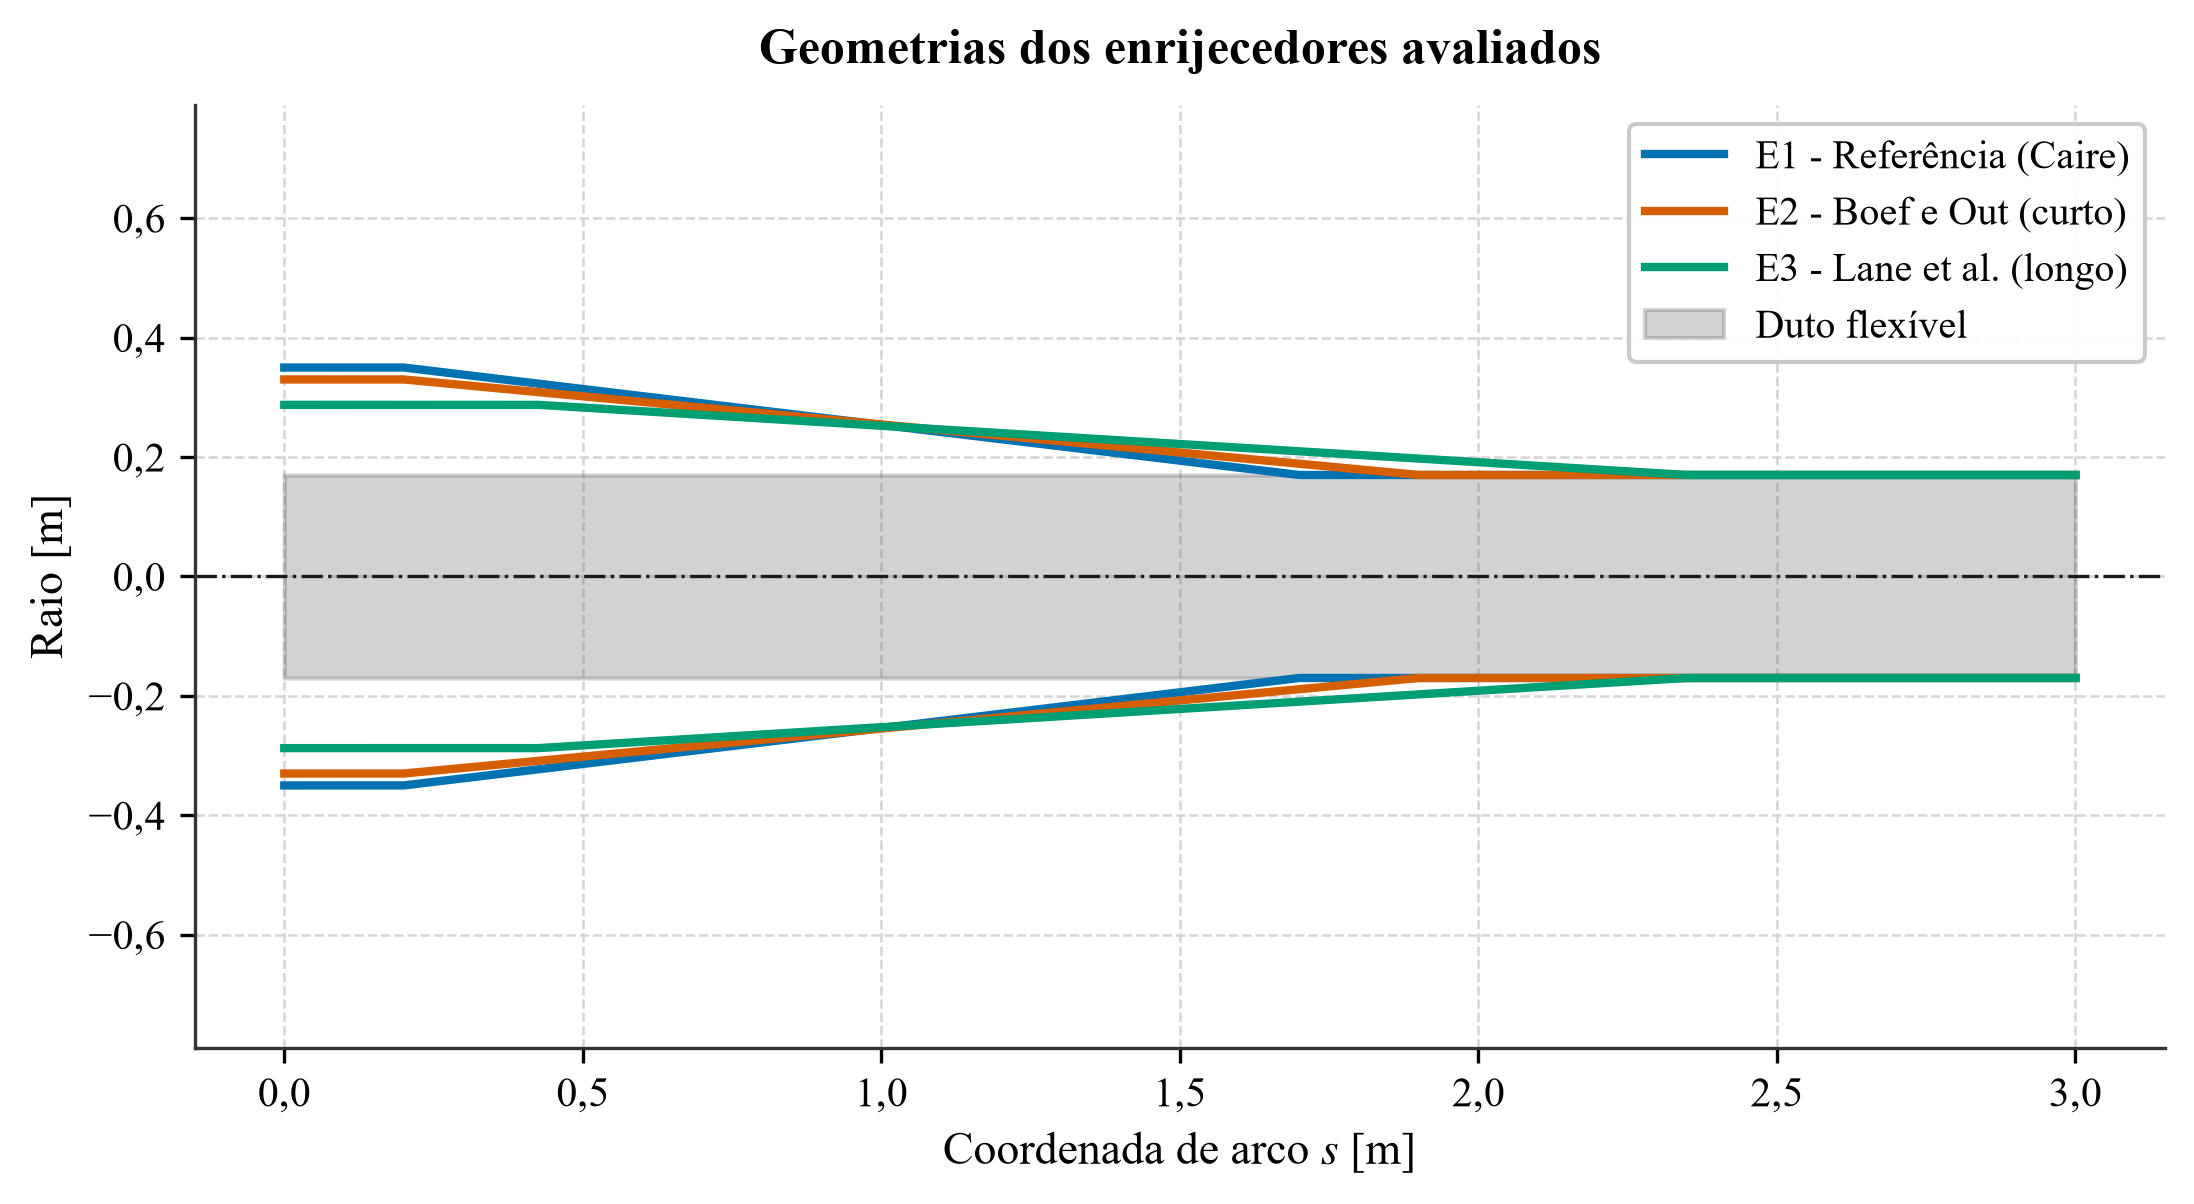
\includegraphics[width=0.86\textwidth]{pics/comparacao-geometria.png}
  \caption{Comparação das geometrias dos enrijecedores E1, E2 e E3.}
  \label{fig:comparacao-geometria}
  \fonte{Autoria própria.}
\end{figure}

\begin{figure}[htb]
  \centering
  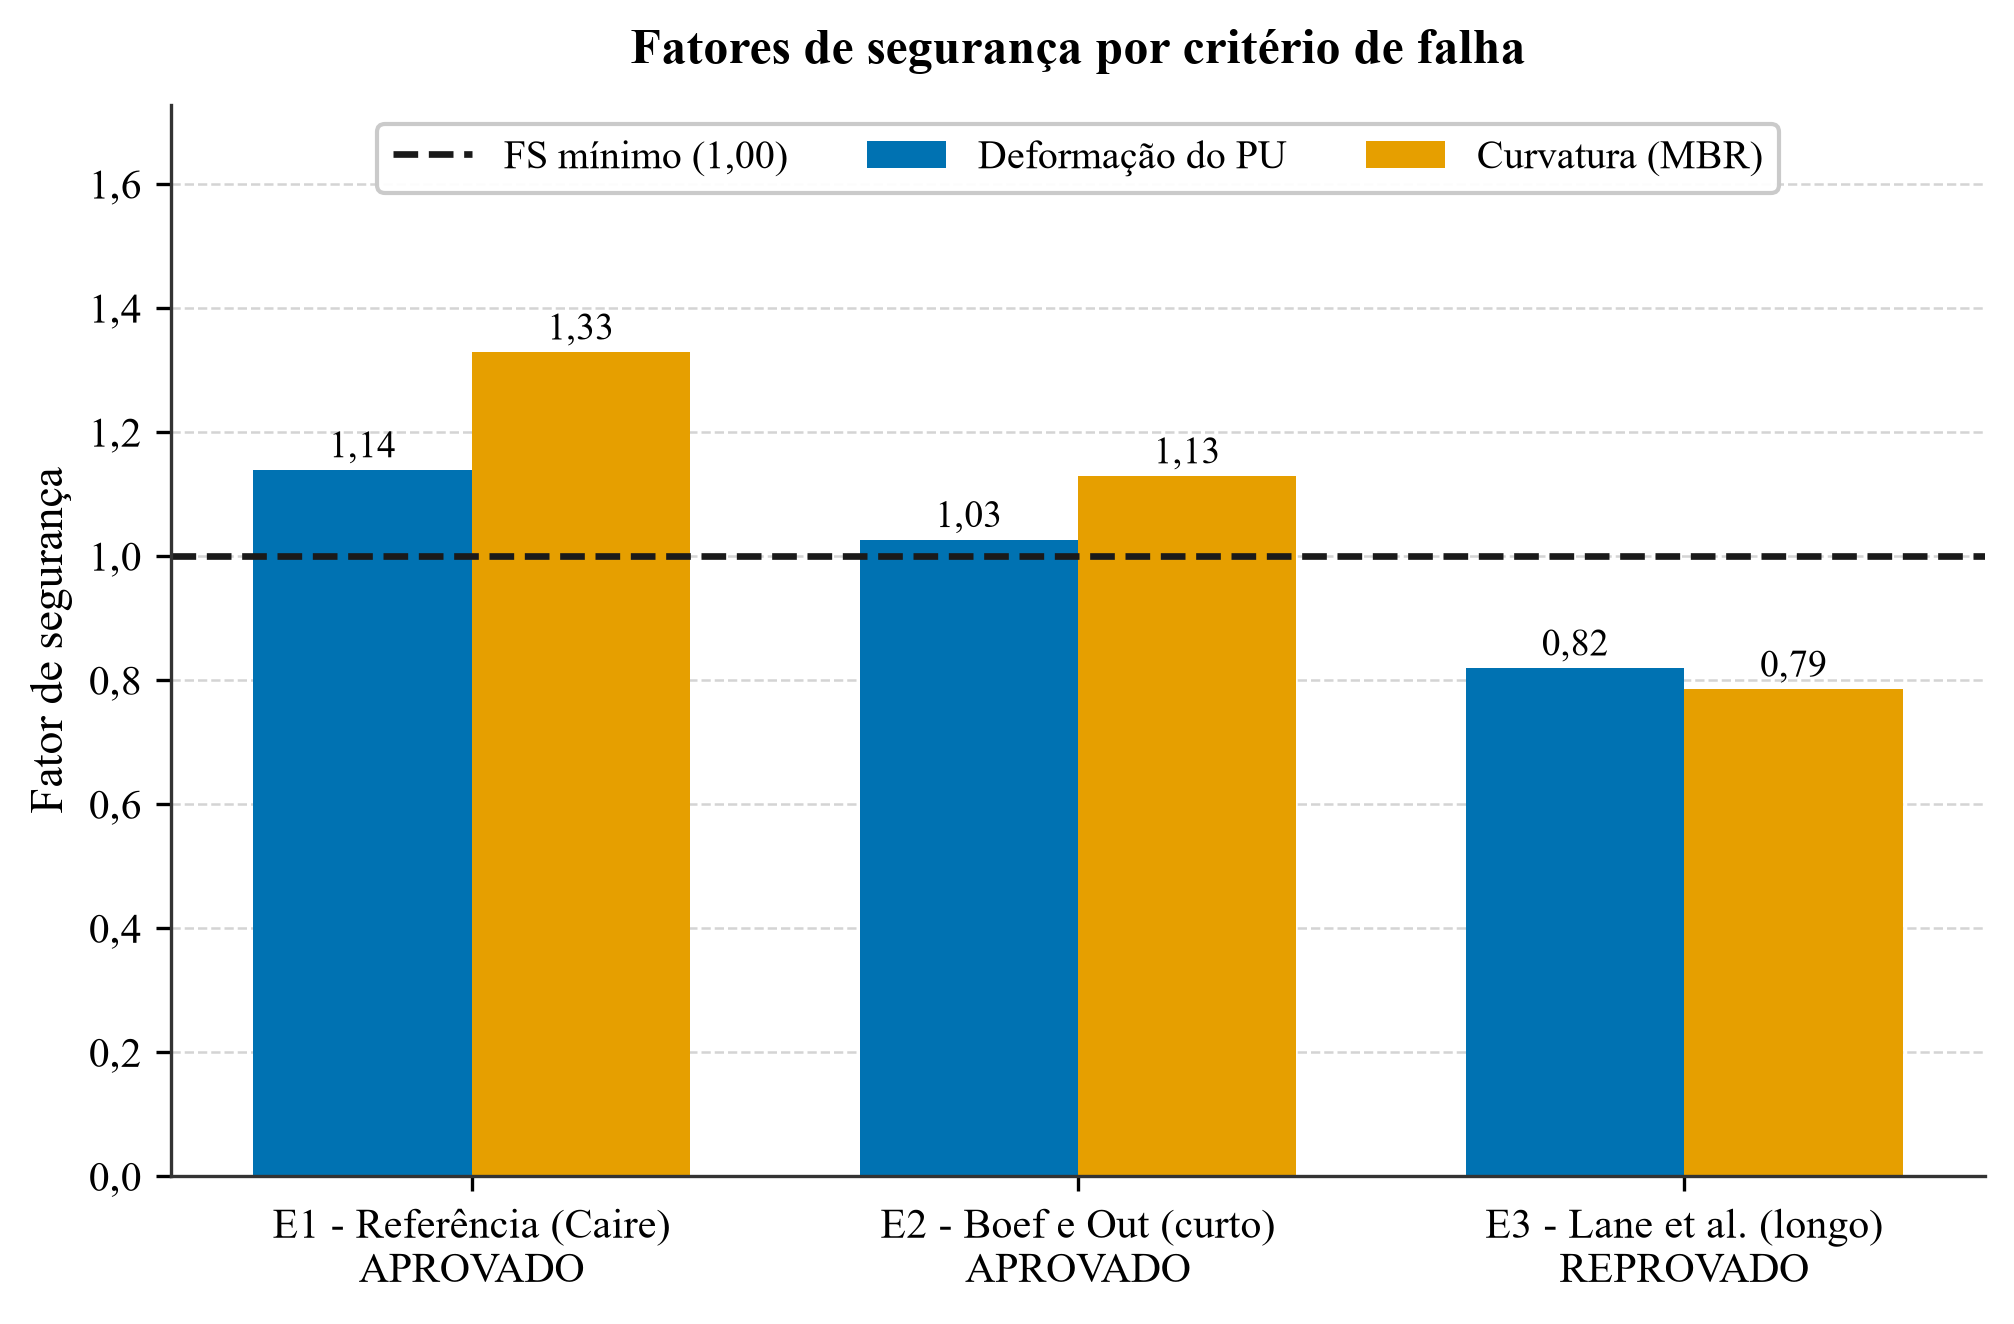
\includegraphics[width=0.86\textwidth]{pics/fatores-seguranca.png}
  \caption{Fatores de segurança por critério e fator global das geometrias E1, E2 e E3.}
  \label{fig:fatores-seguranca}
  \fonte{Autoria própria.}
\end{figure}

Entre as geometrias aprovadas, E1 apresentou maior margem global
($1{,}1394$), em oposição à E2 ($1{,}0269$). E1 também apresentou menor
curvatura absoluta e menor deformação máxima que E2. Todavia, E2 possui
volume aproximadamente $5\,\%$ menor, valor obtido pela relação
$0{,}2411/0{,}2539-1$. Portanto, a escolha entre E1 e E2 dependeria da
priorização da margem em relação aos critérios adotados ou da economia
de material. A diferença de volume, por si só, não permite concluir que
E2 seja uma solução mais eficiente, pois sua margem de deformação é
reduzida e os dois casos não foram objeto de otimização.

Por fim, os resultados não constituem uma otimização global das dimensões.
A aproximação é válida dentro da expansão perturbativa adotada, da
frequência analisada, das propriedades viscoelásticas identificadas e do
domínio finito empregado. A sensibilidade ao comprimento do domínio e a
incorporação de efeitos não lineares e térmicos permanecem como etapas
necessárias para uma extrapolação do modelo a condições reais de projeto.

% ----------------------------------------------------------------------

\chapter{Conclusão}
\label{sec:conclusao}

\section{Trabalhos Futuros}
\label{sec:trabalhos-futuros}

%%% ====================================================================
%%% Início da parte pós-textual do documento.

\postextual


%%% Referências Bibliográfica
\bibliography{referencias}

%%% Início dos apêndices ---------------------------------------------

\apendices

%%% A linha abaixo impede que as seções, subseções, etc. dos apêndices e anexos
%%% sejam mostradas no Sumário.
\addtocontents{toc}{\protect\setcounter{tocdepth}{0}}

\partapendices*

% --------------------------------------------------------------------

\chapter{Demonstração do Teorema Loren Ipsum}

% --------------------------------------------------------------------
%%% Início dos anexos ------------------------------------------------
\anexos

\partanexos*

\chapter{Exemplo de lombada}

\hspace*{0mm}\fbox{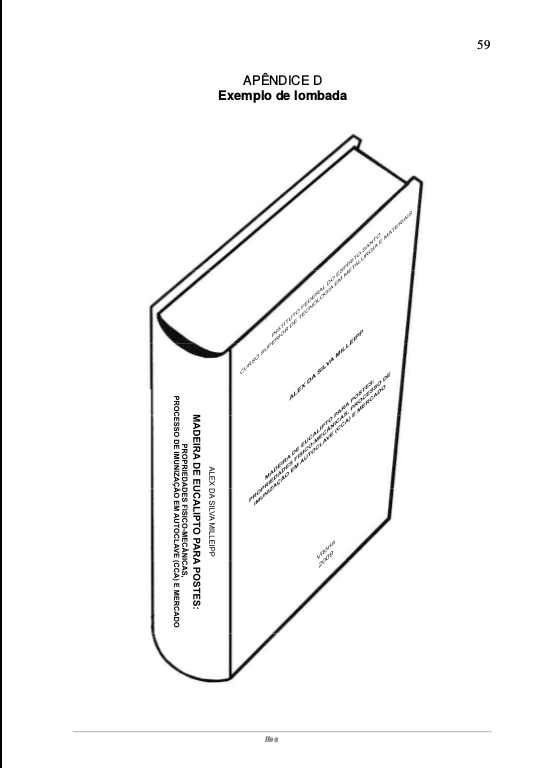
\includegraphics[scale=0.8]{pics/normas-ifes-apendice-d.png}}

\end{document}